\documentclass[aps,prb,superscriptaddress,floatfix,onecolumn]{revtex4}
\usepackage[raggedright]{titlesec} 
\usepackage{times}
\usepackage{graphicx}% Include figure files
\usepackage{amsmath}
\usepackage{amssymb}
\usepackage{subfigure}
\usepackage{color}
\usepackage{ulem}
\usepackage{sidecap}
\usepackage{floatrow}
\usepackage{hyperref}
%\usepackage[utf8]{inputenc}
\usepackage{listings}
\usepackage{makecell}

\newcommand{\red}[1]{\textcolor{red}{#1}}
\newcommand{\blue}[1]{\textcolor{blue}{#1}}

\newcommand{\mH}{\mathcal{H}}
\newcommand{\mT}{\mathcal{T}}
\newcommand{\mV}{\mathcal{V}}
\newcommand{\mP}{\mathcal{P}}
\newcommand{\mS}{\mathcal{S}}

\definecolor{codegreen}{rgb}{0,0.6,0}
\definecolor{codegray}{rgb}{0.5,0.5,0.5}
\definecolor{codepurple}{rgb}{0.58,0,0.82}
\definecolor{backcolour}{rgb}{0.95,0.95,0.92}
 
\lstdefinestyle{mystyle}{
    backgroundcolor=\color{backcolour},   
    commentstyle=\color{codegreen},
    keywordstyle=\color{magenta},
    numberstyle=\tiny\color{codegray},
    stringstyle=\color{codepurple},
    basicstyle=\footnotesize,
    breakatwhitespace=false,         
    breaklines=true,                 
    captionpos=b,                    
    keepspaces=true,                 
    numbers=left,                    
    numbersep=5pt,                  
    showspaces=false,                
    showstringspaces=false,
    showtabs=false,                  
    tabsize=2
}
 
\lstset{style=mystyle}


\begin{document}

\title{TBM$^3$ : Tight Binding Model for Materials at Mesoscale}

\author{Yuan-Yen Tai}
\affiliation{Theoretical Division, Los Alamos National Laboratory, Los Alamos, New Mexico 87545, USA}
\author{Wei Zhu}
\affiliation{Theoretical Division, Los Alamos National Laboratory, Los Alamos, New Mexico 87545, USA}
\affiliation{Center for Nonlinear Studies, Los Alamos National Laboratory, Los Alamos, New Mexico 87545, USA}
\author{Hongchul Choi}
\affiliation{Theoretical Division, Los Alamos National Laboratory, Los Alamos, New Mexico 87545, USA}

\author{Jian-Xin Zhu}
\affiliation{Theoretical Division, Los Alamos National Laboratory, Los Alamos, New Mexico 87545, USA}
\affiliation{Center for Integrated Nanotechnologies, Los Alamos National Laboratory, Los Alamos, New Mexico 87545, USA}

\date{\today}

\begin{abstract}
%TBM$^3$ is an open source package for computational simulations of quantum materials at multiscale in length and time. 
%The project is originated to investigate the multiferroic behavior in transition-metal-oxide heterostructure. 
%The framework has also been designed to study emergent phemona in other quantum materials like 2-dimensional transition-metal dichalcogenides, graphene, topological insulators, and skyrmion in materials, etc. 
%In the long term, we will enable the package for transport and time-resolved phenomena. 
%TBM$^3$ is currently a C++ based numerical tool package and framework for the design and construction of any kind of lattice structures with multi-orbital and spin degrees of freedom. 
%The fortran based portion of the package will be added in the near future. 
%The design of TBM$^3$ is in a highly flexible and reusable framework and the tight-binding parameters can be modeled or informed by DFT calculations. 
%It is currently GPU enabled and feature of CPU enabled MPI will be added in the future.
We present a new open-source package, called \textit{TBM$^3$}, for computational simulations of quantum materials at multiscale in length and time.
The project is well-suited to study the multiferroic behavior in transition-metal-oxide heterostructure,
electronic structure of quantum materials such as two-dimensional 
transition-metal dichalcogenides, graphene, topological insulators, and skyrmion in materials, to name a few.
TBM$^3$ is highly flexible for the design and construction of any kind of lattice structures with multi-orbital and spin degrees of freedom,
and user-friendly interface allows the tight-binding parameters loaded from density-functional-based calculations.
TBM$^3$ is currently a C++ based and GPU enabled, which makes it amenable to a high-level customisation. 
As a far-seeing plan, we will enable the TBM$^3$ package for quantum transport and time-resolved phenomena,
and feature of CPU enabled MPI will be added in the future.
\end{abstract}


\maketitle

\text{}\\\\\\

\begin{center}
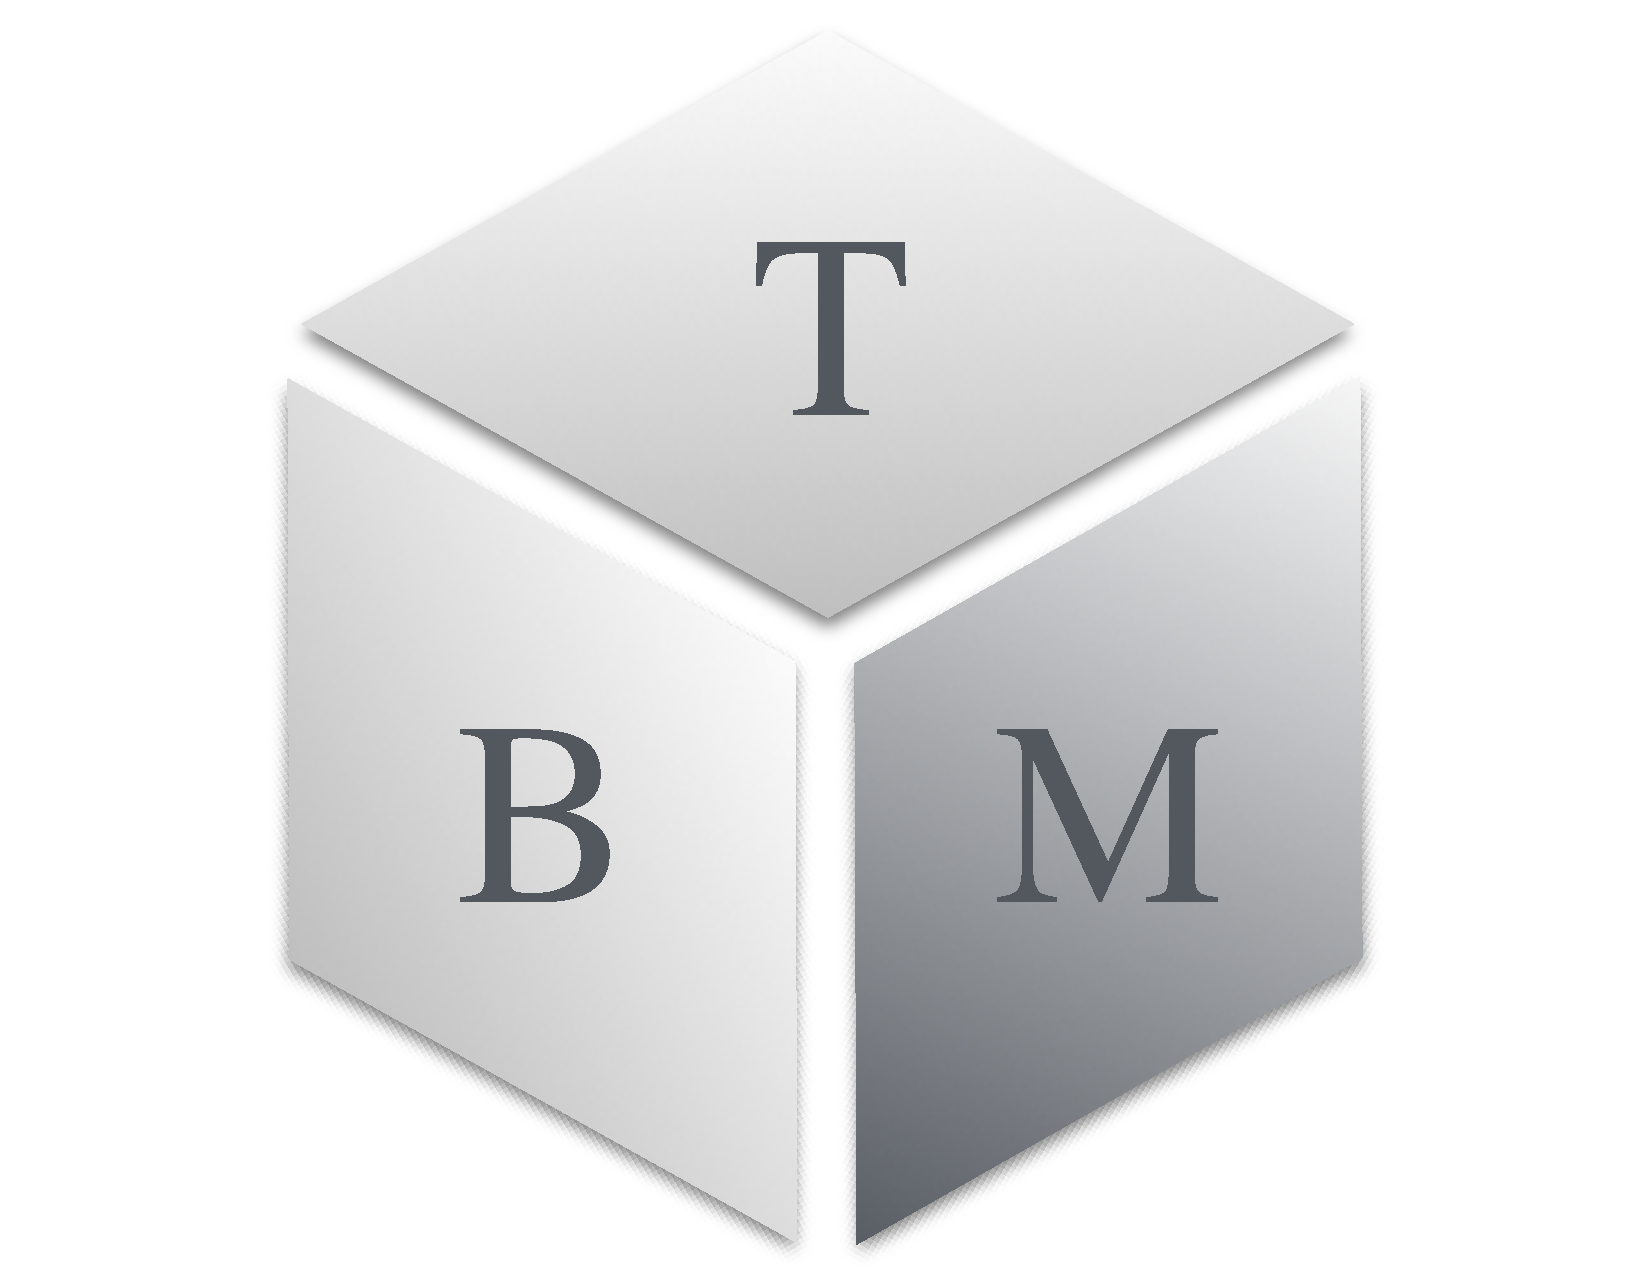
\includegraphics[scale=0.35]{TBMCube-LOGO.pdf}
\end{center}

%\clearpage
\clearpage
\tableofcontents
\begin{figure}
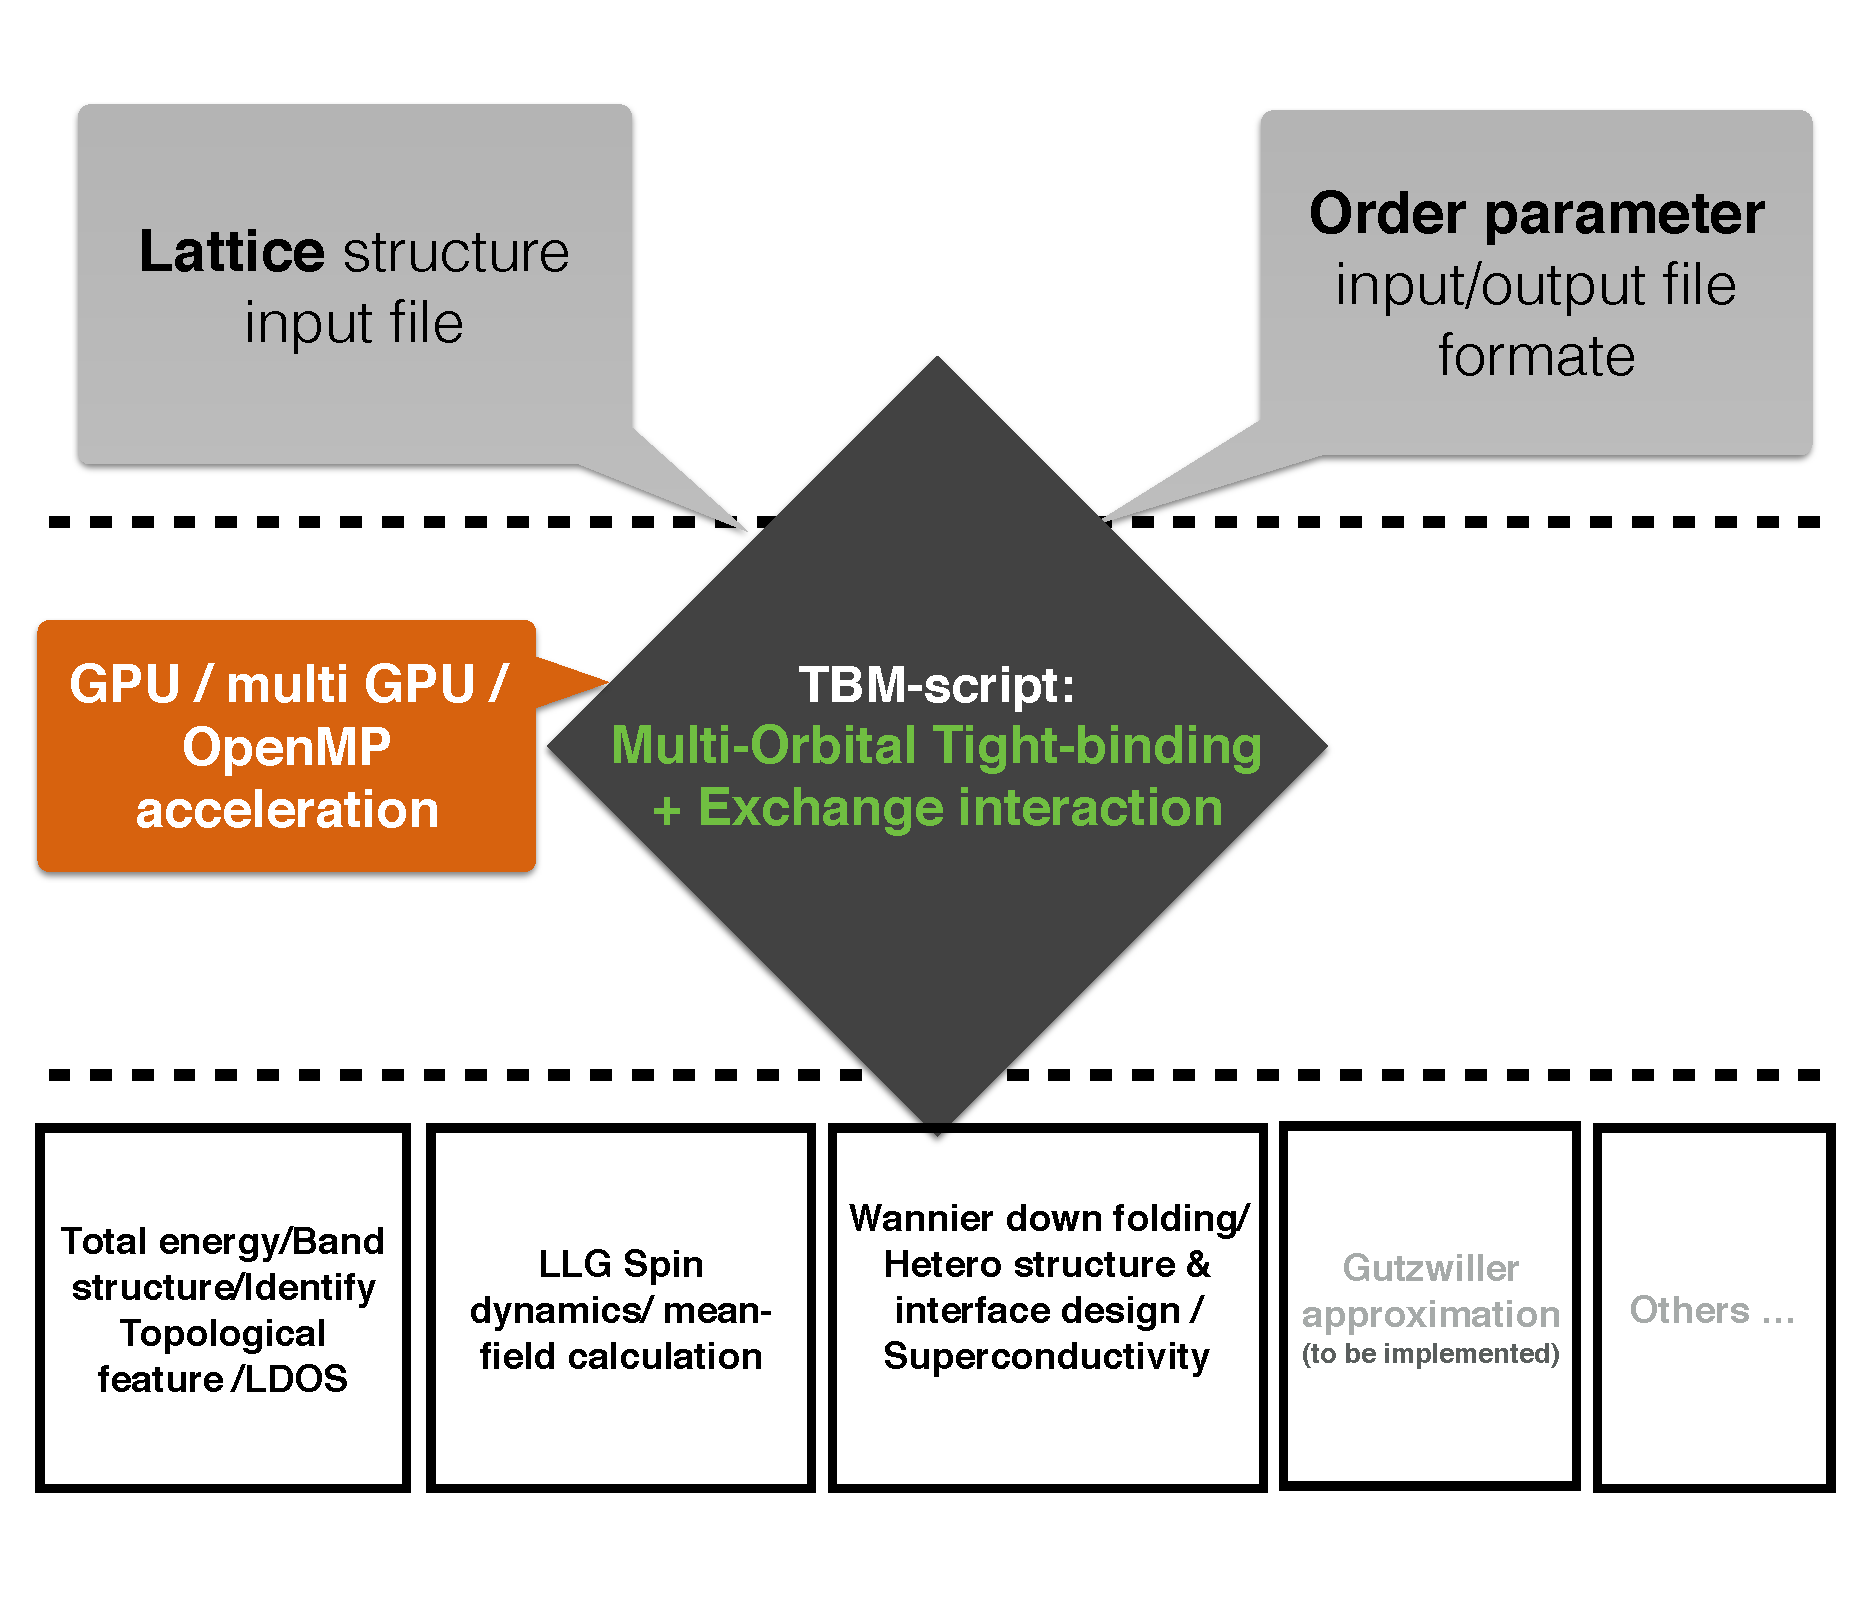
\includegraphics[scale=0.30]{./TBMCube.pdf}
\caption{The layout of TBM$^3$ structure.}
\label{TBMCube}
\end{figure}
\clearpage


\section{Introduction}
%There are many difficulties and challenges in study material properties in condensed matter theory. Overall, the problems can be subject into two categories:
Condensed matter physics is a branch of physics that deals with the physical properties of condensed phases of matter \cite{Philip_book}, 
with the help of physical laws of quantum mechanics and statistical mechanics. Overall, condensed matter physicists seek to:
\begin{enumerate}
\item 	Understand the basic physics phenomenon and discover new physics features in qualitative way;
\item 	Identify various material properties quantitatively and design functional materials with potential applications in the real world.
\end{enumerate}
To target problem \#1 and \#2, condensed matter theory physicists have created various theoretical and numerical tools, and explored a great amount of scientific applications for the modern technologies \cite{Cohen2008,Kohn1999}.

In the early days, physicists focused on the problem \#1. The normal strategy is to extract simplified and effective models from realistic systems,
by ignoring some complicate situations. The great advantage is that, it usually gives a clear picture of physical phenomena\cite{Baxter1999}, 
with examples including the Bogoliubov–de Gennes (BdG) equation for the study of superconductivity \cite{BdG,BCS}, the Heisenberg model for the study of magnetism \cite{Lenz,Ising,Bethe,Heisenberg}, the Hubbard model for the study of transition between conducting and insulating phases \cite{Hubbard}, the Haldane model for the study of topological properties, and so on so forth.
However, physicists also realize that it was not enough to identify material properties with only  effective models,
because lots of physical properties are material specific and sensitive to the environment such as temperature, pressure, doping, impurity and orbital details.
This is the shortcoming of effective models since lots of details were dropped in the beginning, 
which immediately inspires the problem \#2 : How can we capture material properties quantitatively?

Fortunately, inventing the density functional theory (DFT) for the study of physics and chemistry properties shed lights on the the problem \#2.
%In 1998, the Nobel Laureates Walter Kohn and John A. Pople decently approached by
%In the physics community, DFT is now developed into several computational tool packages 
Over the past years, there have appeared open source, freely accessible numerical packages
and libraries which contribute to widespread the use of DFT among the condensed matter community,
such as VASP \cite{vasp}, Wien2K \cite{win} and Quantum Espresso \cite{espresso}.
These tool packages are also called as the ``first principal calculations'', 
since they can capture many physical properties without (or with few) control parameters.
However, the DFT calculations are restricted by several limitations.
The first limitation is due to that the Coulomb interaction was treated in a Hatree-Fock scheme, therefore, 
DFT fails to capture the correlation effects correctly when the Coulomb interaction dominates over kinetic terms.
The second limitation is that the DFT Kohn-Sham equation requires very large computational resources even for a small size of system.
Therefore, it is too expensive to get full electronic structure even for  a large molecule or complex crystal structure.
Recently, the second limitation becomes more and more serious due to the demanding studies for 
impurity effect, interface physics and large size spin structure in multi dimensions \cite{Jones}.

To overcome the aforementioned limitations, people try to find a way to combine the advantages of 
the model formalism and the DFT calculations. In the ideal case, one can perform the DFT calculations on relatively small clusters, 
and then perform large-scale calculation based on the tight-bind model using DFT parameters as input. 
Supposed that Coulomb interactions could be suitably treated, this scheme is expected to provide an avenue to material science.
Here, we report a newly developed optimised open-source package, TBM$^3$,
which is indeed such kind of solution.
%is targeting to serve above problems (1 and 2) and trying to combine the efficiency of the model formalism and the accuracy of the DFT calculated parameters, see %Fig.~\ref{TBMCube}.
%On one hand, in using TBM$^3$, we can easily construct almost any kind of model in any kind of lattice structure just in several steps.
%On the other other, we can also apply the package to solve much larger lattice size with the DFT guided input parameters.

%\begin{figure}
%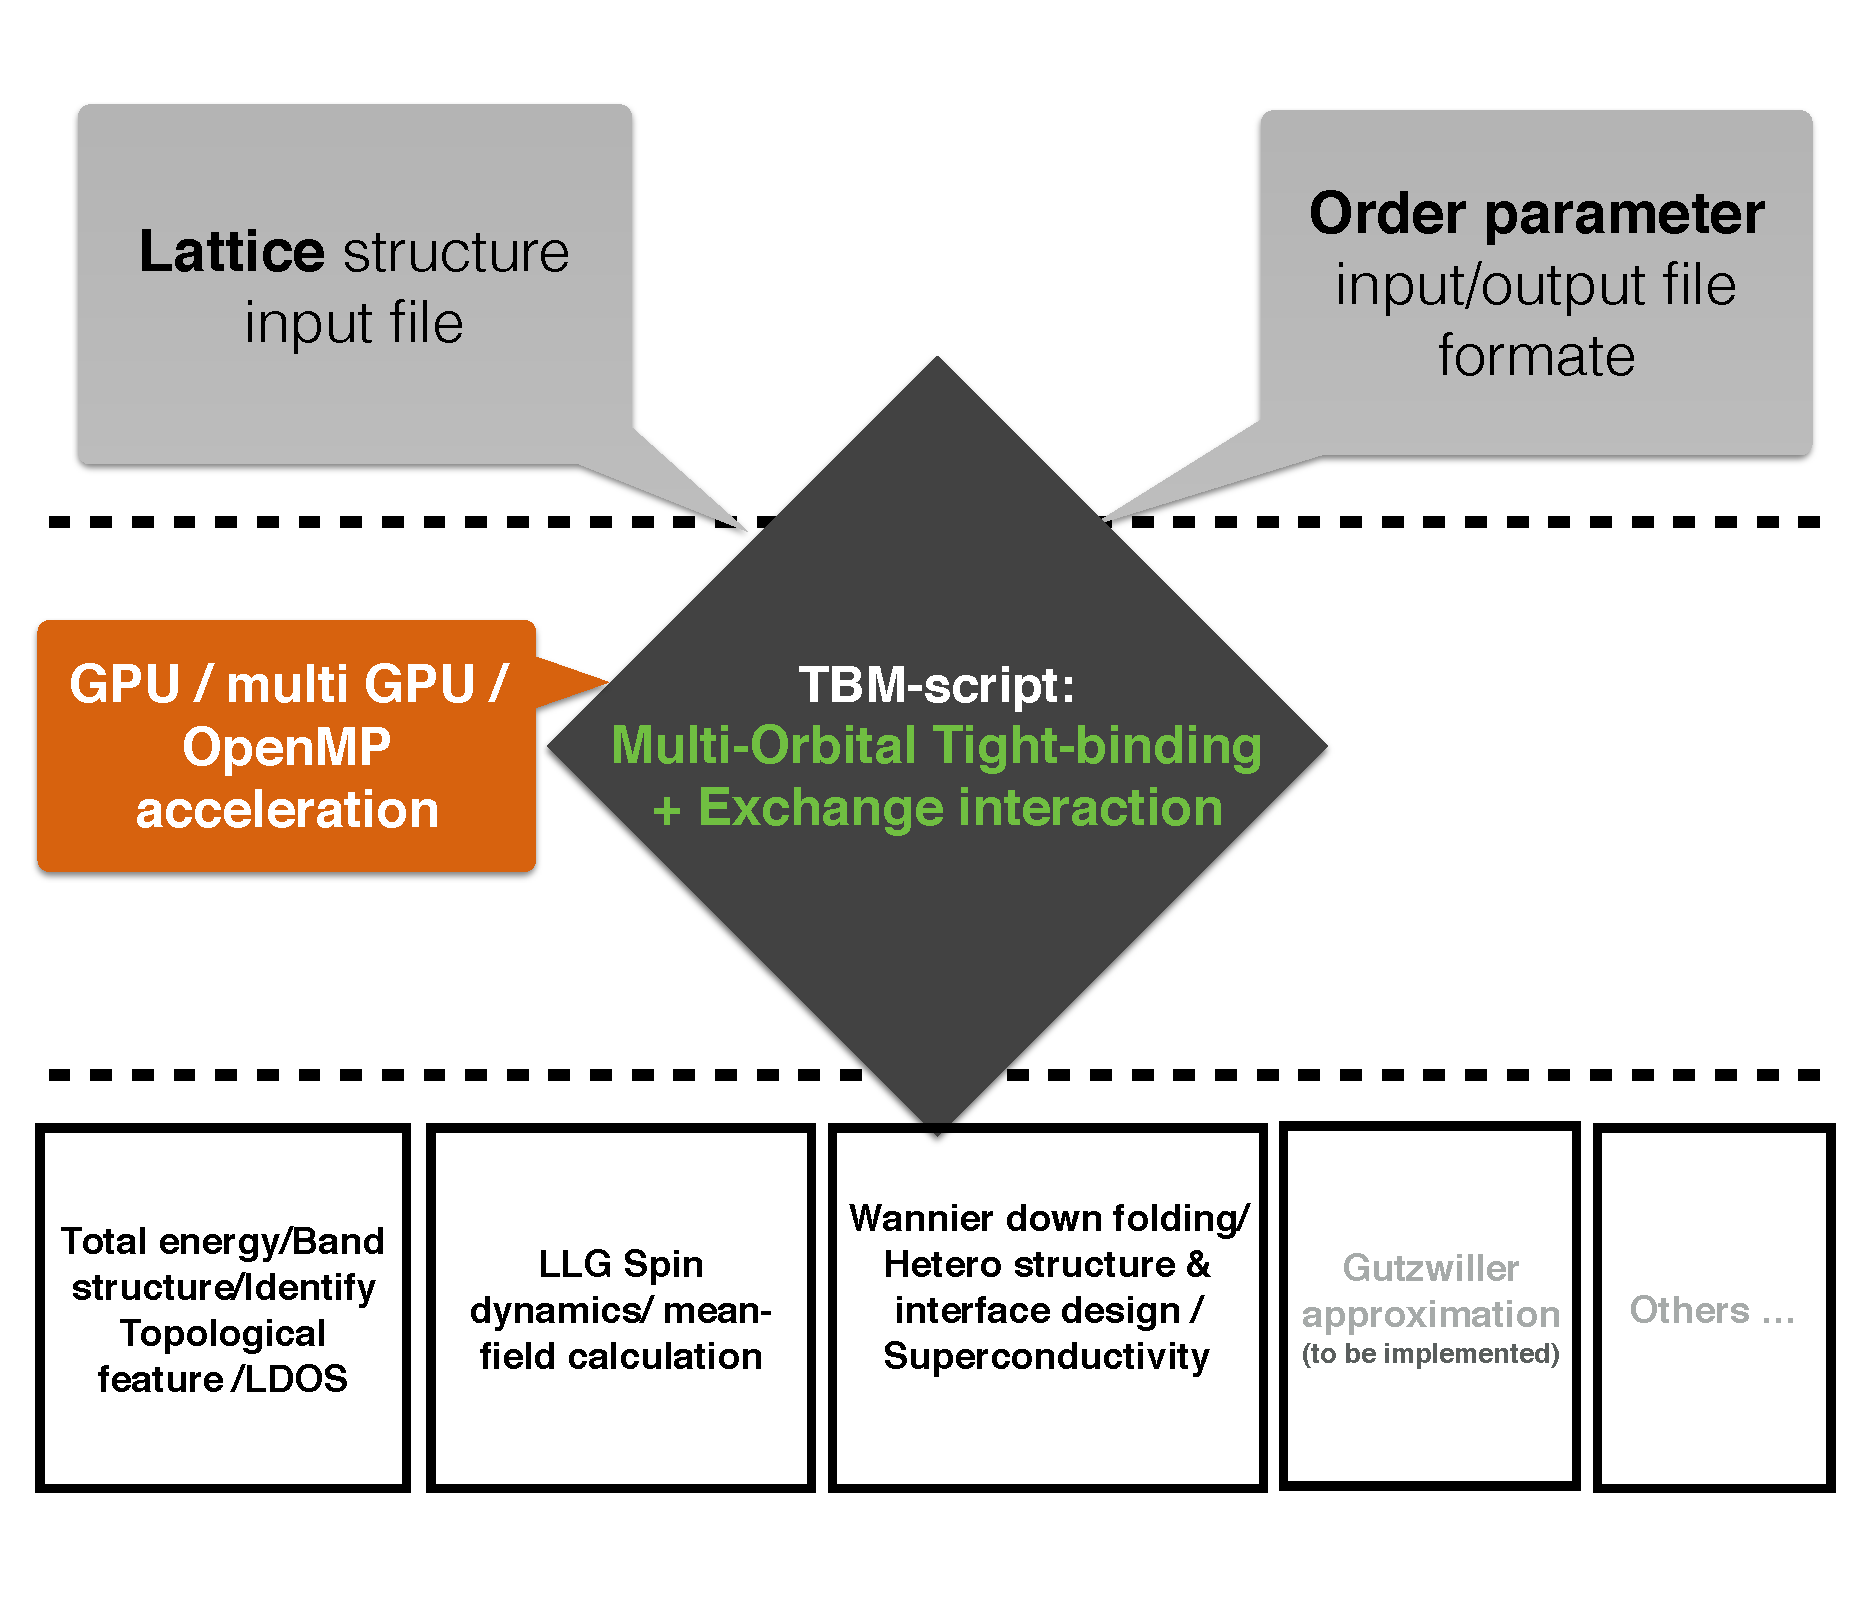
\includegraphics[scale=0.30]{./TBMCube.pdf}
%\caption{The layout of TBM$^3$ structure.}
%\label{TBMCube}
%\end{figure}

TBM$^3$ has many outstanding properties, compared to the existing solutions. Please let us list several of them as below:
\begin{itemize}
  \item \textit{Universality}.--- TBM$^3$ provides a natural way for the design and construction of hamiltonians with multi-orbital and spin degrees of freedom, 
  and investigating their electronic structures. TBM$^3$ can deal with any kind of lattice structure with different lattice symmetry groups (including symmorphic space groups and non-symmorphic space groups), any kind of lattice geometry (including bulk, ribbon, quantum dot), and any kind of dimension (from one dimension to three dimension). In the current framework, TBM$^3$ has been successful applied to a wide class of problems, for instance, transition-metal-oxide heterostructure, two-dimensional transition-metal dichalcogenides, graphene, topological insulators, and skyrmion in materials.  \\
  \item \textit{Extensibility}.--- TBM$^3$ can used as either a solver for a tight-bind model, or a postprocessing tool
with most existing ab initio or DFT packages or libraries (VASP, Wien2K, Quantum Espresso, etc.). In addition, TBM$^3$ is also ideally suited for high-throughput of materials databases for various compounds (Metweb, etc. ).
  \item \textit{High performance}.--- TBM$^3$ is constructed based on C++ language. More importantly, TBM$^3$ provides options to perform the calculations based on 
  either CPU or GPU parallel architecture. C++ combined with GPU parallel architecture accelerate the calculations in an amazing way. \\
  \item \textit{User-friendly}.---  TBM$^3$ is designed in an easy scripting way to translate the physical models (usually are written in the second quantization mathematical form) to the matrix equation for the numerical calculations. We also created a handy tool that bridges the DFT calculated parameters (the Wannier90 output file, etc.) to the TBM-scripting interface. Therefore, the model scheme and the DFT guided parameters can be smoothly combined together, without any difficulty.\\
\end{itemize}

Overall, we believe TBM$^3$ to be of particular interest to both students and senior researchers,
who can use it to explore physical properties in various materials, and build up intuition about quantum many-body problems.
TBM$^3$ was firstly applied to solve a heterostructure interface physics problem in mesoscale~\cite{YYTai01}, 
and we are looking forward for more applications with it. In the future,
we desire to include other algorithms in TBM$^3$ such as Gutzwiller approximation \cite{guziwiller}, dynamical mean-field theory \cite{dmft1,dmft2} or Monte carlo simulations \cite{qmc1,qmc2}.
This document will walk through several simple tutorial for the purpose of understanding that how TBM$^3$ works, 
and a detailed documentation of TBM$^3$ is also presented.


\clearpage




\section{Version, License, Citation and Facebook Group}
\subsection{Document version - 1.0}
TBM$^3$ is currently in version 1.0.
This document will be updated and keep the same version number with TBM$^3$ in the future.
Any future updates and correspond change log will be placed in here.

\subsection{BSD License}
TBM$^3$ is licensed under the BSD Berkeley Software Distribution.
For the usage and distribution of TBM$^3$ package, please see the ``LICENSE.txt" under the root folder of TBM$^3$.

\subsection{Citation for publication}
TBM$^{3}$  is free for academic researchs. Any publications using TBM$^{3}$  for their calculations should cite as: Yuan-Yen Tai, Wei Zhu, Hongchul Choi, and Jian-Xin Zhu, TBM$^{3}$: Tight Binding Model for Materials at Mesoscale, https://github.com/TDIV/TBM3.

\subsection{Facebook group fourm}
If you have any question or if you like to follow our future updates or if you like to give feedback to us, please join our Facebook group fourm:
\begin{center}
https://www.facebook.com/groups/858544727613583/
\end{center}

\clearpage

\section{Compile and installation}
In order to compile and install the TBM$^3$ package, one needs to pre install several C/C++ libraries in advance. Here is the steps to compile and install the TBM$^3$ package:
\begin{enumerate}
	\item Install {\bf \href{https://developer.nvidia.com/cuda-downloads}{CUDA}} driver and SDK, Ref.~\onlinecite{cuda}.
	\item Install {\bf \href{http://icl.cs.utk.edu/magma/}{MAGMA}} library, Ref.~\onlinecite{magma}.
	\item Install {\bf \href{http://www.boost.org}{BOOST}} library, Ref.~\onlinecite{boost}.
	\item Download and unpack the TBM$^3$ package, Ref.~\onlinecite{tbm}.
	\item Download and unpack {\bf \href{https://github.com/Anrris/Gramat}{GraMat}} library on Github and place it under the TBM$^3$ root folder to be named as ``Gramat", Ref.~\onlinecite{gramat}.
	\item Choose and copy one of the {\bf make.inc.xxxxx} to {\bf make.inc} under the unzipped folder.
	\item Modify {\bf make.inc} according to the library path of CUDA, MAGMA and BOOST.
	\item Type {\bf make} to compile TBM$^3$ package.
	\item If sucessfully compiled, two executable files ({\bf tbm-run} and {\bf tbm-wannier}) will be generated under the bin/ folder.
	\item Add {\bf ``/path to TBM$^3$ folder/bin/"} to the system path.
\end{enumerate}
After all, several executable files and useful python scripts can be found under the bin/ folder.
The main exectuable programs are:
\begin{itemize}
	\item {\bf tbm-run}, the main program that calculate band-structure, LDOS and solving interaction terms, etc.
	\item {\bf tbm-wannier}, the program that convert the Wannier90 input file into TBM-script formate.
\end{itemize}
And the python scripts are:
\begin{itemize}
	\item[$\circ$] {\bf tbm-band.py}, for plotting the calculated band structure.
	\item[$\circ$] {\bf tbm-kwannier.py}, for plotting the calculated Wannier center under the k-space.
	\item[$\circ$] {\bf tbm-lattice.py}, for modifying a group of atom name of the lattice input file.
	\item[$\circ$] {\bf tbm-order.py}, for modifying the order parameter I/O-file (electron occupancy, spin, four-density, etc).
\end{itemize}
Those python scripts are a set of counter part of the TBM$^3$ package to manipulate the input files.
To use these python scripts, one have to install the {\bf Numpy}, {\bf Scipy} and {\bf Matplotlib} with Python 2.7.

\clearpage

\section{TBM$^3$ Tutorial}
\subsection{Construct single orbital tight-binding model on square lattice} 
In this section, you will learn how to setup the two files: [filename].lat, and [filename].lat.tbm and generate the band structure of a given lattice and Hamiltonian.

To make a tight-binding model, the first step is to construct the lattice structure for it. 
Here we create a file named {\bf square.lat} with the following content.


\begin{lstlisting}[language=C++]
% This is a comment.
% One can use the '%' symbol to make comments
% in anywhere of the document.

#BasisVector
 1               0               0       
 0               1               0              
 0               0               1              

#OrbitalProfile
Cu        dx2-y2

#Atoms
1     0             0             0            
\end{lstlisting}
It contain three blocks:
1.{\bf \#BasisVector} describes the basis vector of the lattice. Here we have $a_1=(1,0,0)$, $a_2=(0,1,0)$ and $a_3=(0,0,1)$, 2.{\bf \#OrbitalProfile} describes which orbital you choose for the Cu atom, and 3.{\bf \#Atoms} describes all the atom positions.

Here, since we have only one atom, the coordinat for the lattice system could be arbitrary, and we set it to the origin:
\begin{lstlisting}[language=C++]
#Atoms
1     0             0             0
\end{lstlisting}
in {\bf line 14} the number `{\bf 1}' indicated that it is using the first component from the {\bf \#OrbitalProfile}.

Now, we are ready to construct the hopping terms for this lattice.
Following the name of {\bf square.lat}, we create a TBM-script named {\bf square.lat.tbm} to describe the Hamiltonian for it:
\begin{equation}
H = \sum_{i\delta, \alpha\beta\, \sigma} t_{i\alpha;i+\delta,\beta}\;\; c_{i,\alpha\sigma}^{\dagger} c_{i+\delta,\beta\sigma}.
\end{equation}

This Hamiltonian is generally for multi-orbital and multi-site hopping terms.
However, here we are going to setup up a single orbital model with only nearest neighbor hopping terms.
The following Hamiltonian is actually considered:
$H = t\;\; \sum_{i,\delta\in NN}\;\; c_{i,\sigma}^\dagger c_{i+\delta,\sigma}$,
and the corresponding {\bf square.lat.tbm} script is:
\begin{lstlisting}[language=C++]
#Parameters
t  =  -1

#CoreCharge
Cu  >  1

#Hamiltonian
hopping  >  Cu:Cu:+1+0+0  1:1  > t
hopping  >  Cu:Cu:-1+0+0  1:1  > t
hopping  >  Cu:Cu:+0+1+0  1:1  > t
hopping  >  Cu:Cu:+0-1+0  1:1  > t
\end{lstlisting}

the {\bf square.lat.tbm} script has three blocks to describe the model:
\begin{itemize}
\item {\bf\#Parameters} setup the value for the hopping term.\\
\item {\bf\#CoreCharge} setup the core charge for the Cu atom, the total charge value will be balanced with the itinerant electrons of Cu.\\
\item {\bf\#Hamiltonian} setup the hopping terms.\\
\end{itemize}
Inside the {\bf\#Hamiltonian} block,
\begin{lstlisting}[language=C++]
hopping  >  Cu:Cu:+1+0+0  1:1  > t	
\end{lstlisting}
,describes the hopping, t, through the Cu-Cu bonding, $\delta=(1,0,0)$, for any sites from orbital-1(dx2-y2) to orbital-1 (dx2-y2).

\begin{figure}
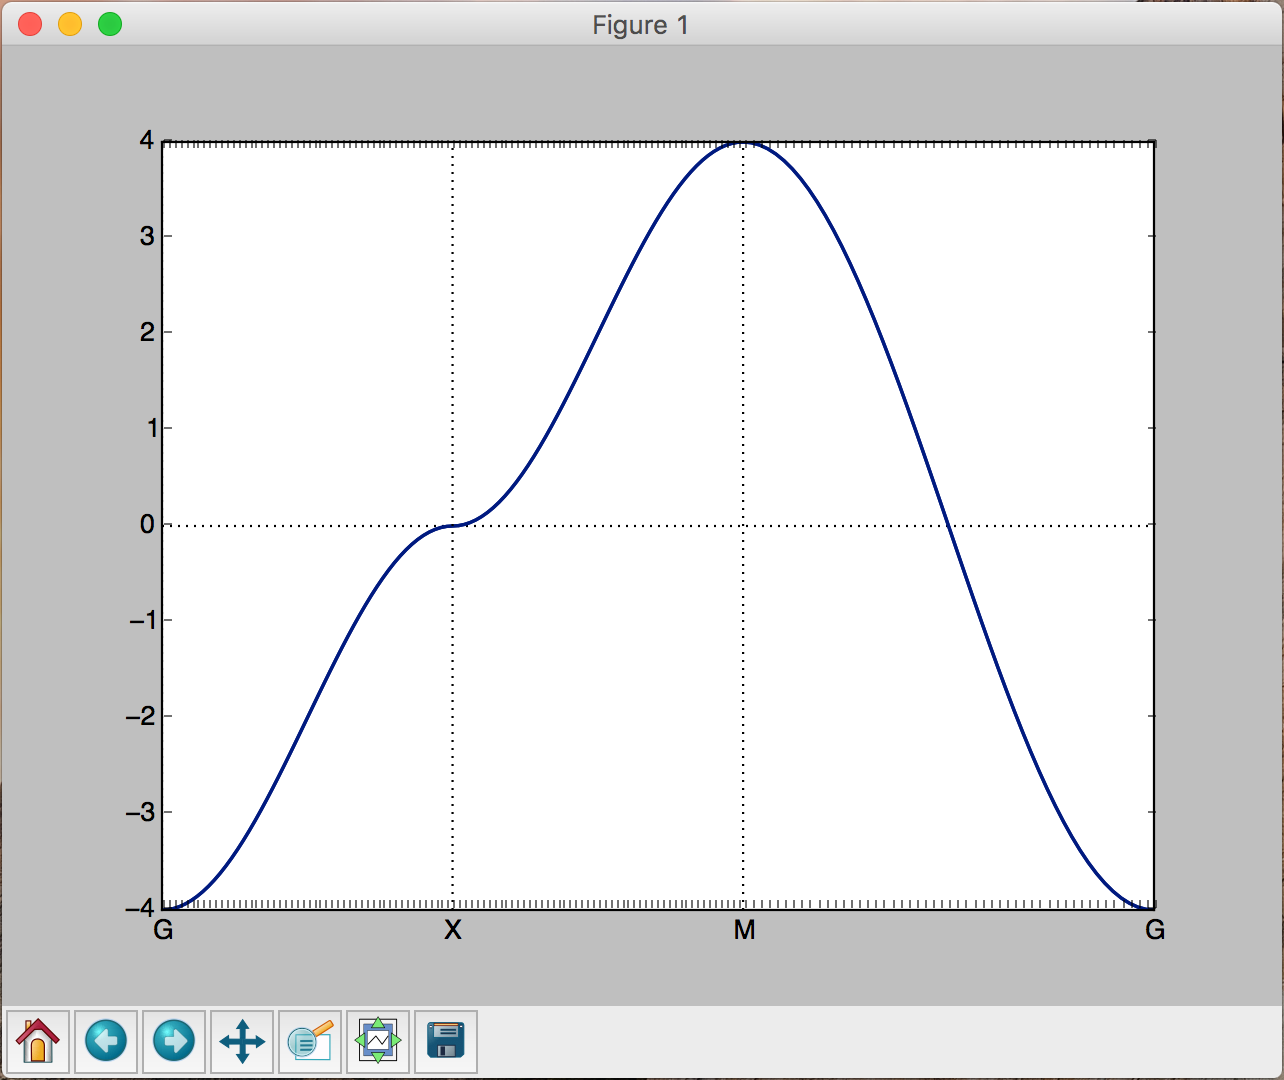
\includegraphics[scale=0.30]{./figs/fig01-01.png}
\caption{The calculated band structure of a simple 2D square lattice.}
\label{fig01-01}
\end{figure}

Now, we have done the setup of Hamiltonian (hopping terms) for our model.
However, in order to get some physical properties calculated, we have to add few more lines in the {\bf square.lat.tbm} script:
\begin{lstlisting}[language=C++]
#KPointPath
G      0     0     0    
X      0.5   0     0    
M      0.5   0.5   0    
G      0     0     0    

#Parameters
isCalculateMu   = 1
isCalculateBand = 1
Nb = 4,4,1

spin = "on"
space = "normal"
bondRadius = 1

t  =  -1

#CoreCharge
Cu  >  1

#Hamiltonian
hopping  >  Cu:Cu:+1+0+0  1:1  > t
hopping  >  Cu:Cu:-1+0+0  1:1  > t
hopping  >  Cu:Cu:+0+1+0  1:1  > t
hopping  >  Cu:Cu:+0-1+0  1:1  > t
\end{lstlisting}
In above, the {\bf\#KPointPath} block describes how we setup the k-poin paths based on the Bravais vector.
For example, in the {\bf square.lat.tbm} file,:
\begin{lstlisting}[language=C++]
X      0.5   0     0
\end{lstlisting}
means setup a k-point path for, $X = 0.5\times{b_1}+0\times{b_2}+0\times{b_3}$.
The new parameter {\bf isCalculateMu = 1} tells TBM$^3$ to calculate the chemical potential automatically, and {\bf isCalculateBand = 1} tells TBM$^3$ to calculate the band structure according to the {\bf\#KPointPath} block , and {\bf Nb = 4,4,1} tells TBM$^3$ how many k-points to be used for the calculation of chemical potential (Mu).

Here the model spin is turned "on" according to {\bf spin = "on"}, and it is under "normal" space due to {\bf space = "normal"}.
The {\bf bondRadius = 1} tells $TBM^3$ searching for the near by atoms within that range.

Finally, under the terminal, execute the "tbm-run" program:
\begin{lstlisting}[language=C++]
\$> tbm-run square.lat

Starting...

>> Calculating the chemical potential, Mu.
 Mu         Dest e-den True e-den total_n_diff
  0          1         -  1         = -5.18168e-10

With spin:on
And space:normal
Total electron count: 1

>> Calculating the Band structure.
Finished.
\end{lstlisting}
This will generate a new file name "square.lat.ban" that contains the band structure of the square lattice.
You can plot this band structure in using "tbm-band.py", see Fig.~\ref{fig01-01}:
\begin{lstlisting}[language=C++]
\$> tbm-band.py square.lat.ban	
\end{lstlisting}


\subsection{Graphene models}
\subsubsection{Construct graphene model and its band structure} 
In this section, you will learn how to constructure the band structure of a single-layered graphene. You will also learn how to generate a super lattice within the 
TBM$^3$ framework. Finally, you will learn how to create the edge band structure of the open boundary graphene super lattice.
We begin with the two-sub-atom input file of graphene. Here, we choose a name {\bf graphene-honeycomb.lat} for it:

\begin{lstlisting}[language=C++]
#BasisVector
 1.5             0.866025        0              
 1.5            -0.866025        0              
 0               0               1              

#OrbitalProfile
C1        pz        
C2        pz        

#Atoms
1     0        0       0.5            
2     1        0       0.5    	
\end{lstlisting}

Here, we can enter the following commend to generate a vesta file for the viewing of the lattice structure,

\begin{lstlisting}[language=C++]
\$> tbm-run graphene-honeycomb.lat -ovesta	

Convert to the VESTA file formate:honeycomb.lat.vesta

Finished.
\end{lstlisting}
Therefore, you can use the \href{http://jp-minerals.org/vesta/en/}{VESTA} program to view it, see Fig.~\ref{fig01-02}.

\begin{figure}
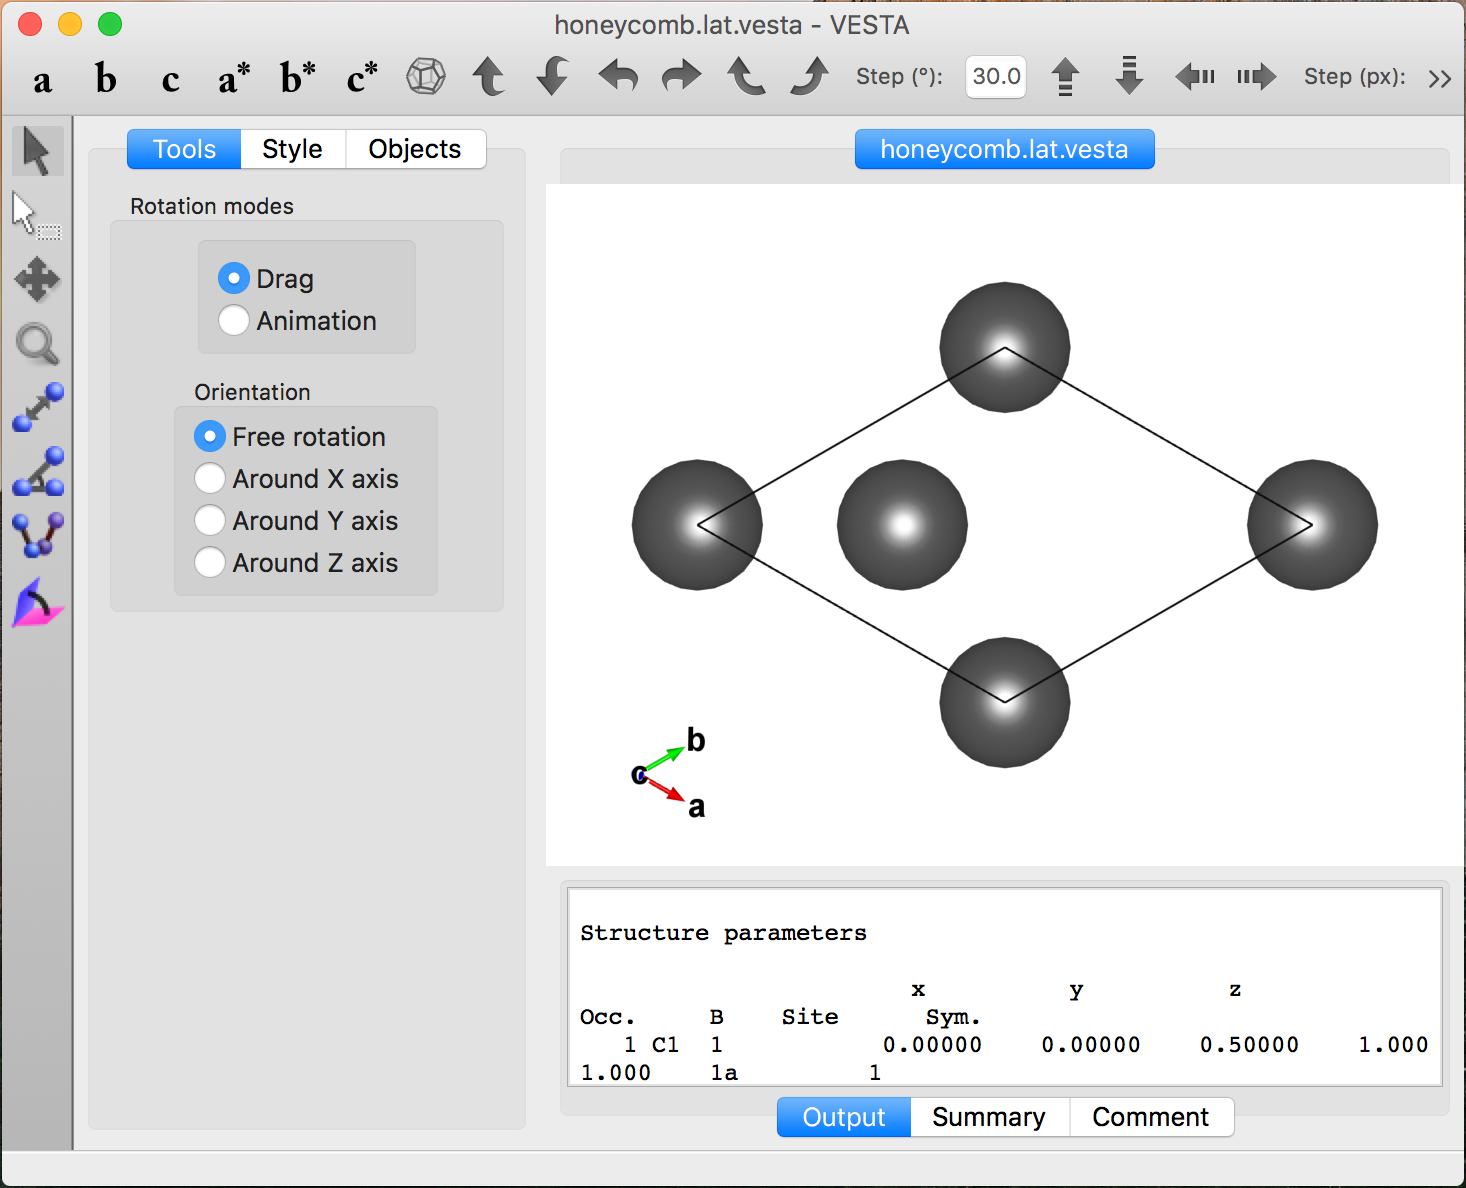
\includegraphics[scale=0.30]{./figs/fig01-02.png}
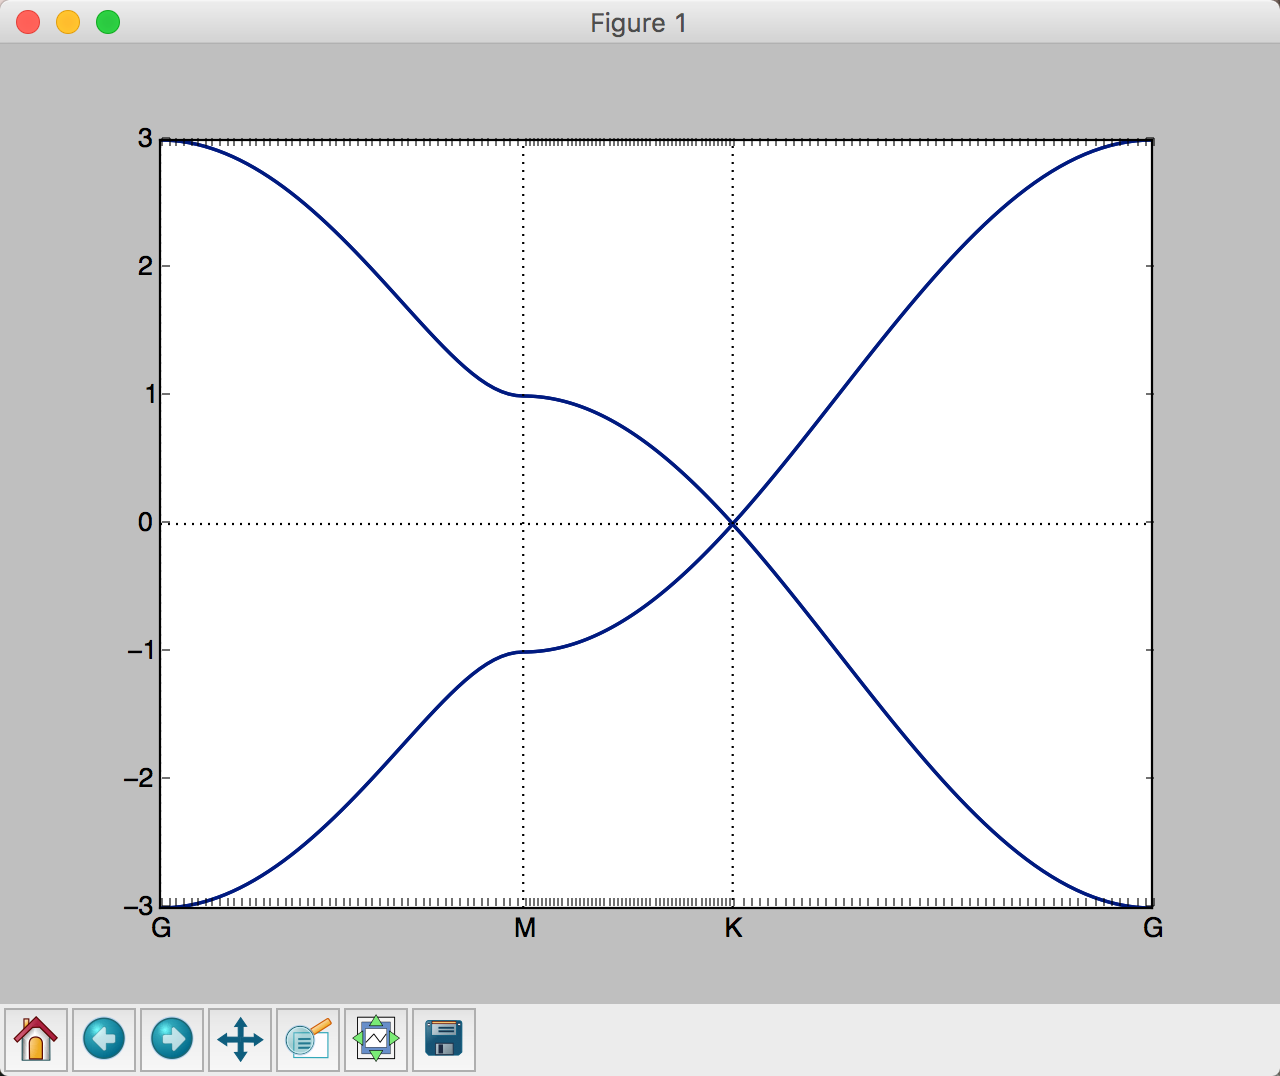
\includegraphics[scale=0.332]{./figs/fig01-03.png}
\caption{VESTA generated graphene lattice structure (left).
Band structure of graphene (right).}
\label{fig01-02}
\end{figure}

Now, use the following TBM-script for the construction of the graphene hopping terms ({\bf graphene-honeycomb.lat.tbm}):

\begin{lstlisting}[language=C++]
#KPointPath
G      0     0     0    
M      0.5   0     0    
K      0.666 0.333 0    
G      0     0     0    

#Parameters
isCalculateMu = 1
isCalculateBand = 1

Mu = 0
spin = "on"
space = "normal"
Nb = 4,4,1
bondRadius = 2

t1 = 1

#CoreCharge
C1	> 1
C2	> 1

#BondVector 0
 1.0                 0.0                 0.0                
-0.5                 0.866025403784      0.0                
-0.5                -0.866025403784      0.0                  

#Hamiltonian
hoppingHc > C1:C2:+1+0+0# 1:1 >  t1
hoppingHc > C1:C2:+0+1+0# 1:1 >  t1
hoppingHc > C1:C2:+0+0+1# 1:1 >  t1
hoppingHc > C2:C1:+1+0+0# 1:1 >  t1
hoppingHc > C2:C1:+0+1+0# 1:1 >  t1
hoppingHc > C2:C1:+0+0+1# 1:1 >  t1

\end{lstlisting}

In this script, we have introduced a new block {\bf \#BondVector 0}.
The use of this block is to simplify the construction of the hopping bond of the neighbor of C1 or C2 atoms.
Therefore, this bond description {\bf C1:C2:+0+1+0\#} is in present of {\bf \#BondVector 0} and it is exactly the same as {\bf C1:C2:-0.5+0.866025403784+0} in cartesian coordinates. 
There is another new keyword {\bf hoppingHc} under the {\bf \#Hamiltonian} block.
It means to generate a ``hermitian conjugate" hopping of the hopping expression.

Finally, following previous steps, you can generate and visualize the bulk band structure of graphene, see Fig.~\ref{fig01-03}.


\subsubsection{Construct graphene model with open boundary conditions} 
In this section, you will learn how to setup the open boundary condition for a single-layered graphene, and you will learn how to create the edge band structure of the open boundary graphene super lattice.

Graphene has two basic types of boundary: 1. Zigzag and 2. Armchair. In order to setup for this geometry, in the lattice input file, we need to change the {\bf \#BasisVecter} in orthogonal basis and add more sub-atoms in {\bf \#Atoms}.
Here we create {\bf graphene-orthogonal.lat}

\begin{lstlisting}[language=C++]
#BasisVector
 3               0               0              
 0               1.73205         0              
 0               0               1              

#OrbitalProfile
C1        pz        
C2        pz        

#Atoms
2     0.5          0.866025      0.5            
1     1            0             0.5            
2     2            0             0.5            
1     2.5          0.866025      0.5            

\end{lstlisting}

By using this $TBM^3$ operation {\bf\$ tbm-run graphene-orthogonal.lat -ovesta}, you can view the lattice structure in VESTA.

\begin{figure}
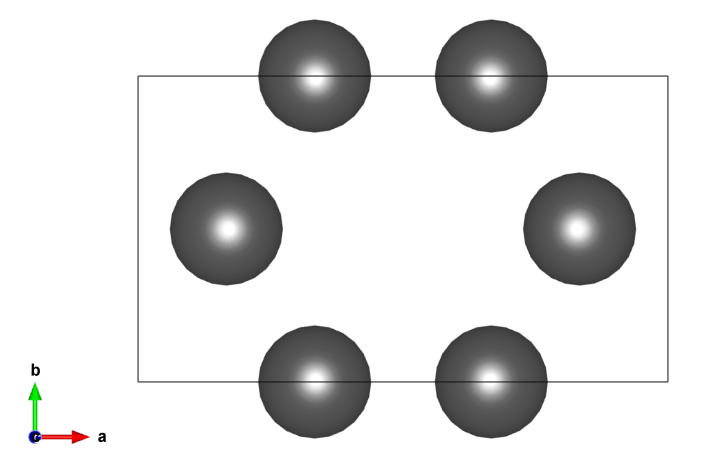
\includegraphics[scale=0.1]{./figs/fig01-04.png}
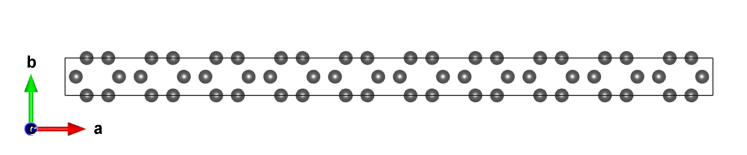
\includegraphics[scale=0.35]{./figs/fig01-05.png}
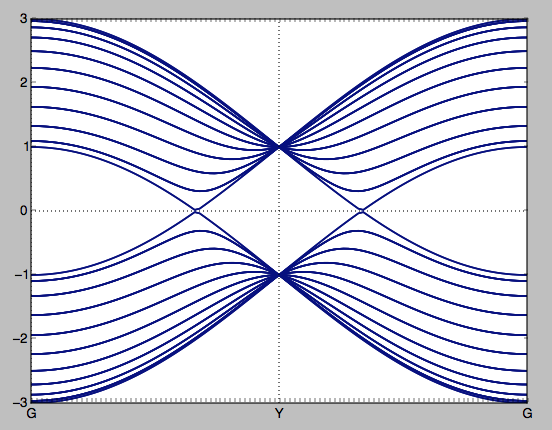
\includegraphics[scale=0.13]{./figs/fig01-06.png}
\caption{Lattice structure of ``graphene-orthogonal.lat" (left).
Expanded graphene-orthogonal lattice (middle).
The zigzag close bounday band structure (right).}
\label{fig01-03}
\end{figure}

Now, we can use the {\bf -expand} operation of $TBM^3$ to generate a supercell lattice.
\begin{lstlisting}[language=C++]
\$> tbm-run  graphene-orthogonal.lat -expand 10 1 1	

Expanding the lattice of 'graphene-orthogonal.lat' to a larger lattice.

>>>'graphene-orthogonal.10x1x1.lat'
Finished.
\end{lstlisting}
This operation tells $TBM^3$ to generate a expanded lattice based on {\bf graphene-orthogonal.lat}, and it is repeating along $a_1$ direction for $10$ times ($a_2$ and $a_3$ are repeated $1$ time, meaning, not repeating).
It automatically generated {\bf graphene-orthogonal.10x1x1.lat} and {\bf graphene-orthogonal.10x1x1.lat.tbm} according to the previous one.

We can check its band structure along the $a_2$ direction by setting the {\bf \#KPointPath} inside the ``graphene-orthogonal.10x1x1.lat.tbm" file:

\begin{lstlisting}[language=C++]
#KPointPath
G      0     0     0    
Y      0  	 0.5   0    
G      0     0     0    
\end{lstlisting}


Now, we are ready to create the Zigzag open boundary for the system by manually setting a larger lattice constant along $a_1$ direction inside the {\bf graphene-orthogonal.10x1x1.lat} file:

\begin{lstlisting}[language=C++]
#BasisVector
 34              0               0              
 0               1.73205         0              
 0               0               1         
\end{lstlisting}

\begin{figure}
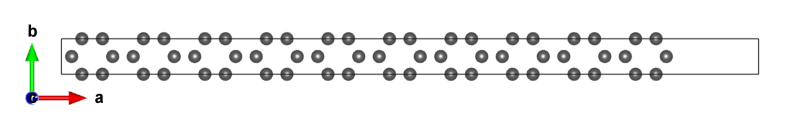
\includegraphics[scale=0.35]{./figs/fig01-07.png}
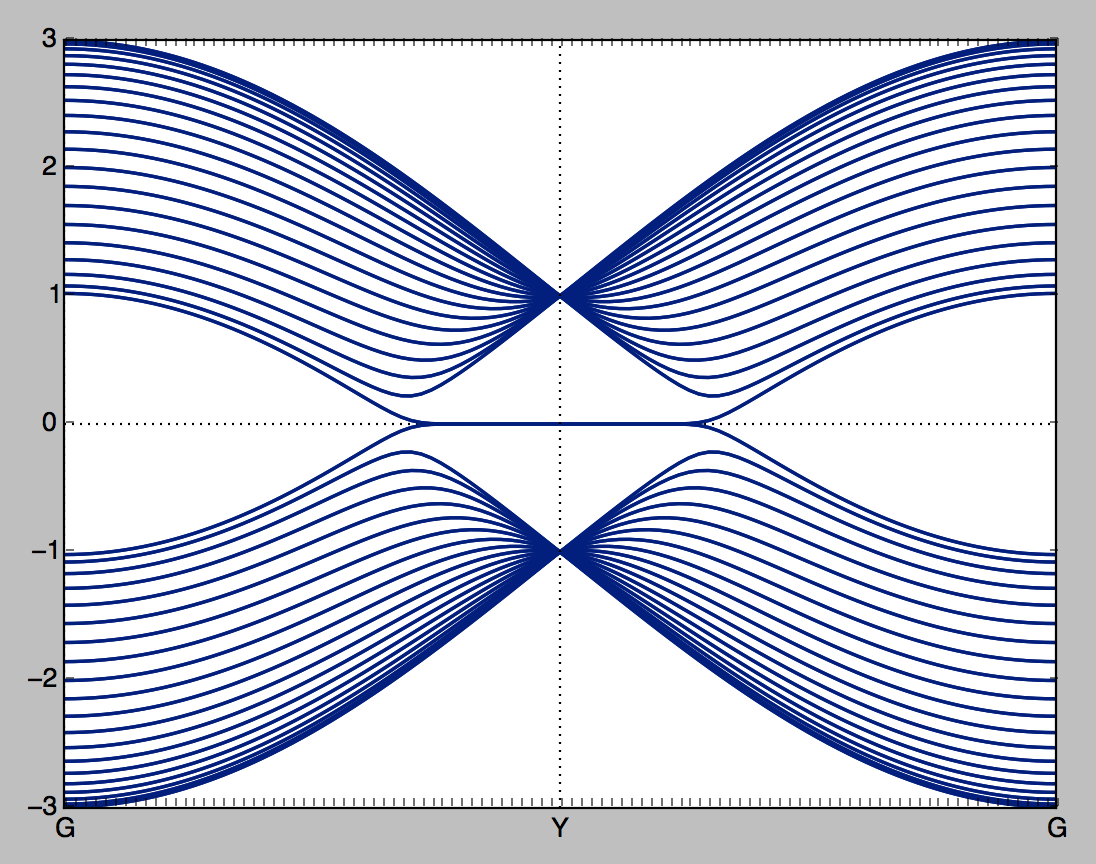
\includegraphics[scale=0.12]{./figs/fig01-08.png}
\caption{The zigzag open bounday lattice (left), and its band structure (right).}
\label{fig01-03}
\end{figure}

So far, we've presented how to create the open boundary conditions for the Zigzag edge. One can pratice on creating the Armchair edge and plot its edge band structure.

\subsubsection{Setup Haldane and Kane \& Mele model for graphene} 
Haldane introduced a imaginary hopping, $i\times t_{AH}\; \sum_{i,\delta\in 2NN} \;c_{i}^\dagger c_{i+\delta}$, to the second nearest neighbor (2NN) of graphene and created the anomalous Hall effect.
Here are two ways to access the 2NN bond: (1.) using the linear combination of the nearest neighbor bonding, and (2.) by defining a new {\bf \#BondVect} label.
Here, you will learn method (2.) in the following:

\begin{lstlisting}[language=C++]
#BondVector 1
 1.5       -0.8660254  	0.0
 0.         1.73205081  0.0
-1.5       -0.8660254  	0.0
\end{lstlisting}

The above block named {\bf \#BondVector 1} is the new bonding relations that we defined for the 2NN bond.
After all, we can easily construct this term by adding the following lines inside the {\bf \#Hamiltonian} block of "*.lat.tbm" file:

\begin{lstlisting}[language=C++]
#BondVector 0
 1.0                 0.0                 0.0                
-0.5                 0.866025403784      0.0                
-0.5                -0.866025403784      0.0  

#BondVector 1
 1.5       -0.8660254  	0.0
 0.         1.73205081  0.0
-1.5       -0.8660254  	0.0

#Hamiltonian
hoppingHc > C1:C2:+1+0+0# 1:1 >  t1
hoppingHc > C1:C2:+0+1+0# 1:1 >  t1
hoppingHc > C1:C2:+0+0+1# 1:1 >  t1
hoppingHc > C2:C1:+1+0+0# 1:1 >  t1
hoppingHc > C2:C1:+0+1+0# 1:1 >  t1
hoppingHc > C2:C1:+0+0+1# 1:1 >  t1

% 2NN hopping (Haldane model)
hoppingHc > C1:C1:+1+0+0#1 1:1 > (0, 1)*t_AH
hoppingHc > C1:C1:+0+1+0#1 1:1 > (0, 1)*t_AH
hoppingHc > C1:C1:+0+0+1#1 1:1 > (0, 1)*t_AH
hoppingHc > C2:C2:+1+0+0#1 1:1 > (0,-1)*t_AH
hoppingHc > C2:C2:+0+1+0#1 1:1 > (0,-1)*t_AH
hoppingHc > C2:C2:+0+0+1#1 1:1 > (0,-1)*t_AH

\end{lstlisting}
To access the elements of {\bf \#BondVector 1} we have to indicate that after the {\bf \#} symbol at the correspond terms such as:

\begin{lstlisting}[language=C++]
hoppingHc > C1:C1:+1+0+0#1 1:1 > (0, 1)*t_AH.
\end{lstlisting}

This is the setup of a "Chern" topological insulator with Chern number $=\pm 1$ of the spinless system, and $\pm 2$ for spinful one.

Later on, Kane \& Mele extended Haldane's model to the spin degree of freedom, and yield the imaginary hopping has a sign change for different spin part, $i\times t_{AH}\; \sum_{i,\delta\in 2NN,\sigma} \sigma \;c_{i,\sigma}^\dagger c_{i+\delta,\sigma}$, this term can be described in the following way:

\begin{lstlisting}[language=C++]
% 2NN hopping (K M model)
bondHc > C1:C1:+1+0+0#1 1u:1u > (0, 1)*t_AH
bondHc > C1:C1:+0+1+0#1 1u:1u > (0, 1)*t_AH
bondHc > C1:C1:+0+0+1#1 1u:1u > (0, 1)*t_AH
bondHc > C2:C2:+1+0+0#1 1u:1u > (0,-1)*t_AH
bondHc > C2:C2:+0+1+0#1 1u:1u > (0,-1)*t_AH
bondHc > C2:C2:+0+0+1#1 1u:1u > (0,-1)*t_AH

bondHc > C1:C1:+1+0+0#1 1d:1d > (0,-1)*t_AH
bondHc > C1:C1:+0+1+0#1 1d:1d > (0,-1)*t_AH
bondHc > C1:C1:+0+0+1#1 1d:1d > (0,-1)*t_AH
bondHc > C2:C2:+1+0+0#1 1d:1d > (0, 1)*t_AH
bondHc > C2:C2:+0+1+0#1 1d:1d > (0, 1)*t_AH
bondHc > C2:C2:+0+0+1#1 1d:1d > (0, 1)*t_AH

\end{lstlisting}

Here, we introduced a new keyword {\bf bondHc} for the {\bf\#Hamiltonian} block. The meaning of {\bf bond} is similar to hoppingHc, however, it is a spin-dependent operation. Therefore, you can use it for designing the spin-dependent hopping operations.
 
Under this setup, the Chern number is zero, but it can be identified with $Z_2$ index. However, in both cases, the bulk band and edge band structure looks exactly the same. The following figures are calculated by setting $t_{AH} = 0.1$.

\begin{figure}
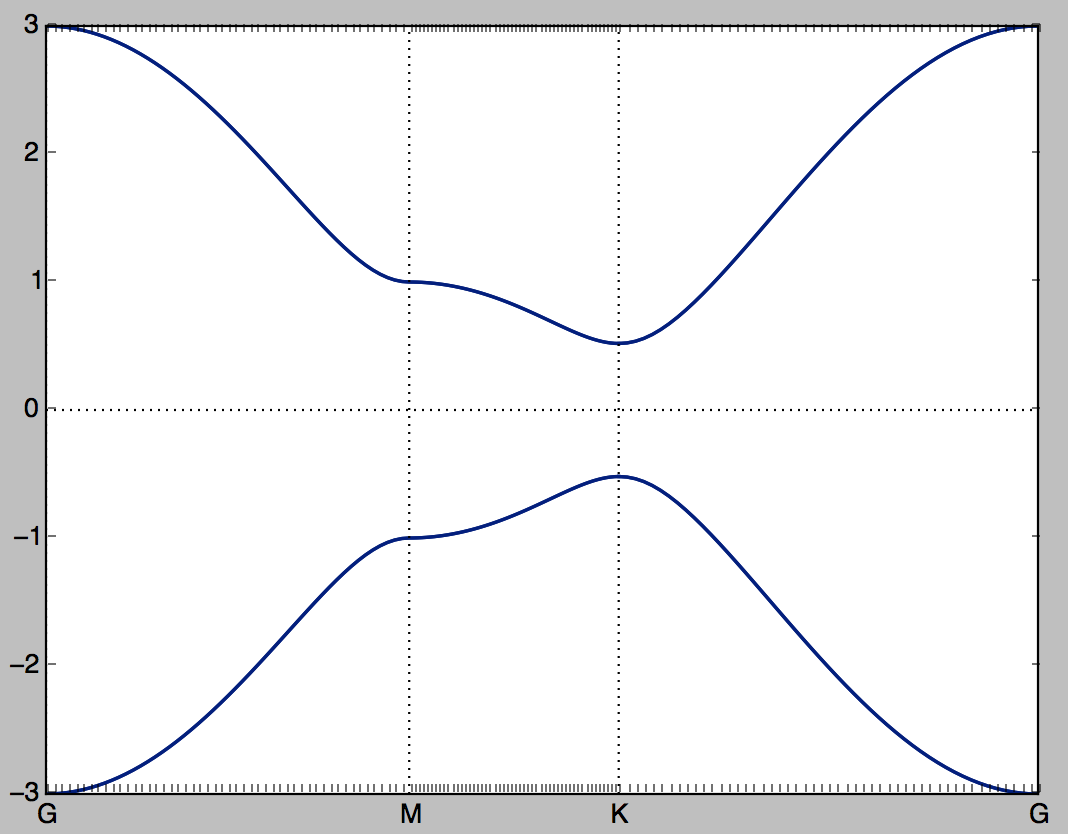
\includegraphics[scale=0.15]{./figs/fig01-09.png}
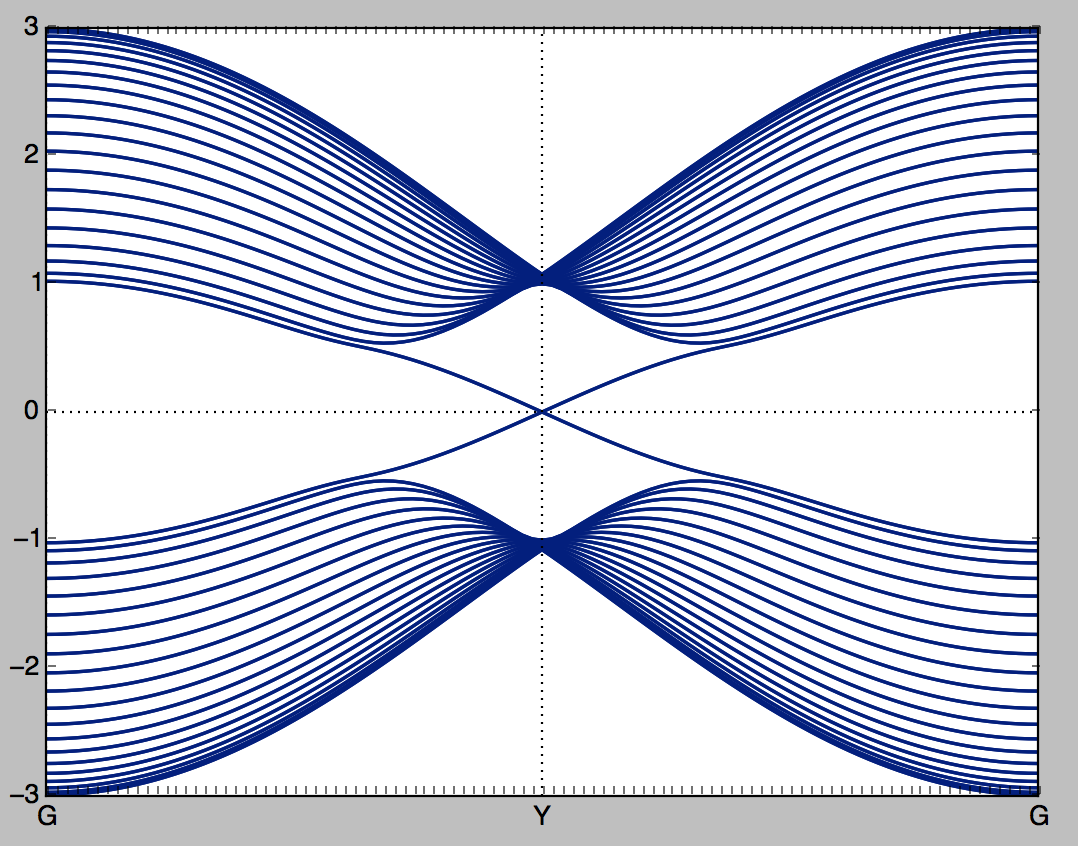
\includegraphics[scale=0.15]{./figs/fig01-10.png}
\caption{The gap structure of the graphene model with flux terms (left).
The Dirac-cone of the zigzag edge state (right).}
\label{fig01-03}
\end{figure}

\clearpage

\subsection{Construct multi-orbital Kondo lattice model} 
Here we will construct the perovskite lattice structure of the BiFeO$_3$ (BFO) compound in the cubic coordinate.
The lattice constant is set to be ``1". The readers might need to find out the experimental lattice constant by themselves. 
The following lattice input file, ``BFO.lat", describe the single unit cell BFO structure,
\begin{lstlisting}[language=C++]
#BasisVector
 1               0               0              
 0               1               0              
 0               0               1              

#OrbitalProfile
Bi        
Fe        dx2-y2    dz2       
O         px        
O         py        
O         pz        

#Atoms
1     1               1               1              
2     0.5             0.5             0.5            
3     1               0.5             0.5            
4     0.5             1               0.5            
5     0.5             0.5             1        
\end{lstlisting}
and the following TBM-script, ``BFO.lat.tbm", describes the Hamiltonian and the correspond operations that we need,
\begin{lstlisting}[language=C++]
#KPointPath
G      0     0     0    
X      0.5   0     0    
M      0.5   0.5   0    
U      0.5   0.5   0.5  
G      0     0     0    

#BondVector 0
 0.5             0               0              
 0               0.5             0              
 0               0               0.5            

#CoreCharge
Bi	> 3
Fe	> 5
O	> 0

#Init
Fe   cspin  > 0,0,1
Fe   den    > 2
O    den    > 1

#Parameters
isCalculateMu	= 1
isCalculateVar 	= 1
isCalculateBand	= 1

spin		= "on"
space		= "normal"
Nb			= 3,3,3
LLG_dt		= 0.1
MF_mix		= 0.1
LLG_diff	= 0.000001
MF_diff		= 0.001
bondRadius	= 3

Mu			= 0
Temperature	= 0.0001
Jh			= 2
tdp			= 1.0
tpp			= 0.5

#Hamiltonian
hundSpin  > Fe 1 > @:cspin * Jh 
hundSpin  > Fe 2 > @:cspin * Jh 

orbital > O 1	> -4

hoppingHc > Fe:O:+1+0+0# 1:px >  0.5  		* tdp
hoppingHc > Fe:O:+0+1+0# 1:py >  0.5  		* tdp
hoppingHc > Fe:O:+0+0+1# 1:pz > -1.0  		* tdp
hoppingHc > Fe:O:-1+0+0# 1:px > -0.5  		* tdp
hoppingHc > Fe:O:+0-1+0# 1:py > -0.5  		* tdp
hoppingHc > Fe:O:+0+0-1# 1:pz >  1.0  		* tdp
hoppingHc > Fe:O:+1+0+0# 2:px > -0.866025	* tdp
hoppingHc > Fe:O:+0+1+0# 2:py >  0.866025	* tdp
hoppingHc > Fe:O:+0+0+1# 2:pz >  0.0		* tdp
hoppingHc > Fe:O:-1+0+0# 2:px >  0.866025	* tdp
hoppingHc > Fe:O:+0-1+0# 2:py > -0.866025	* tdp
hoppingHc > Fe:O:+0+0-1# 2:pz > -0.0		* tpd

% O-O bond hopping terms
hopping > O:O:+1+1+0# 1:1 >  1 * tpp
hopping > O:O:+1-1+0# 1:1 > -1 * tpp
hopping > O:O:-1+1+0# 1:1 > -1 * tpp
hopping > O:O:-1-1+0# 1:1 >  1 * tpp
hopping > O:O:+1+0+1# 1:1 >  1 * tpp
hopping > O:O:+1+0-1# 1:1 > -1 * tpp
hopping > O:O:-1+0+1# 1:1 > -1 * tpp
hopping > O:O:-1+0-1# 1:1 >  1 * tpp
hopping > O:O:+0+1+1# 1:1 >  1 * tpp
hopping > O:O:+0+1-1# 1:1 > -1 * tpp
hopping > O:O:+0-1+1# 1:1 > -1 * tpp
hopping > O:O:+0-1-1# 1:1 >  1 * tpp
\end{lstlisting}

Above ``BFO.lat.tbm" file describes the following Hamiltonian,
\begin{equation}
\begin{aligned}
\label{Kondo}
H = & \sum_{Ib\, m\, s} t^{(pd)}_{Ib} O^{1}_{m\, b}\; ( d^\dagger_{I\, m\, s} p_{Ibs} + p^\dagger_{Ibs} d_{I\, m\, s})
		+  \sum_{I,b\neq c,s}t^{(pp)}_{Ibc} O^{2}_{b-c} \;p^\dagger_{Ibs} p_{Ics}
        -  \sum_{I\, m\, ss'} J^H_I\, \vec S_I \cdot \vec \sigma_{ss'} d^\dagger_{I\, m\, s} d_{I\, m\, s'}
        +  \sum_i (\varepsilon_i - \mu)n_i,
\end{aligned}
\end{equation}
is taken from Ref.~\onlinecite{YYTai01}.
Notice that, the long-range Coulomb interaction is not considered in this tutorial.
In Eq.~\ref{Kondo} the $J^H_I$ term describes the coupling of classical t$_{2g}$ spin to the itinerant e$_g$ electrons.
In this model, we calculate the force term of each Fe-spin, $\partial H/\partial \vec S_I$, and using the LLG-dynamics to optimize the spin structure.
In order to do that, we have to generate a larger real-space lattice for our calculation,
\begin{lstlisting}
\$> tbm-run BFO.lat -expand 2 2 2
\end{lstlisting}
and initialize the spin structure for our calculation in using the {\bf \#Init} block of line 34,
\begin{lstlisting}
\$> tbm-run BFO.2x2x2.lat -init
\end{lstlisting}
Finally, we have generated the ``BFO.2x2x2.lat.ord",
\begin{lstlisting}
>>> 0   1    Bi   [[ 0.5   0.5   0.5 ]]
>>> 1   2    Fe   [[ 0     0     0   ]]
 @:den = 2
 @:cspin = 0,0,1
>>> 2   3    O    [[ 0.5   0     0   ]]
 @:den = 1
>>> 3   4    O    [[ 0     0.5   0   ]]
 @:den = 1
>>> 4   5    O    [[ 0     0     0.5 ]]
 @:den = 1
...
...
\end{lstlisting}
The ``BFO.2x2x2.lat.ord" describe each Fe atoms has 2 electron occupation with the classical spin pointing in positive $z$-direction and each O atoms has 1 electron occupation, Fig.~\ref{fig01-11}.
However, if all of the spins are parallel in the initial state, the resulting calculated forces will be zero.
Therefore, we can edit the orders of ``BFO.2x2x2.lat.ord" and manually making some spins unparallel to each other (Please find out how to manipulate the order parameters in next section {\bf ``TBM$^3$ Document"}).

\begin{figure}
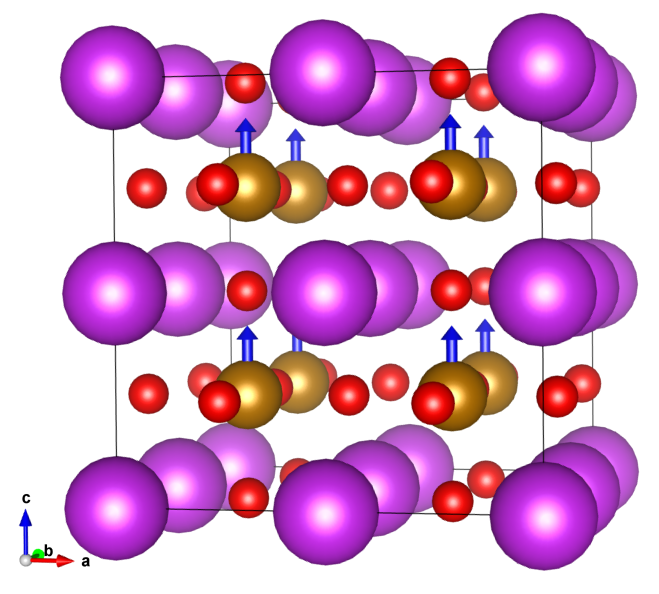
\includegraphics[scale=0.15]{./figs/fig01-11.png}
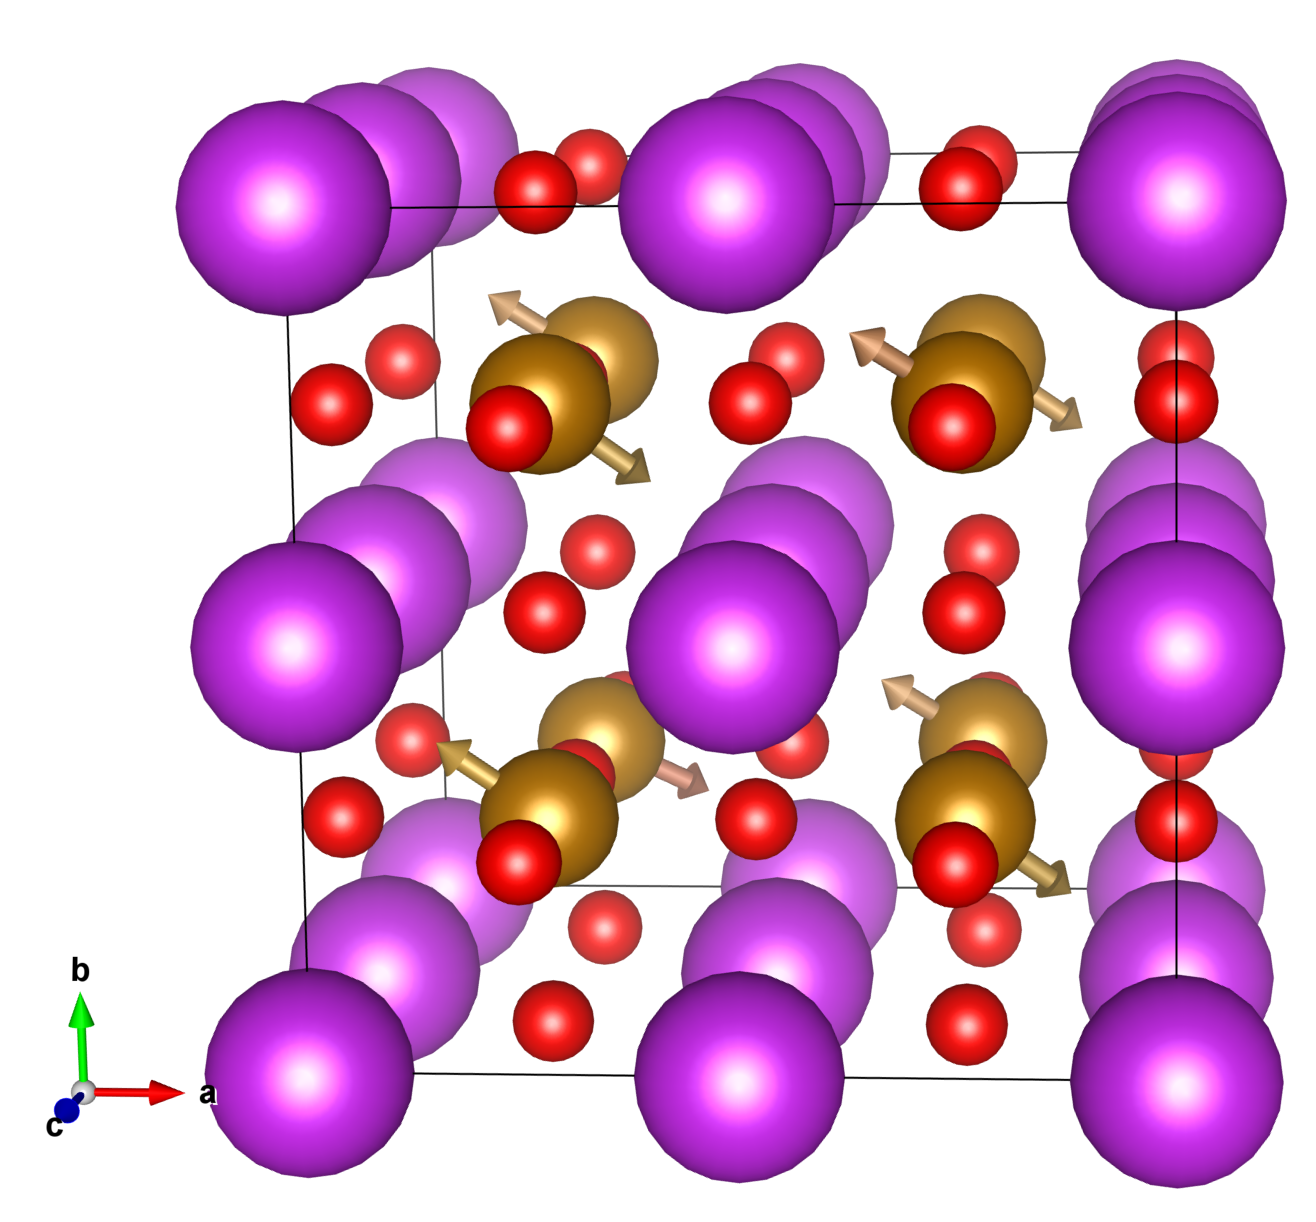
\includegraphics[scale=0.15]{./figs/fig01-12.png}
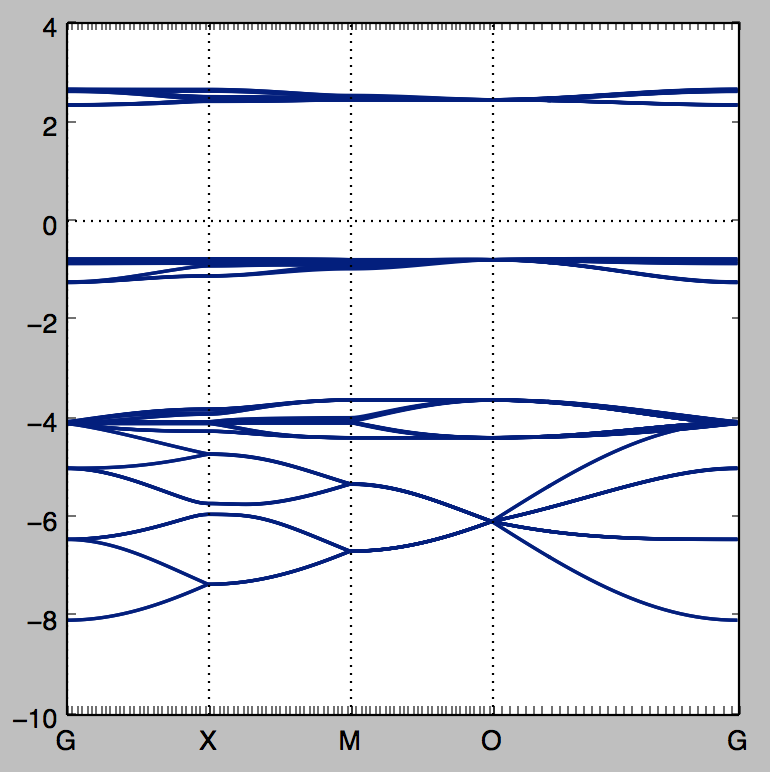
\includegraphics[scale=0.22]{./figs/fig01-13.png}
\caption{Lattice structure and the initial classical spin order of a 2x2x2 BFO lattice (left).
Lattice structure and the LLG-iterated classical AFM spin order of a 2x2x2 BFO lattice (middle).
The BFO band structure with the AFM spin order lattice (right).}
\label{fig01-11}
\end{figure}

\begin{lstlisting}[language=C++]
\$> tbm-run BFO.2x2x2.lat
\$> (Starting the mean-field and LLG iterations)
\$> ...
\$> tbm-run BFO.2x2x2.lat -ovesta rgbvec=@:cspin
\$> (Generating the VESTA file formate with the classical spin order)
\$> ...
\end{lstlisting}
After several iterations (depends on the initial spin-order and iteration criterion), all of the 2x2x2 BFO spin structure aligned antiferromagnetically, Fig.~\ref{fig01-11} (middle),
and the band structure is showning a finite band gap, Fig.~\ref{fig01-11} (right).


\subsection{Modeling superconductivity with a given pairing structure} 
In this tutorial, we will show that how to construct the superconducting model in the ``Nambu" space.

Following the two orbital model of the iron-based superconductor~\cite{HChen01}.
\begin{equation}
H_0=\sum_{\mathbf{i}\mathbf{j}\alpha\beta\sigma}t^{\alpha\beta}_{\mathbf{i}\mathbf{j}}d^{\dagger}_{\mathbf{i}\alpha\sigma}d_{\mathbf{j}\beta\sigma},
\end{equation}
where
$d^\dagger_{\mathbf{i}\alpha\sigma}$ creates an electron with spin $\sigma$
in the effective orbitals $\alpha=1$ and $2$ on the
$\mathbf{i}$-th lattice site. We choose the nonvanishing hopping matrix
elements as $t^{\alpha\alpha}_{\pm \hat{x}}=t^{\alpha\alpha}_{\pm \hat{y}}=0.09$,
$t^{\alpha\bar{\alpha}}_{\pm \hat{x}}=t^{\alpha\bar{\alpha}}_{\pm \hat{y}}=-1$,
$t^{11}_{\pm (\hat{x} + \hat{y})}=t^{22}_{\pm (\hat{x}-\hat{y})}=1.35$,
$t^{11}_{\pm (\hat{x} - \hat{y})}=t^{22}_{\pm (\hat{x}+\hat{y})}=0.08$,
 $t^{\alpha\bar{\alpha}}_{\pm (\hat{x} \pm \hat{y})}= -0.12$, 
$t^{\alpha\alpha}_{\pm 2\hat{x}} = t^{\alpha\alpha}_{\pm 2\hat{y}}=0.25$. 
We create the correspond ``BaFe2As2.lat" and ``BaFe2As2.lat.tbm",
\begin{lstlisting}[language=C++]
% BaFe2As2.lat
#BasisVector
 1               0               0              
 0               1               0              
 0               0               1              

#OrbitalProfile
Fe        dxz     dyz    

#Atoms
1     0             0             0            
\end{lstlisting}

\begin{lstlisting}[language=C++]
% BaFe2As2.lat.tbm
#KPointPath
G	0     0     0
X	0.5   0     0
M	0.5   0.5   0
G	0     0     0

#Parameters
isCalculateMu	= 1
isCalculateBand	= 1

spin		= "on"
space		= "normal"
Nb			= 8,8,1
bondRadius	= 4
bandPoints  = 100 

Mu			= -0.86
Temperature	= 0.0001

t1			= 0.09
t2			= 0.08
t3			= 1.35
t4			= -0.12
t5			= -1
t6			= 0.25

#CoreCharge
Fe	> 2

#Hamiltonian
hoppingHc > Fe:Fe:+1+0+0 1:1 >  t1
hoppingHc > Fe:Fe:+1+0+0 2:2 >  t1
hoppingHc > Fe:Fe:+0+1+0 1:1 >  t1
hoppingHc > Fe:Fe:+0+1+0 2:2 >  t1
hoppingHc > Fe:Fe:+1+1+0 1:1 >  t2
hoppingHc > Fe:Fe:+1-1+0 1:1 >  t3
hoppingHc > Fe:Fe:+1+1+0 2:2 >  t3
hoppingHc > Fe:Fe:+1-1+0 2:2 >  t2
hoppingHc > Fe:Fe:+1+1+0 1:2 >  t4
hoppingHc > Fe:Fe:+1+1+0 2:1 >  t4
hoppingHc > Fe:Fe:+1-1+0 1:2 >  t4
hoppingHc > Fe:Fe:+1-1+0 2:1 >  t4
hoppingHc > Fe:Fe:+1+0+0 1:2 >  t5
hoppingHc > Fe:Fe:+1+0+0 2:1 >  t5
hoppingHc > Fe:Fe:+0+1+0 1:2 >  t5
hoppingHc > Fe:Fe:+0+1+0 2:1 >  t5
hoppingHc > Fe:Fe:+2+0+0 1:1 >  t6
hoppingHc > Fe:Fe:+0+2+0 1:1 >  t6
hoppingHc > Fe:Fe:+2+0+0 2:2 >  t6
hoppingHc > Fe:Fe:+0+2+0 2:2 >  t6
\end{lstlisting}

\begin{figure}
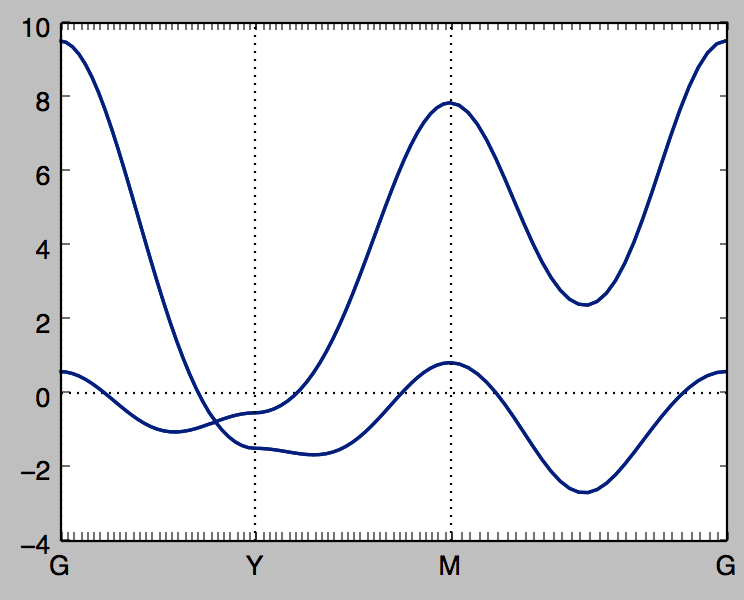
\includegraphics[scale=0.3]{./figs/fig01-14.png}
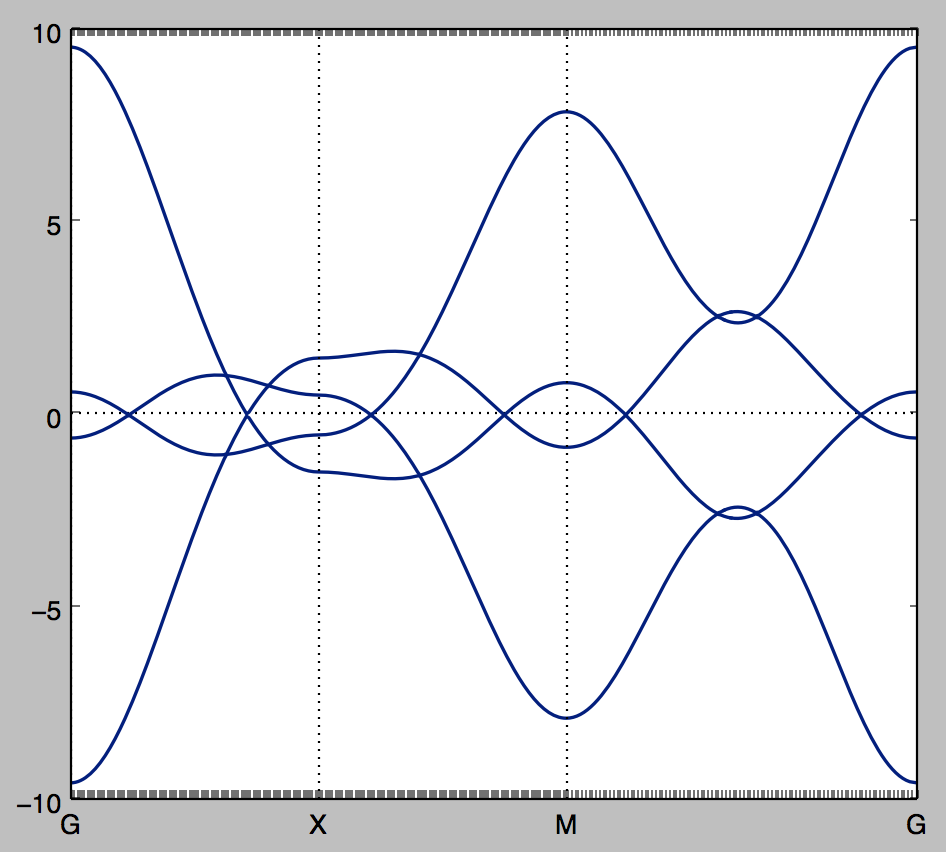
\includegraphics[scale=0.211]{./figs/fig01-15.png}
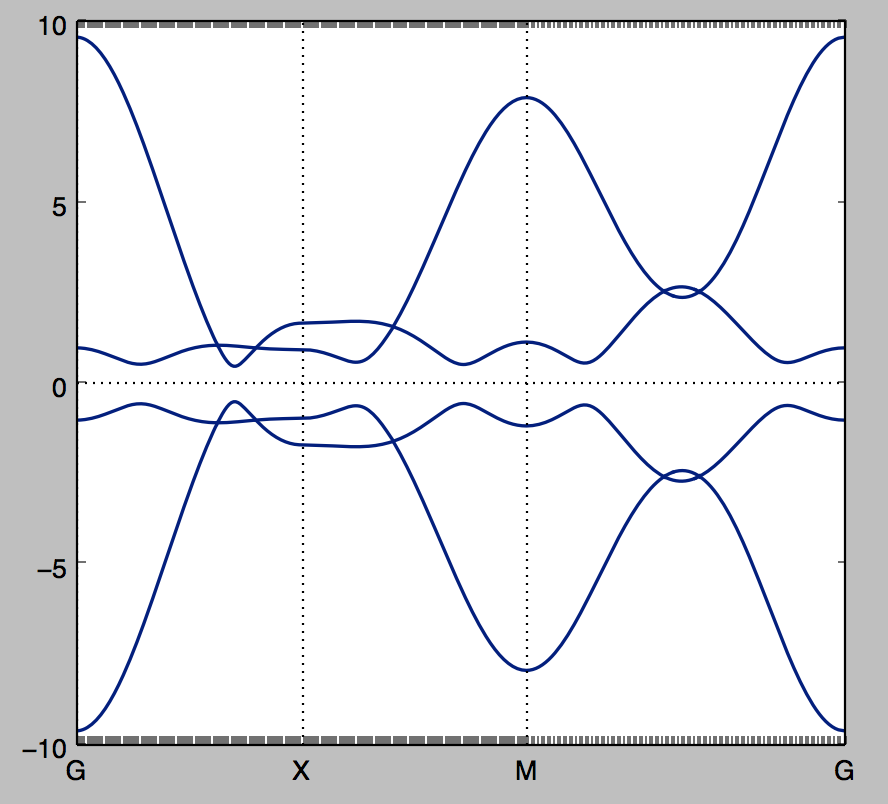
\includegraphics[scale=0.224]{./figs/fig01-16.png}
\caption{Band structure of the 2-orbital model of BaFe$_2$As$_2$ (left).
Band structure of the 2-orbital model of BaFe$_2$As$_2$ with [space = ``nambu"] option (middle).
S$\pm$ pairing superconducting band structure of the 2-orbital model of BaFe$_2$As$_2$ (right).}
\label{fig01-16}
\end{figure}


The calculated band structure is shown in Fig.~\ref{fig01-16} (left).
To construct the superconducting structure with TBM$^3$, we just have to change line 13 of ``BaFe2As2.lat.tbm" into,
\begin{lstlisting}[language=C++]
space = "nambu"
\end{lstlisting}
Therefore, the band structure will show particle-hole symmetry of spin-up and spin-down component, see Fig.~\ref{fig01-16} (middle).

Finally, we include the singlet next nearest neighbor S$\pm$ superconducting pairing symmetry to the model,
\begin{lstlisting}[language=C++]
pairingS  > Fe:Fe:+1+1+0 1:1 > -0.2
pairingS  > Fe:Fe:-1-1+0 1:1 > -0.2
pairingS  > Fe:Fe:+1-1+0 1:1 > -0.2
pairingS  > Fe:Fe:-1+1+0 1:1 > -0.2
pairingS  > Fe:Fe:+1+1+0 2:2 > -0.2
pairingS  > Fe:Fe:-1-1+0 2:2 > -0.2
pairingS  > Fe:Fe:+1-1+0 2:2 > -0.2
pairingS  > Fe:Fe:-1+1+0 2:2 > -0.2
\end{lstlisting}
, and the superconducting gap is presented, see Fig.~\ref{fig01-16} (right).
Note that, we can also perform a mean-field self-consistent iteration for the pairing orders by enable the ``isCalculateVar",
\begin{lstlisting}
isCalculateVar = 1
\end{lstlisting}
The value ``-0.2" here, is refered to the pairing potential and it should be ``attractive" to get effective pairings.
The BCS Hamiltonian is derived from the following equation,
\begin{equation}
H = \sum_{i\alpha\sigma j\beta\sigma'} h_{i\alpha\sigma,j\beta\sigma'} c^\dagger_{i\alpha\sigma} c_{j\beta\sigma'}
	+ \sum_{i\alpha j\beta} V_{ij} n_{i\alpha} n_{j\beta},
\end{equation}
and in this example $V_{ij} = -0.2$.
Please see more details in the {\bf TBM$^3$ Document} section.

\clearpage

\subsection{Setup the Wannier90 input file as the source of hopping terms} 
 This section demonstrate how TBM$^3$ calculation could be done with the tight binding Hamiltonian provided by  Wannier90\cite{W90-1,W90-2} calculation.  The Hamiltonian data could be written in terms of TBM$^3$ expressions through {\bf tbm-wannier}. The Wannier90 calculations of the following examples were based on the WIEN2k\cite{win} and wien2wannier-1.0\cite{W2W} calculations. 

% Full-potential linearized augmented plane wave density functional theory code (), maximally localized Wannier function method (Wannier90\cite{W90-1,W90-2}), and the interface between WIEN2k and Wannier90 () are employed.  


\subsubsection{Pb}
The face-centered cubic Pb ($a_0$=9.354144 a.u.) has well-defined six p orbitals around Fermi level.  
{\bf [filename]$\_$hr.dat} provided by Wannier90 calculation  has the below informations.
\begin{lstlisting}[language=C++]
 written on  9Jun2016 at 09:19:44 
 3
 3055    
  3    2    2    3    2    3    3    2  ...
  ...
-10    2    4    1    1   -0.000055    0.000000
-10    2    4    2    1   -0.000007   -0.000000
...   
0    0    0    1    1    1.488350   -0.000000
0    0    0    2    1   -0.000000    0.000000
0    0    0    3    1    0.000000   -0.000000
0    0    0    1    2   -0.000000   -0.000000
0    0    0    2    2    1.488350   -0.000000
0    0    0    3    2    0.000000   -0.000000
0    0    0    1    3    0.000000    0.000000
0    0    0    2    3    0.000000    0.000000
0    0    0    3    3    1.488350   -0.000000
...
 ...        
\end{lstlisting}
The first line is just a comment. The numbers in the second and third lines represent number of Wannier functions and number of the translation vector ($\delta$), respectively. There are 3 Wannier ($p_x$, $p_y$, $p_z$) functions and 3055 translation vectors.
From the 4th line to before starting of the hopping information, the degeneracies ($n_{\delta}$) of hopping terms for each translation vector ($\delta$) are addressed.
In the 7th line, -10, 2, and 4 means $\delta$=(-10,2,4) in terms of the primitive translation vector. Next two numbers of 2 and 1 are the orbital index ($\beta$, $\alpha$), respectively. The last two values are the real and imaginary part of the hopping term. 
The hopping Hamiltonian has the below form,
\begin{equation}
H = \sum_{ n_{\delta} \delta, \alpha\beta\, \sigma} \frac{t_{\alpha;\delta,\beta}}{n_{\delta}}\;\; c_{0+\delta, \alpha\sigma}^{\dagger} c_{0,\beta\sigma}.
\label{w90-eq}
\end{equation}

Using {\bf tbm-wannier}, {\bf [filename]$\_$.dat} could be converted into the input files for TBM$^3$.  {\bf tbm-wannier} needs the information about lattice({\bf\#BasisVector}), Wannier function({\bf\#AtomSetup}), and how many hopping terms are considered ({\bf\#Parameters}).  The example of the input file {\bf [filename].w90} is given below.
\begin{lstlisting}[language=C++]
#Parameters
spin    = "off"
bondN   =10,10,10
precision = 0.000001

#BasisVector
0.0000000   4.6770720   4.6770720
4.6770720   0.0000000   4.6770720
4.6770720   4.6770720   0.0000000

#AtomSetup
Pb > 0.000000000  0.000000000  0.000000000 > px py pz

#Wannier   
3    2    2    3    2    3    3    2  ...
...
-10    2    4    1    1   -0.000055    0.000000
-10    2    4    2    1   -0.000007   -0.000000
...   
0    0    0    1    1    1.488350   -0.000000
0    0    0    2    1   -0.000000    0.000000
0    0    0    3    1    0.000000   -0.000000
0    0    0    1    2   -0.000000   -0.000000
0    0    0    2    2    1.488350   -0.000000
0    0    0    3    2    0.000000   -0.000000
0    0    0    1    3    0.000000    0.000000
0    0    0    2    3    0.000000    0.000000
0    0    0    3    3    1.488350   -0.000000
...
...
\end{lstlisting}


\begin{itemize}
	\item {\bf\#Parameters} set spin-degeneracy ({\bf spin}) and how many hopping terms are included based on the hopping value ({\bf precision}) and translation vector({\bf bondN})\\
	\item {\bf\#BasisVector} setup the primitive translation vectors  $a_1$,$a_2$,$a_3$ (found in {\bf [filename].win}) The below $a_1$,$a_2$,$a_3$ are written in the Cartesian coordinate.\\
	\begin{align}
	a_1 &=(0.0000000,   4.6770720,   4.6770720 ) \nonumber\\
	a_2 &=(4.6770720,   0.0000000,   4.6770720 )\nonumber\\
	a_3 &=(4.6770720,   4.6770720,   0.0000000 )\nonumber
	\end{align}
	\item {\bf\#AtomSetup} setup atomic information and initial Wannier function(found in {\bf [filename].win}. The atomic coordinate needs to be written in  the Cartesian coordinate.\\
	\item {\bf\#Wannier} the same content to from fourth to last lines in {\bf [filename]$\_$hr.dat}\\
\end{itemize}.


By running "tbm-wannier" as shown below, you could have the TBM$^3$ input files ({\bf [filename].lat}, {\bf [filename].lat.tbm}).

\begin{lstlisting}[language=C++]
\$> tbm-wannier Pb.w90
Converting with ..
spin = off
bondN = [[ (10,0)      (10,0)      (10,0)     ]]
precision = 1e-06
\end{lstlisting}

\begin{itemize}
	\item {\bf[filename].lat} lattice  information\\
	\item {\bf[filename].lat.tbm} hopping Hamiltonian\\
\end{itemize}


The contents of {\bf [filename].lat.tbm} are shown below.

\begin{lstlisting}[language=C++]
#Parameters
TB_bond_alpha = 1.0 

#Hamiltonian
hopping  >  Pb-1:Pb-1:+28.0624-28.0624-37.4166           1:1      >  (-1.83333e-05,0) * TB_bond_alpha
hopping  >  Pb-1:Pb-1:+28.0624-28.0624-37.4166           2:1      >  (-2.33333e-06,-0) * TB_bond_alpha
...
hopping  >  Pb-1:Pb-1:+0+0+0                             1:1      >  (1.48835,-0)
hopping  >  Pb-1:Pb-1:+0+0+0                             2:2      >  (1.48835,-0)
hopping  >  Pb-1:Pb-1:+0+0+0                             3:3      >  (1.48835,-0)
...
\end{lstlisting}
the {\bf [filename].lat.tbm} script has three blocks to describe the model:
\begin{itemize}
	\item {\bf\#Parameters} {\bf TB$\_$bond$\_$alpha} is the renormalization factor for hopping term\\
	\item {\bf\#Hamiltonian} the converted hopping terms \\
\end{itemize}

Running {tbm-run} with the given  {\bf [filename].lat.tbm} and {\bf [filename].lat} will give nothing. The such input parameters   should be added, as shown in the following ({\bf control.tbm}).

\begin{lstlisting}[language=C++]
#Parameters
isCalculateMu   = 0 
isCalculateVar  = 0 
isCalculateBand = 1 
isCalculateLDOS = 0 

bandPoints      = 20

spin = "on"
space = "normal"
Nb          = 1,1,1
MF_diff    = 0.0001
MF_mix     = 0.2   

Mu          = 0

#KPointPath
G      0     0     0    
L      0     0.5   0    
K      0.38  0.75  0.38    
W      0.5   0.75  0.25 
X      0.5   0.50  0.   
G      0     0     0  
\end{lstlisting}


{\bf control.tbm} could be added into {\bf [filename].lat.tbm}, using {\bf Import} block.
\begin{lstlisting}[language=C++]
#Import 
"control.tbm"

#Parameters
TB_bond_alpha = 1.0 

#Hamiltonian
hopping  >  Pb-1:Pb-1:+28.0624-28.0624-37.4166           1:1      >  (-1.83333e-05,0) * TB_bond_alpha
hopping  >  Pb-1:Pb-1:+28.0624-28.0624-37.4166           2:1      >  (-2.33333e-06,-0) * TB_bond_alpha
...
hopping  >  Pb-1:Pb-1:+0+0+0                             1:1      >  (1.48835,-0)
hopping  >  Pb-1:Pb-1:+0+0+0                             2:2      >  (1.48835,-0)
hopping  >  Pb-1:Pb-1:+0+0+0                             3:3      >  (1.48835,-0)
...
\end{lstlisting}

\begin{itemize}
	\item {\bf\#Import} Load the prepared input parameters (added manually)\\
\end{itemize}

Pb-1 represents the first type of Pb atom in the material, 1:1 means the hopping first orbital (px) and first orbital (px), and +28.0624-28.0624-37.4166 shows the translation vector $\tau$ (+28.0624,-28.0624,-37.4166).
$\tau$ coulbe be explicitly written in terms of {\bf BasisVector},.
\begin{equation}
 \tau=-10*a_1 + 2*a_2+4*a_3    d
\end{equation}
The value of  $\frac{t_{p_x \uparrow \tau, p_x \uparrow}}{n_{\tau}}$ was computed by Eq \ref{w90-eq}, as shown below.
\begin{equation}
(-1.83333e-05,0)= (-0.000055/3,0)
\end{equation}
The removal of the hopping terms outside {\bf precision} and {\bf bondN} could be confirmed by a comparison of the hopping terms in between {\bf [filename].lat.tbm} and {\bf [filename].w90}.


\subsubsection{SrFeO$_3$}
The cubic SrFeO$_3$ ($a_0$=7.27735 a.u.) has well-defined five Fe d  and nine O p orbitals around Fermi level.
After the Wannierf90 calcuation, {\bf [filename]$\_$hr.dat}  has the below informations.


\begin{lstlisting}[language=C++]
 written on 28Apr2016 at 16:38:50 
 14
 125
 8    4    4    4    8    4    2    2    2    4    4    2    2    2    4
 4    2    2    2    4    8    4    4    4    8    4    2    2    2    4
 2    1    1    1    2    2    1    1    1    2    2    1    1    1    2
 4    2    2    2    4    4    2    2    2    4    2    1    1    1    2
 2    1    1    1    2    2    1    1    1    2    4    2    2    2    4
 4    2    2    2    4    2    1    1    1    2    2    1    1    1    2
 2    1    1    1    2    4    2    2    2    4    8    4    4    4    8
 4    2    2    2    4    4    2    2    2    4    4    2    2    2    4
 8    4    4    4    8
 -2   -2   -2    1    1   -0.000049   -0.000000
 -2   -2   -2    2    1   -0.000000   -0.000000
...
 -1   -1    0    7    1    0.032601   -0.000000
 -1   -1    0    8    1    0.026543    0.000000
...
...        
\end{lstlisting}
There are 14 Wannier functions with five d and nine p orbitals. 125 translation vectors are considered to generated hopping terms.

The example of the input file for {\bf tbm-wannier} is shown below.
\begin{lstlisting}[language=C++]
#Parameters
spin    = "off"
bondN   = 3, 3, 3
precision = 0.01

#BasisVector
7.2773350   0.0000000   0.0000000
0.0000000   7.2773350   0.0000000
0.0000000   0.0000000   7.2773350

#AtomSetup
Fe > 0.000000000  0.000000000  0.000000000 > dxy dxz dyz dx2-y2 dz2
O  > 3.638670000  0.000000000  0.000000000 > px py pz 
O  > 0.000000000  0.000000000  3.638670000 > px py pz 
O  > 0.000000000  3.638670000  0.000000000 > px py pz

#Wannier
8    4    4    4    8    4    2    2    2    4    4    2    2    2    4
4    2    2    2    4    8    4    4    4    8    4    2    2    2    4
2    1    1    1    2    2    1    1    1    2    2    1    1    1    2
4    2    2    2    4    4    2    2    2    4    2    1    1    1    2
2    1    1    1    2    2    1    1    1    2    4    2    2    2    4
4    2    2    2    4    2    1    1    1    2    2    1    1    1    2
2    1    1    1    2    4    2    2    2    4    8    4    4    4    8
4    2    2    2    4    4    2    2    2    4    4    2    2    2    4
8    4    4    4    8
-2   -2   -2    1    1   -0.000049   -0.000000
-2   -2   -2    2    1   -0.000000   -0.000000
...
-1   -1    0    7    1    0.032601   -0.000000
-1   -1    0    8    1    0.026543    0.000000
...
\end{lstlisting}
The translation vectors are given as below,
	\begin{align}
	a_1 &=(7.2773350,   0.0000000,   0.0000000 ) \nonumber\\
	a_2 &=(0.0000000,   7.2773350,   0.0000000 ) \nonumber \\
	a_3 &=(0.0000000,   0.0000000,   7.2773350 )  \nonumber
	\end{align}
The atomic coordinates for atoms are given below,
	\begin{align}
	r_{Fe-1} &=( 0.000000000  0.000000000  0.000000000) \nonumber \\
	r_{O-2} &=(3.638670000  0.000000000  0.000000000 ) \nonumber\\
    r_{O-3} &=(0.000000000  3.638670000  0.000000000 ) \nonumber\\
    r_{O-4} &=(0.000000000  0.000000000  3.638670000 )\nonumber
	\end{align}

After running {\bf tbm-wannier}, the generated {\bf [filename].lat} and {\bf [filename].lat.tbm} are shown below.
\begin{lstlisting}[language=C++]
#BasisVector
7.27733         0               0    
0               7.27733         0    
0               0               7.27733    

#OrbitalProfile
Fe-1        dxy dxz dyz dx2-y2 dz2 
O-2         px py pz
O-3         px py pz
O-4         px py pz

#Atoms
1           0.000000000  0.000000000  0.000000000 
2           3.638670000  0.000000000  0.000000000 
3           0.000000000  0.000000000  3.638670000 
4           0.000000000  3.638670000  0.000000000 
\end{lstlisting}
\begin{lstlisting}[language=C++]
#Parameters
TB_bond_alpha = 1.0 

#Hamiltonian
hopping  >  O-2:Fe-1:-10.916-7.27733+0                   2:1      >  (0.032601,-0) * TB_bond_alpha
hopping  >  O-2:Fe-1:-10.916-7.27733+0                   3:1      >  (0.026543,0) * TB_bond_alpha
...
\end{lstlisting}
The hopping terms outside {\bf precision} and {\bf bondN} were automatically removed in {\bf [filename].lat.tbm}. Fe and three O atoms are named as Fe-1, O-2, O-3, and O-4 in {\bf [filename.].lat}.  2:1 and 3:1 represent p$_y$(second orbital in O-2):d$_{xy}$(first orbital in Fe-1) and p$_z$(third orbital in O-2):d$_{xy}$, respectively. As O-2 and Fe-1 atoms have different atomic coordinates, the translation vector -10.916-7.27733+0 $\tau$ for hopping terms is given the below relation,
\begin{equation}
\tau=-1*a_1 -1*a_2+0*a_3 -r_{O-2}
\end{equation}





\subsection{Setup model parameters for spin-orbital coupling} 
How spin-orbital coupling manually could be implemented will be shown here. The spin-orbital coupling is expressed below. 
%\subsection{Identifying topological properties in using k-space dependent wannier center tecnique} 
%The content of this part will be filled later ...
\begin{align}
\lambda \vec{L} \cdot \vec{S} &= \lambda \lbrace  \frac{L_{+}S_{-} +L_{-} S_{+} }{2} +L_{z} S_{z} \rbrace 
\end{align}

$L_{\pm}$ and $S_{\pm}$ can be easily computed the below relation.
\begin{align}
L_{+} | l ,m \rangle &= \sqrt{l \cdot (l+1)-m \cdot (m+1)} |l, m+1 \rangle \\
L_{-} | l ,m \rangle &= \sqrt{l \cdot (l+1)-m \cdot (m-1)} |l,m-1 \rangle 
\end{align}

\begin{align}
S_{+} | \downarrow \rangle &=  |S_{z}= \uparrow \rangle \\
S_{-} | \uparrow  \rangle &=  |S_{z}= \downarrow \rangle 
\end{align}


As Pb has only $p$ electrons,  $|l=1,m,\sigma \rangle =| m \sigma\rangle$ is used. Using the below bases, the spin-orbit matrix (\ref{SO_matrix}) is constructed.  

\begin{equation}
|\rangle =| 1\uparrow, 1\downarrow, 0\uparrow, 0\downarrow, -1\uparrow, -1\downarrow \rangle
\end{equation}

\begin{align}
c1&= \sqrt{2}/2\\
\langle l m \sigma| \lambda \vec{L} \cdot \vec{S}|l'm' \sigma' \rangle 
&= \lambda
\left[ 
\begin{matrix}
0.5        & 0.         &0.      &   0.         &0.         &0.       \\ 
0.        & -0.5         &c1      &   0.         &0.         &0.       \\ 
0.        & c1         &0.     &   0.         &0.         &0.       \\ 
0.        & 0.         &0.      &  0.        & c1        &0.       \\ 
0.        & 0.         &0.      &   c1         &-0.5         &0.       \\ 
0.        & 0.         &0.      &   0.         &0.         &0.5       \\
\end{matrix}
\right] 
\label{SO_matrix}
\end{align}


As Wannier function ($\omega$) is different from the above state, \ref{SO_matrix} should be transformed into the matrix with  $\omega$.
\begin{align}
\langle \omega \sigma | \lambda \vec{L} \cdot \vec{S} | \omega \sigma  \rangle &= \sum_{l,m,l',m'}\langle \omega \sigma | lm \sigma \rangle  \langle
lm \sigma |\lambda \vec{L} \cdot \vec{S} | l'm' \sigma \rangle \langle l'm' \sigma | \omega \sigma \rangle  
\end{align}

The elements for $\langle lm  \sigma| \omega  \sigma \rangle $ could be found in {\bf  [filename].inwf}. As $\omega$ for $p$ electron is $p_x$, $p_y$,$p_z$, shown in \ref{p-wannier}, the new spin-orbit matrix (\ref{New_SO_matrix}) is derived.  
 
\begin{equation}
|\rangle =| px\uparrow, px\downarrow,  py\uparrow, py\downarrow,  pz\uparrow, pz\downarrow \rangle
\label{p-wannier}
\end{equation}

\begin{align}
\lambda
\left[ 
\begin{matrix}
0.        & 0.         &(0,0.5)      &   0.         &0.         &(0.5,0)       \\ 
0.        & 0.         &0.      &  (0,-0.5)         & (-0.5,0)        &0.       \\ 
(0,-0.5)        & 0.         &0.      &   0.         &0.         &(0,0.5)       \\ 
0.        & (0,0.5)         &0.      &   0.         &(0,0.5)         &0.       \\ 
0.        & (-0.5,0)         &0.      &   (0,-0.5)         &0.         &0.       \\ 
(0.5,0)        & 0.         &(0,-0.5)      &   0.         &0.         &0.       \\
\end{matrix}
\right] 
\label{New_SO_matrix}
\end{align}

Using \ref{New_SO_matrix}, the spin-orbit term could be implemented as below. The strength could be controlled by the parameter {\bf so}, which corresponds to $\lambda$ in the above formula.
\begin{lstlisting}[language=C++]
#Hamiltonian
site>Pb-1 px.u:py.u > (0.0,0.5)*so  
site>Pb-1 px.u:pz.d > (0.5,0.0)*so  
site>Pb-1 px.d:py.d > (0.0,-0.5)*so  
site>Pb-1 px.d:pz.u > (-0.5,0.0)*so  
site>Pb-1 py.u:px.u > (0.0,-0.5)*so  
site>Pb-1 py.u:pz.d > (0.0,0.5)*so  
site>Pb-1 py.d:px.d > (0.0,0.5)*so  
site>Pb-1 py.d:pz.u > (0.0,0.5)*so  
site>Pb-1 pz.u:px.d > (-0.5,0.0)*so  
site>Pb-1 pz.u:py.d > (0.0,-0.5)*so  
site>Pb-1 pz.d:px.u > (0.5,0.0)*so  
site>Pb-1 pz.d:py.u > (0.0,-0.5)*so 
\end{lstlisting}




\clearpage
\subsection{Identifying $Z_2$ Topological Index in using the Wannier center tecnique}
To calculate the $Z_2$ topological invariant of band insulators, 
we utilize the methodology of winding number of Wilson loop operator defined by non-Abelian Berry connection \cite{XDai2011,Vanderbilt2011}.
The current strategy, derived from evolution of Wannier function centers during time-reversal pumping \cite{XLQi2011}, is
equivalent to the $Z_2$ topological invariant proposed by Kane and Mele \cite{Kane05}.
The advantage of current method is one can identify the topological nature of a general band insulator without any of the
gauge-fixing problems or additional requirement of inversion symmetry.
Now we briefly explain the formula related to the method.

Supposed that we have $2N$ occupied bands,
a $U(2N)$ Berry phase gauge field is defined as $a_{i}^{nm}=-i\langle nk|\partial_{i}|mk\rangle$,
where $|mk\rangle$ is the Bloch wavefunction of the $m-$th band.
Then we can define the $U(2N)$ Wilson loop along the same
equal-$k_{y}$ loops:

\begin{eqnarray}
W(k_{y})=Pe^{i\oint dk_{x}a_{x}(k_{x},k_{y})}\in U(2N)
\end{eqnarray}
, and the $U(1)$ flux $\Phi(k_{y})$
related to $W(k_{y})$ is defined as $e^{i\Phi(k_{y})}=\det W(k_{y})$. Denote
the eigenvalues of $W(k_{y})$ as $e^{i\phi_{n}(k_{y})}$ with $n=1,..,2N$,
we have $\Phi(k_{y})=\sum_{n}\phi_{n}(k_{y})~{\rm ~mod~}2\pi$. Thus,
the $Z_2$ invariant can be expressed as

\begin{equation}
\begin{aligned}
\label{eq:z2forU2N}
\Delta =\frac{1}{2\pi}\Big(&\sum_{n}\int_{0}^{\pi}dk_{y}\partial_{k_{y}}\phi_{n}(k_{y})
		-\sum_{n}\left(\phi_{n}(\pi)-\phi_{n}(0)\right)\Big) {\rm ~mod~}2
\end{aligned}
\end{equation}

To simplify the formula, we choose $\phi_{n}(0)$ and $\phi_{n}(\pi)$ to be in $[0,2\pi)$:

\begin{eqnarray}
\int_{0}^{\pi}dk_{y}\partial_{k_{y}}\phi_{n}(k_{y})=\phi_{n}(\pi)-\phi_{n}(0)+2\pi M_{n}
\end{eqnarray}

 with $M_{n}$ the winding number of phase $\phi_{n}$, which is equal
to the number of times $\phi_{n}$ crosses the line $\phi_{n}=2\pi$
from below.  In this
way we get

\begin{eqnarray}
\Delta=\sum_{n}M_{n}~{\rm ~mod~}2
\end{eqnarray}

The number $\sum_{n}M_{n}$ simply counts how many eigenvalues $\phi_{n}$
crosses $\phi=2\pi$ line (or any other reference line).
Thus the $Z_{2}$ invariant is simply determined by the parity of
the number of eigenvalue curves $\phi_{n}(k_{y})$ which crosses a
reference line $\phi={\rm constant}$.

At last, we have several remarks here.
First, the current methodology are relevant to the theory of maximally localized Wannier functions.
In one dimension, Berry phases represent spatial coordinates of the maximally localized Wannier functions.
In higher dimensions, these phases are the spatial coordinates of hybrid Wannier functions, which maximally localize along one direction (saying $\hat x$), but extend in the remaining directions as a Bloch wave.
The derivative of the geometric Berry phase, is interpreted as the real-space velocity (in $\hat x$ direction) of the m'th Wannier center.
By integrating the velocities of all Wannier centers on other directions over a period, we obtain the net quantum (spin) Hall current, directly relating to topological Chern number ($Z_2$ number) \cite{XLQi2011}.
Second, the current method is based on tracking the evolution of Wannier center, which is equivalent to the computation of the winding number of Wilson loop operator. 
Thus, the current method is not only limited to calculating $Z_2$ invariants of time-reversal invariant topological insulator, but also capable of calculating Chern number in time-reversal breaking topological states. 
Moreover, through the use of individual Chern numbers it can be used to identify any kind of topological phases, such as topological crystalline insulators.

We have employed this techique in TBM$^3$ package, and it can be simply applied with the {\bf \#KWannierPath} block.
However, this function is still under testing and we will soon update this document to describe it in more details.


\cleardoublepage

\section{TBM$^3$ Document}
The programming flow of TBM$^3$ can be generally described in the following figure.
In this flow chart, we show an auxiliary matrix (with spin=``on" and space=``normal") is created to calculate the chemical potential in using the binary search alogrithm.
In the case of superconductivity calculations, the binary search algorithm cannot be applied to the BdG matrix; therefore, the auxiliary matrix helps boost the iteration progress in compare to other method that finding chemical potential with the BdG matrix in linear time.

In most cases, the bottleneck of the calculation efficiency depends on the diagonalization efficiency, and we can pass this task to GPU to accelerate the speed.
However, it may not be necessary to use the GPU scheme for all of the cases.
We suggest to use the GPU calculations when the real-space lattice is large.
Please see {\bf subsection I.} to change the matrix solver.

\begin{center}
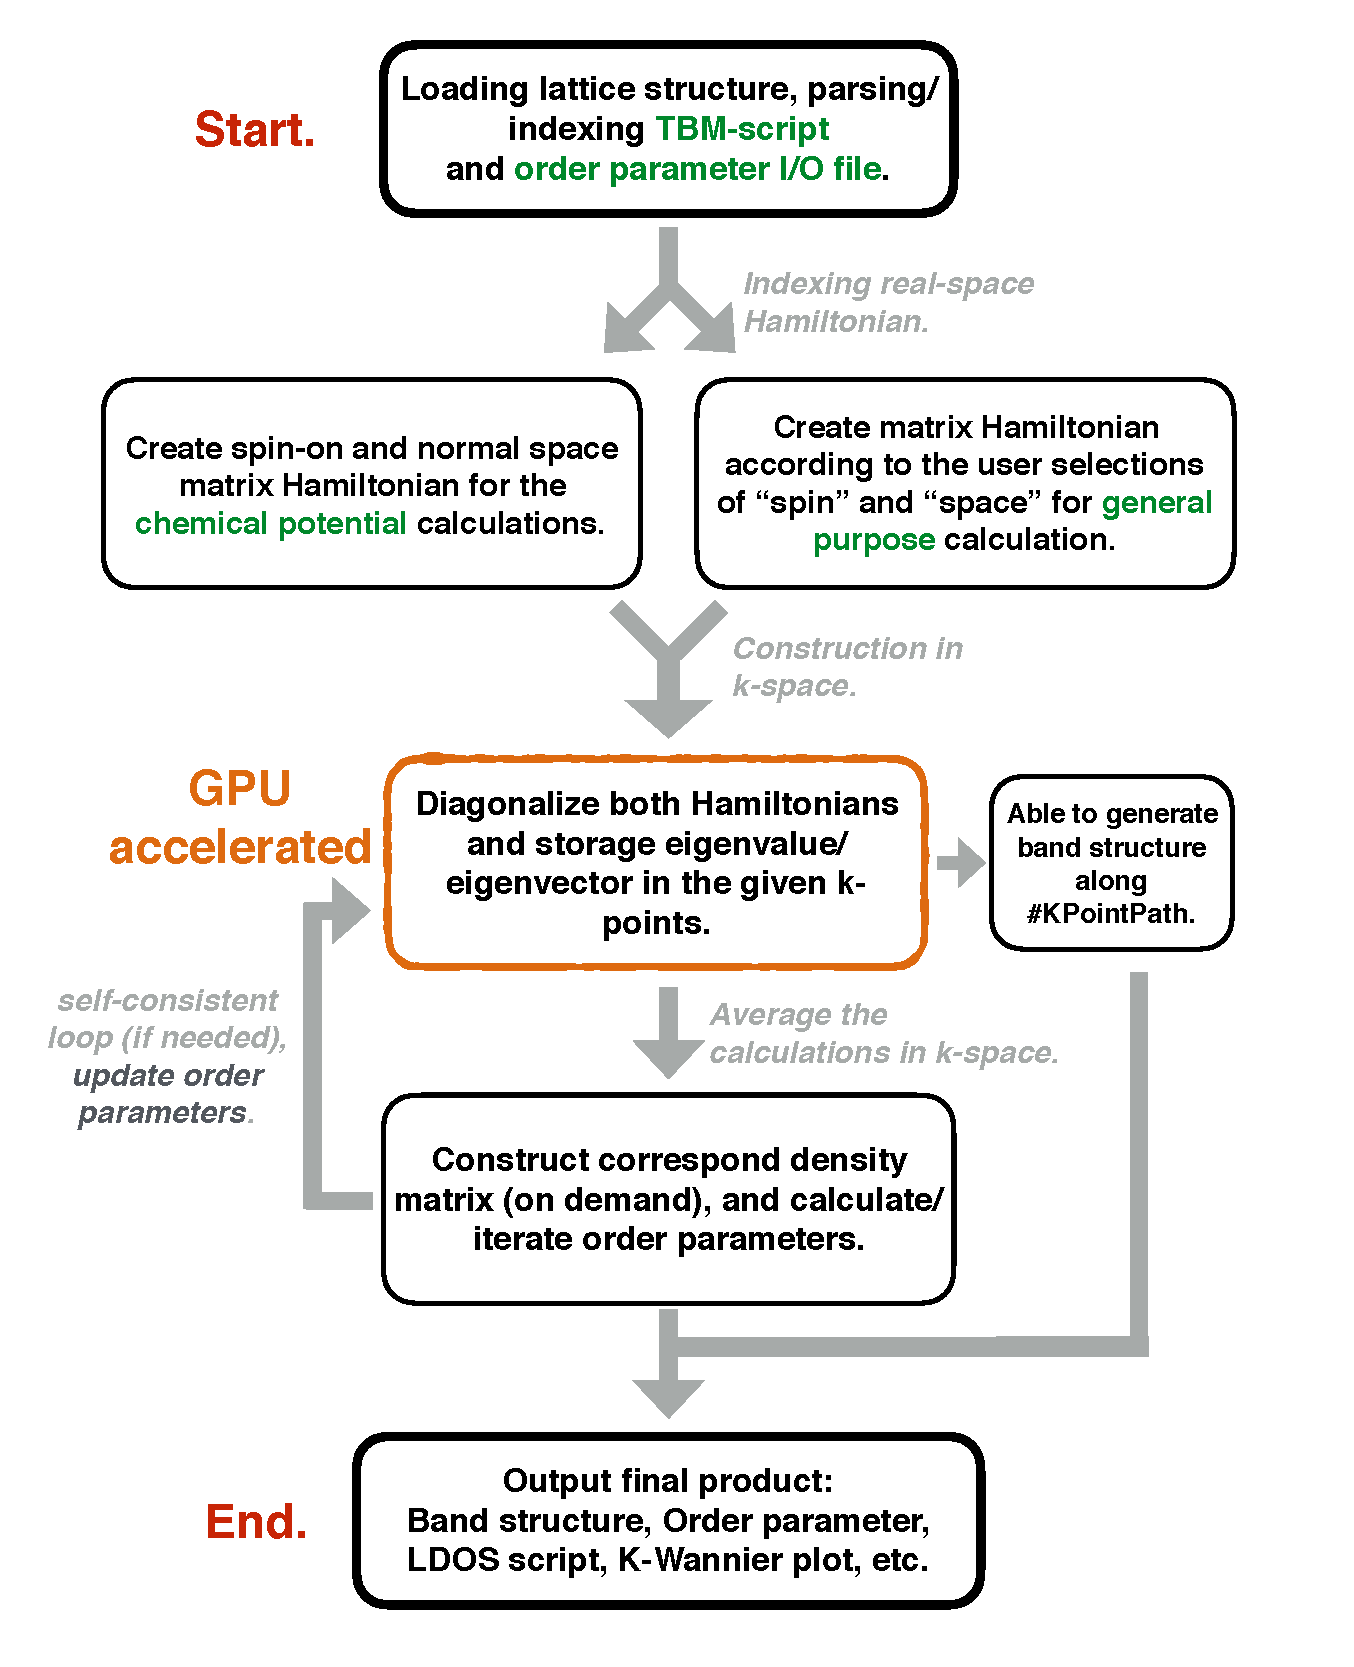
\includegraphics[scale=0.6]{./TBMCube-flow}
\end{center}

\clearpage


\subsection{The ``Blocks" notation of lattice \& TBM-script input file} 
The body of all of the input files are defined by the ``Blocks" notation following by the ``\#" symbol.
The following blocks are used in the lattice input file, {\bf [file-name].lat},
\begin{lstlisting}[language=C++]
#BasisVector
...
#OrbitalProfile
...
#Atoms
...
\end{lstlisting}
These three blocks {\bf\#BasisVectore}, {\bf\#OrbitalProfile} and {\bf\#Atoms} are required in the lattice input file ``*.lat".
On the other hand, the following blocks for the TBM-script, ``*.lat.tbm", are conditionally required.
\begin{lstlisting}[language=C++]
#Import
...
#KPointPath
...
#BondVector [N=0,1,2,...]
...
#Parameters
...
#LDOSList
...
#Init
...
#Hamiltonian
...
\end{lstlisting}
Note that, in order to execute the task, TBM$^3$ requires at least two input files (*.lat and *.lat.tbm) to be prepared by the user.
Therefore, once we enter the following in ther terminal:


\begin{lstlisting}[language=C++]
\$> tbm-run [file-name].lat
\end{lstlisting}
TBM$^3$ will automatically looking for {\bf [file-name].lat.tbm}.
If the correspond ``tbm" file cannot be found, TBM$^3$ will print out an error message.

\begin{lstlisting}[language=C++]
\$> tbm-run [file-name].lat
Error: from [file-name].lat
 Cannot find import file: [file-name].lat.tbm
\end{lstlisting}


\subsection{Lattice input file structure} 

The first block for the lattice input file is {\bf \#BasisVector}:
\begin{lstlisting}[language=C++]
#BasisVector
1    0    0
0    1    0
0    0    1
\end{lstlisting}
The above described the a cubic cell.
Once we set this up, TBM$^3$ will use it to generate the periodic boundary condition and matching pairwised operation automatically. TBM$^3$ will also use the {\bf \#BasisVector} to calculate it's corresponding Bravis-vector ($b_1$, $b_2$, $b_3$) and generate its corresponding k-space phase for several calculations.

The next one is the {\bf \#OrbitalProfile} that describes the orbital content of each atom:
\begin{lstlisting}[language=C++]
#OrbitalProfile
Atom-Name1    s
Atom-Name2    px py pz
Atom-Name3    dxz dyz ...
...
\end{lstlisting}
When atoms are created, the {\bf tbm-run} program will associate the correspond atom names with its orbitals via the {\bf \#OrbitalProfile}. The above shows three different atoms, [Atom-Name1~2] that associated with different orbitals.
In principal, the `Atom-Name' could be arbitrary, however, the following characters are not allowed to use to build the `Atom-Name': `\%', `:', `\#' and  `$>$'.
These characters have special useage in the TBM-script.

On the other hand, the name of the orbitals are strictly bind to the following strings:
\begin{itemize}
\item s-orbital: s,
\item p-orbitals: px,  py,  pz,
\item d-orbitals: dxy,  dxz,  dyz,  dx2-y2,  dz2,
\item f-orbitals: fxz2,  fyz2,  fz3, fx(x2-3y2), fy(3x2-y2), fz(x2-y2), fxyz.
\end{itemize}

\subsection{The \#Import block of the TBM-script} 
The ``[filename].lat.tbm" file can be involved with many different blocks.
However, in many cases, the entire *.lat.tbm file may not keep its simplicity as for a simple model.
Therefore, the ``\#Import" block is to help to separate different parts of the *.lat.tbm file into different pieces of files.

To use it, we declare the following statement inside the ``*.lat.tbm" file:
\begin{lstlisting}[language=C++]
#Import
"anotherFile.tbm"
\end{lstlisting}
If one use the {\bf \#Import} block wisely, (s)he can increase the efficiency of the work flow.

Here we give an example of tutorial ``{\bf A}" that we can split the square.lat.tbm into two parts.
The first part contain the {\bf \#KPointPath}, {\bf \#Parameters} and {\bf \#CoreCharge} blocks with an additional {\bf \#Import} block:
\begin{lstlisting}[language=C++]
#KPointPath
G      0     0     0    
X      0.5   0     0    
M      0.5   0.5   0    
G      0     0     0    

#Parameters
isCalculateMu   = 1
isCalculateBand = 1
Nb = 4,4,1

spin = "on"
space = "normal"
bondRadius = 1

t  =  -1

#CoreCharge
Cu  >  1

#Import
"hamiltonian.tbm"
\end{lstlisting}
and the second part, ``hamiltonian.tbm", contain the {\bf \#Hamiltonian} block: 
\begin{lstlisting}[language=C++]
% The "hamiltonian.tbm" file
#Hamiltonian
hopping  >  Cu:Cu:+1+0+0  1:1  > t
hopping  >  Cu:Cu:-1+0+0  1:1  > t
hopping  >  Cu:Cu:+0+1+0  1:1  > t
hopping  >  Cu:Cu:+0-1+0  1:1  > t
\end{lstlisting}



\clearpage
\subsection{The \#Hamiltonian block} 
The most important feature of TBM$^3$ is in using the simple script-type notation to describe each real-space interaction term of the Hamiltonian.
In following, we listed the terms which can be used in the {\bf \#Hamiltonian} block:

\begin{center}
\begin{tabular}{ | l | l | l | }
\hline
\;\;\makecell{\\{\bf Description}\\ \\}\;\; &  \;\;\makecell{\\{\bf TBM-script}\\ \\}\;\; & \;\;\makecell{\\{\bf Details}\\ \\}\;\;\\
\hline
	\makecell[l]{
	On-site orbital energy:\\
	\;\;$ v \sum_{i=X} c_{i, \alpha}^\dagger \, c_{i, \alpha}$\;\;
	}
	&
	\;\;orbital $>$ X \;\;$\alpha$ $>$ var \;\;
	&
	\;\;\makecell[l]{
		\\
    	X = atom name,\\
		$\alpha$ = orbital number,\\
		$v$ = var $\in$ real.  \\
		\\
	}\;\;
	\\
\hline
	\makecell[l]{
	\\
	Spin-dependent site coupling:\\
    \;\;$ v \sum_{i=X} c_{i, \alpha,\sigma}^\dagger \, c_{i, \beta, \sigma'} $\;\;
	\\
	\\
	Spin-dependent site coupling with H.C.:\\
    \;\;$ \sum_{i=X}( v\; c_{i, \alpha,\sigma}^\dagger \, c_{i, \beta, \sigma'} $ + $v^*\; c_{i, \beta,\sigma'}^\dagger \, c_{i, \alpha, \sigma})$\;\;\\
	\\
	}
	&
	\makecell[l]{
	\;\;site $>$ X \;\;$\alpha\sigma$:$\beta\sigma'$ $>$ var \;\;\\
	\\
	\;\;siteHc $>$ $X$ \;\;$\alpha\sigma$:$\beta\sigma'$ $>$ var\;\;
	}
	&
	\;\;\makecell[l]{
		\\
		X = atom name,\\
		$\alpha,\beta$ = orbital number,\\
		$\sigma,\sigma'$ = ``u",``d" $\in$ $\uparrow, \downarrow$,\\
		$v$=var $\in$ complex.\\
		\\
	}\;\;
	\\
\hline
	\;\;\makecell[l]{
	\\
	Hopping term:\\
	$ t\;\sum_{i=X, j=Y}\; c_{i\alpha}^\dagger \, c_{j\beta} $\\
	\\
	Hopping term with H.C.:\\
    $ \sum_{i=X, j=Y} (t\;c_{i\alpha}^\dagger \, c_{j\beta} + t^*\; c_{j\beta}^\dagger \, c_{i\alpha} ) $\\
	\\
	Spin-dependent bonding:\\
	$ t\;\sum_{i=X, j=Y}\; c_{i\alpha\sigma}^\dagger \, c_{j\beta\sigma'} $\\
	\\
	Spin-dependent bonding with H.C.:\\
    $ \sum_{i=X, j=Y} (t\;c_{i\alpha\sigma}^\dagger \, c_{j\beta\sigma'}+t^*\; c_{j\beta\sigma'}^\dagger \, c_{i\alpha\sigma} ) $\\
	\\
	($j=i+\delta$)
	}
	&
	\makecell[l]{
	\\
	\;\;hopping \;\;\;\,\,$>$ $X$:$Y$:+a+b+c\;\;$\alpha$:$\beta$\; $>$ var\;\;\\
	\;\;hopping \;\;\;\,\,$>$ $X$:$Y$:+a+b+c\#\;\;$\alpha$:$\beta$\; $>$ var\;\;\\
	\;\;hopping \;\;\;\,\,$>$ $X$:$Y$:+a+b+c\#n\;\;$\alpha$:$\beta$\; $>$ var\;\;\\
	\\
	\;\;hoppingHc $>$ $X$:$Y$:+a+b+c\;\;$\alpha$:$\beta$\; $>$ var\;\;\\
	\;\;hoppingHc $>$ $X$:$Y$:+a+b+c\#\;\;$\alpha$:$\beta$\; $>$ var\;\;\\
	\;\;hoppingHc $>$ $X$:$Y$:+a+b+c\#n\;\;$\alpha$:$\beta$\; $>$ var\;\;\\
	\\
	\;\;bond \;\;\;\,\,$>$ $X$:$Y$:+a+b+c\;\;$\alpha\sigma$:$\beta\sigma'$\; $>$ var\;\;\\
	\;\;bond \;\;\;\,\,$>$ $X$:$Y$:+a+b+c\#\;\;$\alpha\sigma$:$\beta\sigma'$\; $>$ var\;\;\\
	\;\;bond \;\;\;\,\,$>$ $X$:$Y$:+a+b+c\#n\;\;$\alpha\sigma$:$\beta\sigma'$\; $>$ var\;\;\\
	\\
	\;\;bondHc $>$ $X$:$Y$:+a+b+c\;\;$\alpha\sigma$:$\beta\sigma'$\; $>$ var\;\;\\
	\;\;bondHc $>$ $X$:$Y$:+a+b+c\#\;\;$\alpha\sigma$:$\beta\sigma'$\; $>$ var\;\;\\
	\;\;bondHc $>$ $X$:$Y$:+a+b+c\#n\;\;$\alpha\sigma$:$\beta\sigma'$\; $>$ var\;\;\\
	\\
	}
	&
	\;\;\makecell[l]{
	\\
	X,Y = atom name,\\
	$\alpha,\beta$ = orbital number,\\
	$t = $var $\in$ complex,\\
	$\delta = $ +a+b+c(\#n) $=$ bond direction,\\
	$n$ = 0, 1, 2, ... \\
	\;\;\;(indicate \#BondVector 0, 1, 2 ... )\\
	\\
	}\;\;
	\\
\hline
	\makecell[l]{
	\\
	Screened long-range Coulomb interaction:\\
    $\sum_{i=X, |\delta|\le R} \frac{\alpha * (n_i - Z_i) ( n_{j} - Z_{j})}{ |\delta|}\times e^{-|\delta|/R}$\\
	\\
	($j=i+\delta$)\\
	\\
	}
	&
	\;\;screenCoulomb $>$ $X$\;\; $\sim$$R$ $>$ @:den * var\;\;
	&
	\;\;\makecell[l]{
	\\
	X = atom name,\\
	$\sim$$R$ = cut-off radius,\\
	@:den $=$ $n_i$ = electron occupancy,\\
	$Z_i$ = core charge (ionic charge),\\
	$\alpha$ = var = Coulomb strength.\\
	\\
	}\;\;
	\\
\hline
	\makecell[l]{
	\\
	On-site Hubbard interaction (intra-orbital):\\
    $U \sum_{i} n_{i\alpha\uparrow} n_{i\alpha\downarrow}$\\
	\\
	On-site Dudarev interaction (intra-orbital):\\
    $\frac{(U-J)}{2} \sum_{i,\sigma} (n_{i\alpha\sigma} - n_{i\alpha\sigma}^2)$\\
	\\
	}
	&
	\makecell[l]{
	\\
	\;\;intraHubbard $>$ $X$ \;\;$\alpha$ $>$ varU\\
	\\
	\;\;intraDudarevUJ $>$ X \;\;$\alpha$ $>$ varUJ\\
	\\
	}
	&
	\;\;\makecell[l]{
	\\
	X = atom name, \\
	$\alpha$ = orbital, \\
	$U$ = varU,\\
	$(U-J)$ = varUJ.\\
	\\
	}\;\;
	\\
\hline
\end{tabular}
\end{center}
\begin{center}
\begin{tabular}{ | l | l | l | }
\hline
	\makecell[l]{
	\\
	External magnetic field to classical spin:\\
    $ \sum_{i=X} \vec B \cdot \vec S_{i} $\\
	\\
	External magnetic field to itinerant electron:\\
    $ \sum_{i=X,\sigma\sigma'} c^\dagger_{i\alpha\sigma}c_{i\alpha\sigma'} \vec B \cdot \vec \sigma_{i,\alpha} $\\
	\\
	}
	&
	\;\;\makecell[l]{
	\;\;fieldB $>$ $X$ $>$ [x,y,z] * var\;\;\\
	\\
	\;\;fieldB $>$ $X$ \;\;$\alpha$ $>$ [x,y,z] * var\;\;\\
	\\
	}
	&
	\;\;\makecell[l]{
	\\
    X = atom name,\\
    $\alpha$ = orbital number.\\
    $|B|$ = var $\in$ real,\\
	$\hat B$ = [x,y,z] = Unit vector,\\
	\\
	}\;\;
	\\
\hline
	\;\;\makecell[l]{
	\\
	Hund coupling:\\
	$ J_h \sum_{i=X, \sigma\sigma'} c_{i, \alpha,\sigma}^\dagger \, c_{i, \alpha, \sigma'} \vec S_i \cdot \vec\sigma_{i,\alpha} $\\
	\\
	}
	&
	\;\;hundSpin $>$ $X$ \;\;$\alpha$ $>$ @:cspin * var
	&
	\;\;\makecell[l]{
	\\
    X = atom name,\\
    $\alpha$ = orbital number,\\
    @:cspin $=$ $S_i$\\
	\;\;\;= site classical spin ($|S|=1$),\\
    $J_h$=var $\in$ real\\
	\\
	}\;\;
	\\
\hline
	\;\;\makecell[l]{
	\\
	Super exchange:\\
    $ J_{se} \sum_{i=X, j= Y} \vec S_i \cdot \vec S_{j} $\\
	\\
	DM exchange:\\
    $ J_{dm} \sum_{i=X, j= Y}\vec D(\delta)\cdot \vec S_i \times \vec S_{j} $\\
	\\
	($j=i+\delta$)\\
	}
	&
	\makecell[l]{
	\;\;superEx $>$ $X$:$Y$:+a+b+c $>$ @:cspin * var\;\;\\
	\;\;superEx $>$ $X$:$Y$:+a+b+c\# $>$ @:cspin * var\;\;\\
	\;\;superEx $>$ $X$:$Y$:+a+b+c\#n $>$ @:cspin * var\;\;\\
	\\
	\;\;dmEx $>$ $X$:$Y$:+a+b+c $>$ @:cspin * var\;\;\\
	\;\;dmEx $>$ $X$:$Y$:+a+b+c\# $>$ @:cspin * var\;\;\\
	\;\;dmEx $>$ $X$:$Y$:+a+b+c\#n $>$ @:cspin * var\;\;\\
	}
	&
	\;\;\makecell[l]{
	\\
    X,Y = atom name,\\
    @:cspin $=$ $S_i(S_j)$\\
	\;\;= site classical spin ($|S|=1$),\\
    $J_{se}$=var $\in$ real\\
    $J_{dm}$=var $\in$ real\\
	\\
	Note: $\vec D(\delta) = \hat\delta$\\
	\\
	$\delta = $ +a+b+c(\#n) $=$ bond direction,\\
	$n$ = 0, 1, 2, ... \\
	\;\;\;(indicate \#BondVector 0, 1, 2 ... )\\
	\\
	}\;\;
	\\
\hline
	\;\;\makecell[l]{
	\\
	On-site singlet pairing interaction:\\
	$ \sum_{i=X} (\Delta^s_{i\alpha\uparrow,i\beta\downarrow}\, c^\dagger_{i\alpha\uparrow} c^\dagger_{i\beta\downarrow}+h.c.)$\\ \\
	$\Delta^s_{i\alpha\uparrow,i\beta\downarrow}\equiv V_{i\alpha,i\beta}(\langle c_{i\alpha\uparrow}c_{i\beta\downarrow} - c_{i\alpha\downarrow}c_{i\beta\uparrow}\rangle)/2$\\
	\\
	On-site triplet pairing interaction for $\Delta_{\uparrow\downarrow}$:\\
	$ \sum_{i=X} (\Delta^t_{i\alpha\uparrow,i\beta\downarrow}\, c^\dagger_{i\alpha\uparrow} c^\dagger_{i\beta\downarrow}+h.c.)$\\ \\
	$\Delta^t_{i\alpha\uparrow,i\beta\downarrow}\equiv V_{i\alpha,i\beta}(\langle c_{i\alpha\uparrow}c_{i\beta\downarrow} + c_{i\alpha\downarrow}c_{i\beta\uparrow}\rangle)/2$\\
	\\
	On-site triplet pairing interaction for $\Delta_{\uparrow\uparrow}$:\\
	$ \sum_{i=X} (\Delta^t_{i\alpha\uparrow,i\beta\uparrow}\, c^\dagger_{i\alpha\uparrow} c^\dagger_{i\beta\uparrow}+h.c.)$\\ \\
	$\Delta^t_{i\alpha\uparrow,i\beta\uparrow}\equiv V_{i\alpha,i\beta}\langle c_{i\alpha\uparrow}c_{i\beta\uparrow}\rangle$\\
	\\
	On-site triplet pairing interaction for $\Delta_{\downarrow\downarrow}$:\\
	$ \sum_{i=X} (\Delta^t_{i\alpha\downarrow,i\beta\downarrow}\, c^\dagger_{i\alpha\downarrow} c^\dagger_{i\beta\downarrow}+h.c.)$\\ \\
	$\Delta^t_{i\alpha\downarrow,i\beta\downarrow}\equiv V_{i\alpha,i\beta}\langle c_{i\alpha\downarrow}c_{i\beta\downarrow}\rangle$\\
	\\
	}\;\;
	&
	\;\;\makecell[l]{
	pairingS $>$ \;\;$X$ \;\;$\alpha$:$\beta$ $>$ var\\ \\ \\
	\\
	pairingUD $>$ \;\;$X$ \;\;$\alpha$:$\beta$ $>$ var\\ \\ \\
	\\
	pairingUU $>$ \;\;$X$ \;\;$\alpha$:$\beta$ $>$ var\\ 
	($\alpha \neq \beta$)\\ \\
	\\
	pairingDD $>$ \;\;$X$ \;\;$\alpha$:$\beta$ $>$ var\\ 
	($\alpha \neq \beta$)\\ \\
	}\;\;
	&
	\;\;\makecell[l]{
		\\
    	X = atom name,\\
		$\alpha,\beta$ = orbital number,\\
		$V_{i\alpha,i\beta}$ = var $\in$ real.\\ \\
		Note: The order $\Delta_{i\alpha\sigma,i\beta\sigma'}$\\
		can be assigned in *.lat.ord\\
		as initial value.\\
		If not assigned, it will be\\
		given by a default value in\\ $\langle c_{i\alpha\sigma} c_{i\beta\sigma'}\rangle$.\\
		\\
	}\;\;
	\\
\hline
\end{tabular}
\end{center}
\begin{center}
\begin{tabular}{ | l | l | l | }
\hline
	\;\;\makecell[l]{
	\\
	Off-site singlet pairing interaction:\\
	$ \sum_{i=X,j=Y} (\Delta^s_{i\alpha\uparrow,j\beta\downarrow}\, c^\dagger_{i\alpha\uparrow} c^\dagger_{j\beta\downarrow}+h.c.)$\\ \\
	$\Delta^s_{i\alpha\uparrow,j\beta\downarrow}\equiv V_{i\alpha,j\beta}(\langle c_{i\alpha\uparrow}c_{j\beta\downarrow} - c_{i\alpha\downarrow}c_{j\beta\uparrow}\rangle)/2$\\
	\\
	Off-site triplet pairing interaction for $\Delta_{\uparrow\downarrow}$:\\
	$ \sum_{i=X,j=Y} (\Delta^t_{i\alpha\uparrow,j\beta\downarrow}\, c^\dagger_{i\alpha\uparrow} c^\dagger_{j\beta\downarrow}+h.c.)$\\ \\
	$\Delta^t_{i\alpha\uparrow,j\beta\downarrow}\equiv V_{i\alpha,j\beta}(\langle c_{i\alpha\uparrow}c_{j\beta\downarrow} + c_{i\alpha\downarrow}c_{j\beta\uparrow}\rangle)/2$\\
	\\
	Off-site triplet pairing interaction for $\Delta_{\uparrow\uparrow}$:\\
	$ \sum_{i=X,j=Y} (\Delta^t_{i\alpha\uparrow,j\beta\uparrow}\, c^\dagger_{i\alpha\uparrow} c^\dagger_{i\beta\uparrow}+h.c.)$\\ \\
	$\Delta^t_{i\alpha\uparrow,j\beta\uparrow}\equiv V_{i\alpha,j\beta}\langle c_{i\alpha\uparrow}c_{j\beta\uparrow}\rangle$\\
	\\
	Off-site triplet pairing interaction for $\Delta_{\downarrow\downarrow}$:\\
	$ \sum_{i=X,j=Y} (\Delta^t_{i\alpha\downarrow,j\beta\downarrow}\, c^\dagger_{i\alpha\downarrow} c^\dagger_{j\beta\downarrow}+h.c.)$\\ \\
	$\Delta^t_{i\alpha\downarrow,j\beta\downarrow}\equiv V_{i\alpha,j\beta}\langle c_{i\alpha\downarrow}c_{j\beta\downarrow}\rangle$\\
	\\
	$(j=i+\delta)$
	}\;\;
	&
	\;\;\makecell[l]{
	pairingS  $>$ \;\;$X$:$Y$:+a+b+c(\#) \;\;$\alpha$:$\beta$ $>$ var\\ \\ \\
	\\
	pairingUD $>$ \;\;$X$:$Y$:+a+b+c(\#) \;\;$\alpha$:$\beta$ $>$ var\\ \\ \\
	\\
	pairingUU $>$ \;\;$X$:$Y$:+a+b+c(\#) \;\;$\alpha$:$\beta$ $>$ var\\ \\ \\
	\\
	pairingDD $>$ \;\;$X$:$Y$:+a+b+c(\#) \;\;$\alpha$:$\beta$ $>$ var\\  \\ \\
	}\;\;

	&
	\;\;\makecell[l]{
		\\
    	X,Y = atom name,\\
		$\alpha,\beta$ = orbital number,\\
		$V_{i\alpha,i\beta}$ = var $\in$ real.\\ \\
		Note: The order $\Delta_{i\alpha\sigma,j\beta\sigma'}$\\
		can be assigned in *.lat.ord\\
		as initial value.\\
		If not assigned, it will be\\
		given by a default value in\\ $\langle c_{i\alpha\sigma} c_{j\beta\sigma'}\rangle$.\\
		\\
	}\;\;
	\\
\hline

\end{tabular}
\end{center}


\text{}\\ \\
Above operations could be classified into three categories:
\begin{itemize}
\item {\bf Non-interacting operations}:
	1. on-site orbital energy (orbital),
	2. spin-dependent site coupling (site, siteHc),
	3. hoppint term (hopping, hoppingHc),
	4. spin-dependent bonding term (bond, bondHc).
\item {\bf Mean-field(Hartree-Fock) solved interactions}:
	1. screened long-range Coulomb interaction (screenCoulomb),
	2. on-site Hubbard interaction (intraHubbard),
	3. on-site Dudarev interaction (intraDudarevUJ).
	4. Pairing interactions (pairingX, X=S,UD,UU,DD).
\item {\bf LLG dynamic solved classical spin interactions}:
	1. Hund coupling (hundSpin),
	2. super exchange (superEx),
	3. DM exchange (dmEx).
	4. external magnetic field (fieldB).
\end{itemize}
Where the long-range Coulomb interaction depends on the input of electron density as an order parameter (@:den), the Hubbard/Dudarev interaction depends on the input of a four-electron density (@:$\alpha$:4den), and the Hund coupling, super exchange, DM exchange and external magnetic field depends on the input of a classical spin (@:cspin).
\begin{center}
\begin{tabular}{  | c | c | }
\hline
	\makecell{
	\\
	{\bf Interaction}\\
	\\
	}
	&
	\makecell{
	\\
	{\bf Required order}\\
	\\
	}\\
\hline
	\makecell{
	\\
		{Long-range Coulomb}\\
	\\
	}
	&
	\makecell{
	\;\;@:den\;\;\\
	\;\;$Z_i$ (\#CoreCharge)\;\;
	}
	\\
\hline
	\makecell{
	\\
		{Hubbard interaction},
		{Dudarev interaction}.\\
	\\
	}
	&
	\;\;@:$\alpha$:4den\;\;
	\\
\hline
	\makecell{
	\\
		{Hund coupling},
		{Super exchange},
		{DM exchange},
		{External magnetic field}.\\
	\\
	}
	&
	\;\;@:cspin\;\;
	\\
\hline
	\makecell{
	\\
		{On-site (X)-pairing},
		X = S, UD, UU, DD\\
	\\
	}
	&
	\makecell{
	\;\;@:$\alpha$:$\beta$:xpair\;\;\\
		x = s, ud, uu, dd
	}
	\\
\hline
	\makecell{
	\\
		{Off-site (X)-pairing},
		X = S, UD, UU, DD\\
	\\
	}
	&
	\makecell{
	\;\;+a+b+c:$\alpha$:$\beta$:xpair\;\;\\
		x = s, ud, uu, dd
	}
	\\
\hline
\end{tabular}
\end{center}

Most of the interaction terms can be constructed under the spin-full normal space.
\begin{lstlisting}[language=C++]
spin = "on"
space = "normal"
\end{lstlisting}
Where the ``normal" space is defined:
\begin{equation}
\phi^\dagger_{i\alpha} = (c^\dagger_{i\alpha\uparrow}, c^\dagger_{i\alpha\downarrow}),
\end{equation}
and the normal space Hamiltonian can be expressed:
\begin{equation}
H^{Normal} = \sum_{i\alpha,j\beta} \; \phi^\dagger_{i\alpha} \hat N_{i\alpha,j\beta}\; \phi_{j\beta}
\end{equation}
with
\begin{equation}
\hat N_{i\alpha,j\beta} = 
\left(
\begin{array}{cc}
 h_{i\alpha\uparrow,  j\beta\uparrow},&h_{i\alpha\uparrow,  j\beta\downarrow}\\
 h_{i\alpha\downarrow,j\beta\uparrow},&h_{i\alpha\downarrow,j\beta\downarrow}\\
\end{array}
\right).
	\label{Hless}
\end{equation}


However, the superconducting pairing interaction will not be effective unless the space parameter is set with ``nambu" or ``exnambu".
\begin{lstlisting}[language=C++]
spin = "on"
space = "nambu"
\end{lstlisting}
\begin{lstlisting}[language=C++]
spin = "on"
space = "exnambu"
\end{lstlisting}
Where the ``nambu" space is defined:
\begin{equation}
\psi^\dagger_{i\alpha} = (c^\dagger_{i\alpha\uparrow}, c_{i\alpha\downarrow}),
\end{equation}
and the ``exnambu" space is defined:
\begin{equation}
\psi^\dagger_{i\alpha} = (c^\dagger_{i\alpha\uparrow}, c^\dagger_{i\alpha\downarrow}, c_{i\alpha\uparrow}, c_{i\alpha\downarrow})
\end{equation}
Therefore, the superconducting Hamiltonian can be generally expressed:
\begin{equation}
H^{BCS} = \sum_{i\alpha,j\beta} \; \psi^\dagger_{i\alpha} \hat M_{i\alpha,j\beta}\; \psi_{j\beta}
\end{equation}
Here ``$\hat M_{i\alpha,j\beta}$" is a simple matrix of the form with space=``nambu":
\begin{equation}
\left(
\begin{array}{cc}
 h_{I\uparrow,J\uparrow},	& \Delta^{(s+t)}_{I\uparrow,J\downarrow}\\
 \Delta^{(s+t)*}_{I\uparrow,J\downarrow},	&-h^*_{I\downarrow,J\downarrow}\\
\end{array}
\right),
	\label{Hless}
\end{equation}
and space=``exnambu":
\begin{equation}
\left(
\begin{array}{cccc}
 h_{I\uparrow,J\uparrow},&h_{I\uparrow,J\downarrow},&-\Delta^t_{I\uparrow,J\uparrow},&\Delta^{(s+t)}_{I\uparrow,J\downarrow}\\
 h_{I\downarrow,J\uparrow},&h_{I\downarrow,J\downarrow},&\Delta^{(s-t)}_{I\uparrow,J\downarrow},&\Delta^t_{I\downarrow,J\downarrow}\\
 -\Delta^{t*}_{I\uparrow,J\uparrow},&\Delta^{(s-t)*}_{I\uparrow,J\downarrow},&-h^*_{I\uparrow,J\uparrow},  &h^*_{I\uparrow,J\downarrow}\\
 \Delta^{(s+t)*}_{I\uparrow,J\downarrow},&\Delta^{t*}_{I\downarrow,J\downarrow} ,&h^*_{I\downarrow,J\uparrow},&-h^*_{I\downarrow,J\downarrow}\\
\end{array}
\right).
	\label{Hless}
\end{equation}
Where $I = (i,\alpha)$, $J = (j,\beta)$ and
\begin{equation}
\Delta^{(s\pm t)}_{I\uparrow,J\downarrow} = \Delta^{(s)}_{I\uparrow,J\downarrow} \pm \Delta^{(t)}_{I\uparrow,J\downarrow}.
\end{equation}
See Ref.~\onlinecite{JXZhuBook} for more derivation details of the matrix $\hat M$.

\subsection{The \#Init block - initialize the order parameters} 
In a given mean-field decoupled Hamiltonian, the total energy, band structure, iteration calculation path, and the topological feature will be different with different sets of order parameters, and the {\bf \#Init} block is to help setup the order parameter input/output files. 

\begin{lstlisting}[language=C++]
#Init
% Site electron occupation 
X den > 2

% Site orbital dependent electron occupation
% and spin density
X m:4den > 1,0,0,1

% Site classical spin
X cspin > 0,0,1

% On-site inter/intra orbital singlet pairing
X m:n:spair > 0.03

% On-site inter/intra orbital triplet UD-pairing
X m:n:udpair > 0.03

% On-site inter/intra orbital triplet UU-pairing
X m:n:uupair > 0.03

% On-site inter/intra orbital triplet DD-pairing
X m:n:ddpair > 0.03

% Off-site inter/intra orbital singlet pairing
X:Y:+a+b+c  m:n:spair > 0.03

% Off-site inter/intra orbital triplet UD-pairing
X:Y:+a+b+c  m:n:udpair > 0.03

% Off-site inter/intra orbital triplet UU-pairing
X:Y:+a+b+c  m:n:uupair > 0.03

% Off-site inter/intra orbital triplet DD-pairing
X:Y:+a+b+c  m:n:ddpair > 0.03
\end{lstlisting}
In above list, X (Y) is the correspond atom name, m (n) is the orbital number, {\bf +a+b+c} is the bond direction $\delta$ and the right hand side of the ``$>$" symbol is the input value of the correspond order parameter.
After the execution:
\begin{lstlisting}[language=C++]
\$> tbm-run [filename].lat -init
\end{lstlisting}
one can generate the order parameter I/O-file, ``[filename].lat.ord".

\subsection{The order-parameter I/O-file formate} 
The order-parameter I/O-file, ``[filename].lat.ord", is a counter part for the lattice input file ``[filename].lat".
Here we take ``{\bf Tutorial F.}" as an example, we can generate the correspond order-parameter I/O-file with the following {\bf \#Init} block arguments:
\begin{lstlisting}[language=C++]
#Init
Fe	den	> 2
Fe	1:4den	> 1,0,0,0
Fe	2:4den	> 1,0,0,0
Fe:Fe:+1+1+0	1:1:spair	> (0.03,0.0)
Fe:Fe:-1-1+0	1:1:spair	> (0.03,0.0)
Fe:Fe:-1+1+0	1:1:spair	> (0.03,0.0)
Fe:Fe:+1-1+0	1:1:spair	> (0.03,0.0)
Fe:Fe:+1+1+0	2:2:spair	> (0.03,0.0)
Fe:Fe:-1-1+0	2:2:spair	> (0.03,0.0)
Fe:Fe:-1+1+0	2:2:spair	> (0.03,0.0)
Fe:Fe:+1-1+0	2:2:spair	> (0.03,0.0)
\end{lstlisting}
and the ``[filename].lat.ord" will be given:
\begin{lstlisting}[language=C++]
>>> 0   1    Fe   [[  0  0  0 ]]
 @:den = 2
 @:1:4den = 1,0,0,0
 @:2:4den = 1,0,0,0
 +1+1+0:1:1:spair = (0.03,0)
 -1+1+0:1:1:spair = (0.03,0)
 +1-1+0:1:1:spair = (0.03,0)
 -1-1+0:1:1:spair = (0.03,0)
 +1+1+0:2:2:spair = (0.03,0)
 -1+1+0:2:2:spair = (0.03,0)
 +1-1+0:2:2:spair = (0.03,0)
 -1-1+0:2:2:spair = (0.03,0)
\end{lstlisting}
Here all the orders is following the atom entry point ``$>>>$".
\begin{lstlisting}[language=C++]
>>> 0   1    Fe   [[  0  0  0 ]]
% 0 is the 0-th number of the atom.
% 1 is the 1-th element of the orbital-profile.
% Fe is the atom name.
% [[ 0 0 0 ]] is the atomic coordinate.
\end{lstlisting}
In this example, we have input a complex number $0.03+i0.0$=(0.03,0.0)   for the superconductivity.

\subsection{The \#CoreCharge block - counting for electrons} 
The core charge of an atom at site ``i" is defined as:
\begin{equation}
\begin{aligned}
Z_i \equiv n^{\text{core charge}}_i \equiv& n^{\text{nuclear charge}}_i - n^{\text{valance electron}}_i\\
						=& n^{\text{conduction electron}}_i
\end{aligned}
\end{equation}
In principal, $n^{\text{core charge}}$ should be integer valued.
However, in more pratical way, we can use it to design the electron doping effect.
Take ``{\bf Tutorial F}" as an example, we can manipulate the \#CoreCharge block tag to dope the two-orbital model for BaFe$_2$As$_2$:
\begin{lstlisting}[language=C++]
#CoreCharge
Fe	> 2.1
\end{lstlisting}
Therefore, we can calculate the correspond electron occupation and SC pairing order if we run a self-consistent loop for it.

\subsection{The \#KPointPath block - preparing for band structure calculations} 
In a calculation, TBM$^3$ will automatically convert the basis vectors, $\vec a_i$, to the Bravais vectors, $\vec b_i$, and we just have to fill the {\bf\#KPointPath} block to create the high-symmetry path inside the BZ, for example, the 2D model for the BaFe$_2$As$_2$ compound:
\begin{lstlisting}[language=C++]
#KPointPath
G      0     0     0    
X      0.5   0     0    
M      0.5   0.5   0    
G      0     0     0    
\end{lstlisting}
The {\bf\#KPointPath} is associated with the band structure calculation.
Therefore, in order to use it to calculate the band structure, one has to enable the ``isCalculateBand" parameter:
\begin{lstlisting}[language=C++]
% Enable the band structure calculation
isCalculateBand = 1
\end{lstlisting}
On the other hand, if we are dealing with large real-space calculations, the k-space BZ will be highly folded and the calculation of band structure may not carry out too many useful informations and takes a long time to finish the calculation.
In this case, it is better to disable the band structure calculations.
\begin{lstlisting}[language=C++]
% disable the band structure calculation
isCalculateBand = 0
\end{lstlisting}

\clearpage
\subsection{The \#LDOSList block} 

TBM$^3$ can perform the calculations for the local density of state for each atom site for a assigned orbital and/or spin.
Here is the formate for the {\bf \#LDOSList} block,
\begin{lstlisting}[language=C++]
#LDOSList
%Calculate LDOS for orbital-(1)
0  0  0  1    

%Calculate LDOS for orbital-(1+2)
1  0  0  1  2 

%Calculate LDOS for up-spin of orbital-1 
1  0  0  1u   

%Calculate LDOS for down-spin of orbital-1 
1  0  0  1d   
\end{lstlisting}
In above, line 1 declares the {\#LDOSList} block.
The second line states to calculate the LDOS for orbital-1 of an atom that located at position (0,0,0).
The operation for the {\#LDOSList} will be all the same for ``normal", ``nambu" and ``exnambu" spaces.

Here, in order to perform the calculation on TBM$^3$, we have to enable ``isCalculateLDOS",
\begin{lstlisting}[language=C++]
isCalculateLDOS = 1
\end{lstlisting}

After execute the {\bf tbm-run}, we will get an additional file, [filename].lat.ldos.
The content of this file is written in the python script,
\begin{lstlisting}[language=python]
import numpy as np
import matplotlib.pyplot as plt

# Mn [[  0  0  0  ]] >>>  1.u 1.d
x0=np.array([-9.27078    ,-9.26078    , ... ])
y0=np.array([ 0.000352413, 0.000353942, ... ])

# Mn [[  0  0  0  ]] >>>  1.u 1.d 2.u 2.d
x1=np.array([-9.27078    ,-9.26078    , ... ])
y1=np.array([ 0.000704826, 0.000707885, ... ])

# Mn [[  0  0  0  ]] >>>  1.u
x2=np.array([-9.27078    ,-9.26078    , ... ])
y2=np.array([ 0.000244857, 0.000246001, ... ])

# Mn [[  0  0  0  ]] >>>  1.d
x3=np.array([-9.27078    ,-9.26078    , ... ])
y3=np.array([ 0.000107556, 0.000107942, ... ])

plt.plot(x0, y0, '-', linewidth=2)
plt.plot(x1, y1, '-', linewidth=2)
plt.plot(x2, y2, '-', linewidth=2)
plt.plot(x3, y3, '-', linewidth=2)
plt.show()
\end{lstlisting}

\begin{figure}
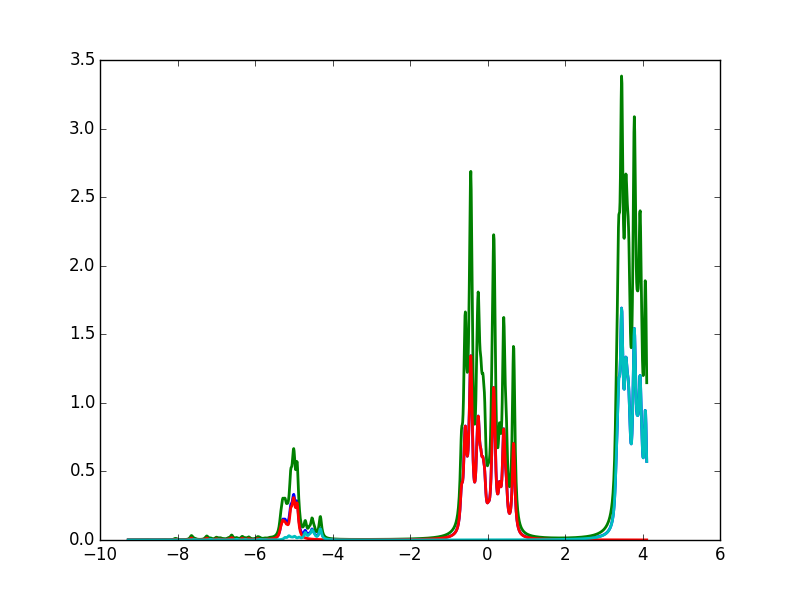
\includegraphics[scale=0.25]{./figs/fig02-01.png}
\caption{The calculated LDOS of a ferromagnetic LSMO model.}
\label{fig01-01}
\end{figure}

Therefore, one can easily plot the calculated LDOS,
\begin{lstlisting}[language=C++]
\$> python [filename].lat.ldos
\end{lstlisting}



\clearpage
\subsection{System default parameters} 
There are several system default parameters like ``isCalculateMu", ``isCalculateBand", etc. to facilitate the TBM$^3$ calculations in the {\bf \#Parameters} block.
Here we list these parameters and their usage.
\begin{center}
\begin{tabular}{  | c | c | c | }
\hline
	\makecell{
	\\
	{\bf Parameter}\\
	\\
	}
	&
	\makecell{
	\\
	{\bf Value}\\
	\\
	}
	&
	\makecell{
	\\
	{\bf Description}\\
	\\
	}\\
\hline
	\makecell{
	\\
		{isCalculateMu}\\
	\\
	}
	&
	\makecell{
		= 1 or 0\\
		(Default value = 0)
	}
	&
	\makecell{
		Enable/disable chemical potential calculation
	}
	\\
\hline
	\makecell{
	\\
		{isCalculateBand}\\
	\\
	}
	&
	\makecell{
		= 1 or 0\\
		(Default value = 0)
	}
	&
	\makecell{
		Enable/disable band structure calculation
	}
	\\
\hline
	\makecell{
	\\
		{isCalculateLDOS}\\
	\\
	}
	&
	\makecell{
		= 1 or 0\\
		(Default value = 0)
	}
	&
	\makecell{
		Enable/disable LDOS calculation
	}
	\\
\hline
	\makecell{
	\\
		{isCalculateVar}\\
	\\
	}
	&
	\makecell{
		= 1 or 0\\
		(Default value = 0)
	}
	&
	\makecell{
		Enable/disable self-consistant loop calculation
	}
	\\
\hline
	\makecell{
	\\
		{need\_MF\_iteration}\\
	\\
	}
	&
	\makecell{
		= 1 or 0\\
		(Default value = 1)
	}
	&
	\makecell{
		Enable/disable mean-field loop iteration.\\ 
		Will be used with ``isCalculateVar".
	}
	\\
\hline
	\makecell{
	\\
		{need\_LLG\_iteration}\\
	\\
	}
	&
	\makecell{
		= 1 or 0\\
		(Default value = 1)
	}
	&
	\makecell{
		Enable/disable LLG loop iteration.\\ 
		Will be used with ``isCalculateVar".
	}
	\\
\hline
	\makecell{
	\\
		{spin}\\
	\\
	}
	&
	\makecell{
		= ``on" or ``off"\\
		(Default value = ``on")\\
	}
	&
	\makecell{
		Construct spin-on/off Hamiltonian
	}
	\\
\hline
	\makecell{
	\\
		{space}\\
	\\
	}
	&
	\makecell{
		= ``normal" or ``nambu" or ``exnambu"\\
		(Default value = ``normal")\\
	}
	&
	\makecell{
		Construct normal/nambu/exnambu Hamiltonian
	}
	\\
\hline
	\makecell{
	\\
		{bondRadius}\\
	\\
	}
	&
	\makecell{
		= real number\\
		(Default value = 1.0)
	}
	&
	\makecell{
		Assign the bond searching radius for each atom.\\
		The value should be larger than\\
		the longest bondVector, $|\delta|(=|$+a+b+c(\#)$|)$.
	}
	\\
\hline
	\makecell{
	\\
		{Mu}\\
	\\
	}
	&
	\makecell{
		= real number\\
		(Default value = 0.0)
	}
	&
	\makecell{
		\;\;Setup the chemical potential by the user.\\
		\;\;If ``isCalculateMu = 1", the value of Mu will be recalculated.\;\;\\
	}
	\\
\hline
	\makecell{
	\\
		{Temperature}\\
	\\
	}
	&
	\makecell{
		= real number\\
		(Default value = 0.00001)
	}
	&
	\makecell{
		Setup the temperature by the user.\\
	}
	\\
\hline
	\makecell{
	\\
		{Nb}\\
	\\
	}
	&
	\makecell{
		= n1,n2,n3\\
	}
	&
	\makecell{
		The number of 3D k-points\\
		 used for several calculation.
	}
	\\
\hline
	\makecell{
	\\
		{ldos\_Nb}\\
	\\
	}
	&
	\makecell{
		= n1,n2,n3\\
		(Default value = Nb)
	}
	&
	\makecell{
		The number of 3D k-points\\
		 used for the LDOS calculation.
	}
	\\
\hline
	\makecell{
	\\
		{ldos\_dE}\\
	\\
	}
	&
	\makecell{
		= real number\\
		(Default value = Nb)
	}
	&
	\makecell{
		The energy step for the LDOS calculation
	}
	\\
\hline
	\makecell{
	\\
		{ldos\_Gamma}\\
	\\
	}
	&
	\makecell{
		= real number\\
	}
	&
	\makecell{
		The broadening factor for LDOS calculation
	}
	\\
\hline
\end{tabular}
\end{center}
\begin{center}
\begin{tabular}{  | c | c | c| }
\hline
	\makecell{
	\\
		{LLG\_dt}\\
	\\
	}
	&
	\makecell{
		= real number\\
		(Default value = 0.01)
	}
	&
	\makecell{
		The rate of the gradient\\
		 for LLG dynamics calculation.
	}
	\\
\hline
	\makecell{
	\\
		{MF\_mix}\\
	\\
	}
	&
	\makecell{
		= real number\\ ( $0\ge$ MF\_mix $\le 1$) \\
		(Default value = 0.1)
	}
	&
	\makecell{
		The mixing parameter for the mean-field\\
		 calculations.
	}
	\\
\hline
	\makecell{
	\\
		{LLG\_diff}\\
	\\
	}
	&
	\makecell{
		= real number\\
		(Default value = 0.001)
	}
	&
	\makecell{
		Convergence criterion for the LLG dynamics.
	}
	\\
\hline
	\makecell{
	\\
		{MF\_diff}\\
	\\
	}
	&
	\makecell{
		= real number\\
		(Default value = 0.001)
	}
	&
	\makecell{
		Convergence criterion for the mean-field calculations.
	}
	\\
\hline
	\makecell{
	\\
		{init\_pair\_magnitude}\\
	\\
	}
	&
	\makecell{
		= real number\\
		(Default value = 1.0)\\
	}
	&
	\makecell{
		\\
		If the pairing orders, $\Delta_{i\alpha\sigma,j\beta\sigma'}$, is not given by the user,\\
		init\_pair\_magnitude will assign a magnitude\\
		for the pairing wave function, $\langle c_{i\alpha\sigma} c_{j\beta\sigma'} \rangle$\\
		to construct the correspond pairing order,\\
		$\Delta_{i\alpha\sigma,j\beta\sigma'} = V_{i\alpha,j\beta}\langle c_{i\alpha\sigma} c_{j\beta\sigma'} \rangle$
		\\\\
	}
	\\
\hline
	\makecell{
	\\
		{init\_pair\_phase}\\
	\\
	}
	&
	\makecell{
		= ``none" or ``random"\\
		(Default value = ``none")\\
	}
	&
	\makecell{
		\\
		If the pairing orders, $\Delta_{i\alpha\sigma,j\beta\sigma'}$, is not given by the user,\\
		and init\_pair\_phase is set to be ``random".\\
		Each pairing wave function, $\langle c_{i\alpha\sigma} c_{j\beta\sigma'} \rangle$\\
		will be assigned with random phase to\\
		construct the correspond pairing order,\\
		$\Delta_{i\alpha\sigma,j\beta\sigma'} = V_{i\alpha,j\beta}\langle c_{i\alpha\sigma} c_{j\beta\sigma'} \rangle$
		\\\\
	}
	\\
\hline
	\makecell{
	\\
		{SOLVER}\\
	\\
	}
	&
	\makecell{
		= ``CPU" or ``GPU"\\
		(Default value = ``GPU")\\
	}
	&
	\makecell{
	\\
		Assign CPU or GPU for the calculation.\\
		If your computer does not have a nvidia-GPU\\
	 	you can choose ``CPU" to perform all of the calculations.
	\\\\
	}
	\\
\hline
\end{tabular}
\end{center}


\clearpage

\subsection{Iterations \& Total Energy}
If we set ``isCalculateVar=1" and some of the {\bf \#Hamiltonian} terms are required for some order parameters from the [filename].lat.ord, it will enable the self-consistant iteration loop and print out the iteration informations in the terminal:
\begin{lstlisting}[language=C++]
Starting...

>> Calculating the chemical potential, Mu.
 Mu         Dest e-den True e-den total_n_diff
 -0.550793   64        -  14        =  50
  2.89742    64        -  48        =  16
  4.62153    64        -  70        = -6
  3.75948    64        -  64        =  0

With spin:on
And space:normal
Total electron count: 64

1  MF-diff>>  0.0391521    1.Q Eng: -207.504   2.Coul Eng: -824.417  Total: -1031.92   Mu: 3.75948
2 LLG-diff>>  0.000306606  1.Q Eng: -207.454   2.Coul Eng: -824.519  Total: -1031.97   Mu: 3.75948
3  MF-diff>>  0.0356134    1.Q Eng: -207.454   2.Coul Eng: -824.519  Total: -1031.97   Mu: 3.76018
4 LLG-diff>>  0.000277408  1.Q Eng: -207.453   2.Coul Eng: -824.612  Total: -1032.06   Mu: 3.76018
5  MF-diff>>  0.0324209    1.Q Eng: -207.453   2.Coul Eng: -824.612  Total: -1032.07   Mu: 3.76081
6 LLG-diff>>  0.000261345  1.Q Eng: -207.456   2.Coul Eng: -824.688  Total: -1032.14   Mu: 3.76081
7  MF-diff>>  0.0295176    1.Q Eng: -207.456   2.Coul Eng: -824.688  Total: -1032.14   Mu: 3.7613
8 LLG-diff>>  0.000246228  1.Q Eng: -207.452   2.Coul Eng: -824.76   Total: -1032.21   Mu: 3.7613
...
...
...
\end{lstlisting}
Above terminal outputs show the self-consistant loop with the choose of ``need\_MF\_iteration=1" and ``need\_LLG\_iteration=1", and both of the mean-field and LLG iterations will be performed one after another.

However, if we set ``need\_MF\_iterations=1" and ``need\_LLG\_iterations=0", all of the quantum part of the Hamiltonian will not be effective, and the termianl will show LLG iterations only: 
\begin{lstlisting}[language=C++]
...
1 LLG-diff>>  0.000306606  1.Q Eng: -207.454   2.Coul Eng: -824.519  Total: -1031.97   Mu: 3.75948
2 LLG-diff>>  0.000277408  1.Q Eng: -207.453   2.Coul Eng: -824.612  Total: -1032.06   Mu: 3.76018
3 LLG-diff>>  0.000261345  1.Q Eng: -207.456   2.Coul Eng: -824.688  Total: -1032.14   Mu: 3.76081
4 LLG-diff>>  0.000246228  1.Q Eng: -207.452   2.Coul Eng: -824.76   Total: -1032.21   Mu: 3.7613
...
\end{lstlisting}

On the other hand, if we set ``need\_MF\_iterations=0" and ``need\_LLG\_iterations=1", all of the classical spin part of the Hamiltonian will not be effective, and the termianl will show mean-field iterations only: 
\begin{lstlisting}[language=C++]
...
1  MF-diff>>  0.0391521    1.Q Eng: -207.504   2.Coul Eng: -824.417  Total: -1031.92   Mu: 3.75948
2  MF-diff>>  0.0356134    1.Q Eng: -207.454   2.Coul Eng: -824.519  Total: -1031.97   Mu: 3.76018
3  MF-diff>>  0.0324209    1.Q Eng: -207.453   2.Coul Eng: -824.612  Total: -1032.07   Mu: 3.76081
4  MF-diff>>  0.0295176    1.Q Eng: -207.456   2.Coul Eng: -824.688  Total: -1032.14   Mu: 3.7613
...
\end{lstlisting}

The above demonstrations is a calculation for the BiFeO$_3$ model as described in {\bf Tutorial E},
\begin{equation}
	H = T + J^H + V^{Coul},
\end{equation}
where $T$ is the hopping, $J^H$ is the Hund's coupling and $V^{Coul}$ is an extra term to describe the long-range Coulomb interactions.


For most of the interactions, there will be a constant term to correct the total energy calculations (except for the Hund's coupling).
The sum of these constant terms are presented during each iteration if the {\bf \#Hamiltonian} block has the correspond term, for example, the ``2.Coul Eng" represents for the constant correction of the Coulomb interactions, $V^{Coul}$.
Here we list all the related constant terms,
\begin{center}
\begin{tabular}{  | c | c | c | }
\hline
	\makecell{
	\\
	{\bf Interaction}\\
	\\
	}
	&
	\makecell{
	\\
	{\bf Shown as}\\
	\\
	}
	&
	\makecell{
	\\
	{\bf Description}\\
	\\
	}\\
\hline
	\makecell{
	\\
		{Quantum energy},\\
	\\
	}
	&
	\makecell{
	\;\;1.Q Eng\;\;\\
	}
	&
	\makecell{
	\;\;Sum over all eigenvalues up to the Fermi surface.\;\;\\
	}
	\\
\hline
	\makecell{
	\\
		\;Screened long-range Coulomb interaction,\;\\
	\\
	}
	&
	\makecell{
	\;\;2.Coul Eng\;\;\\
	}
	&
	\makecell{
    $-\sum_{i=X, |\delta|\le R} \frac{\alpha \;(\langle n_i \rangle - Z_i) ( \langle n_{j} \rangle - Z_{j})}{ |\delta|}\times e^{-|\delta|/R}$\\
	}
	\\
\hline
	\makecell{
	\\
		{On-site Hubbard interaction(intra-orbital)},\\
	\\
	}
	&
	\makecell{
	\;\;3.U Eng\;\;\\
	}
	&
	\makecell{
    $U \sum_{i} (-\langle n_{i\alpha\uparrow} \rangle \langle n_{i\alpha\downarrow} \rangle+\langle c_{i\alpha\uparrow}^\dagger c_{i\alpha\downarrow} \rangle \langle c_{i\alpha\downarrow}^\dagger  c_{i\alpha\uparrow} \rangle)$\\
	}
	\\
\hline
	\makecell{
	\\
		{On-site Dudarev interaction(intra-orbital)},\\
	\\
	}
	&
	\makecell{
	\;\;4.DUJ Eng\;\;\\
	}
	&
	\makecell{
    $(-U/2) \sum_{i} (\langle n_{i\alpha} \rangle^2+\langle \vec s_{i\alpha}\rangle\cdot \langle \vec s_{i\alpha}\rangle)$\\
	}
	\\
\hline
	\makecell{
	\\
		(X)-pairing (on-site and off-site),\\
		X = Singlet, Triplet\\
	\\
	}
	&
	\makecell{
	\;\;5.Pair Eng\;\;\\
	}
	&
	\makecell{
    $\sum_{ij}\sum_{\alpha\beta}\sum_{x} \frac{-1}{V_{ij}} |\Delta_{i\alpha\sigma,j\beta\sigma'}^{(x)}|^2$ \\
	}
	\\
\hline
	\makecell{
	\\
		{Superexchange},\\
	\\
	}
	&
	\makecell{
	\;\;C1.SE Eng\;\;\\
	}
	&
	\makecell{
    $\sum_{ij} J_{ij} \vec S_i\cdot \vec S_j$ \\
	}
	\\
\hline
	\makecell{
	\\
		{DM interaction},\\
	\\
	}
	&
	\makecell{
	\;\;C2.DM Eng\;\;\\
	}
	&
	\makecell{
    $\sum_{ij} \vec D_{ij}\cdot \vec S_i\times \vec S_j$ \\
	}
	\\
\hline
	\makecell{
	\\
		{External magnetic field (classical spin)},\\
	\\
	}
	&
	\makecell{
	\;\;C3.FB Eng\;\;\\
	}
	&
	\makecell{
    $\sum_{i} \vec B_{i}\cdot \vec S_i$ \\
	}
	\\
\hline
\end{tabular}
\end{center}
Note that, the ``quantum energy" is correct only under ``normal" space Hamiltonian but not with ``nambu" or ``exnambu" space due to the particle-hole symmetry is imposed to the situation.
In principal, we should compute the free-energy with finite-temperature calculations instead of total-energy as used for zero-temperatures.
However, since it takes more computations to calculate the free-energy, TBM$^3$ is currently taking the total energy approach, and we might find a better and elegant method to address this issue in the future.

\clearpage


\section{About the Authors}
$\bullet$ {\bf Dr. Yuan-Yen Tai}  joined Los Alamos National Laboratory T-4 group in July 2014.
His research is based on designing of effective models and build efficient algorithms for solving problems in quantum mechanical system, novel emergent material and several nonlinear/statistical systems. 
He designed the first prototype of the TBM$^3$ package in July 2015.
In July 2016, he improved the entire TBM$^3$ framework for a major efficiency gain.
All of the source code (C++ and Python) was written by him.\\
(webpage http://dr-tai.net) \\

$\bullet$ {\bf Dr. Wei Zhu} joined Los Alamos National Laboratory T-4 group in 2016.
His current interests are the topological insulators in strongly correlated systems.
He helped designing the k-space Wannier90 analysis tool for the topological index in TBM$^3$.\\ 

$\bullet$ {\bf Dr. Hongchul Choi} joined Los Alamos National Laboratory T-4 group in 2014.
His current interests are the realization of the topological spin texture in skyrmion compounds with the DFT simulation.
He helped designing the real-space Wannier90 interface, and have been testing the application of TBM3 packages to real compounds.\\
(webpage https://sites.google.com/site/chhchl/home)\\

$\bullet$ {\bf Dr. Jian-Xin Zhu} is the project instructor.
He suggested several useful features to the TBM$^3$ package.\\
(webpage http://www.lanl.gov/expertise/profiles/view/jianxin-zhu)\\



\section{Acknowledgement} 
Y.-Y. T. has special thanks to Dr. Shu-Ting Pi, Dr. Kipton Barros, and Dr. Gia-Wei Chern for many useful discussions and valuable insights for his projects.
H. C. appreciates Dr. Jinwoong Kim for many useful discussions to understand Wannier90 calculation.
This work was supported by U.S. Department of Energy Contract No. DE-AC52-06NA25396 through the LDRD Program, and in part by the Center for Integrated Nanotechnologies, a DOE Basic Energy Sciencesuser facility.

\begin{center}
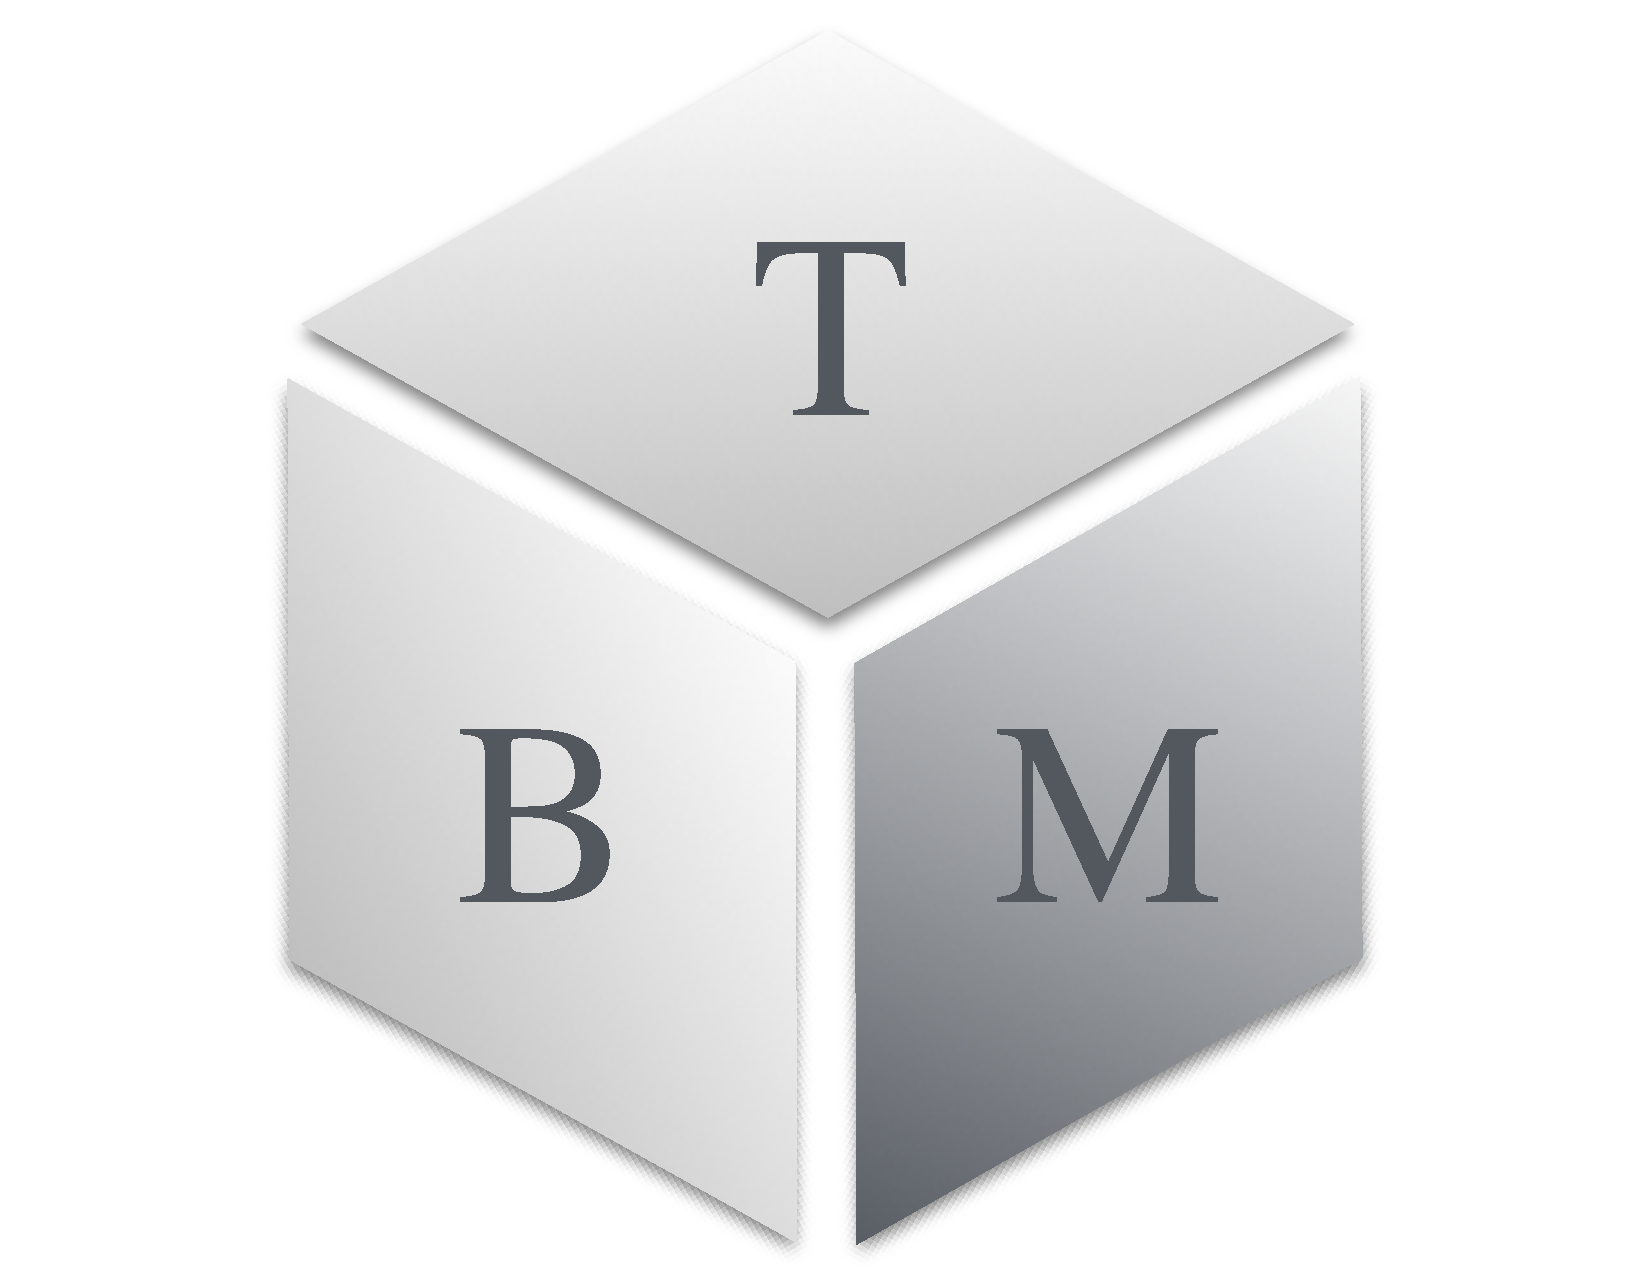
\includegraphics[scale=0.32]{TBMCube-LOGO.pdf}
\end{center}


\begin{center}
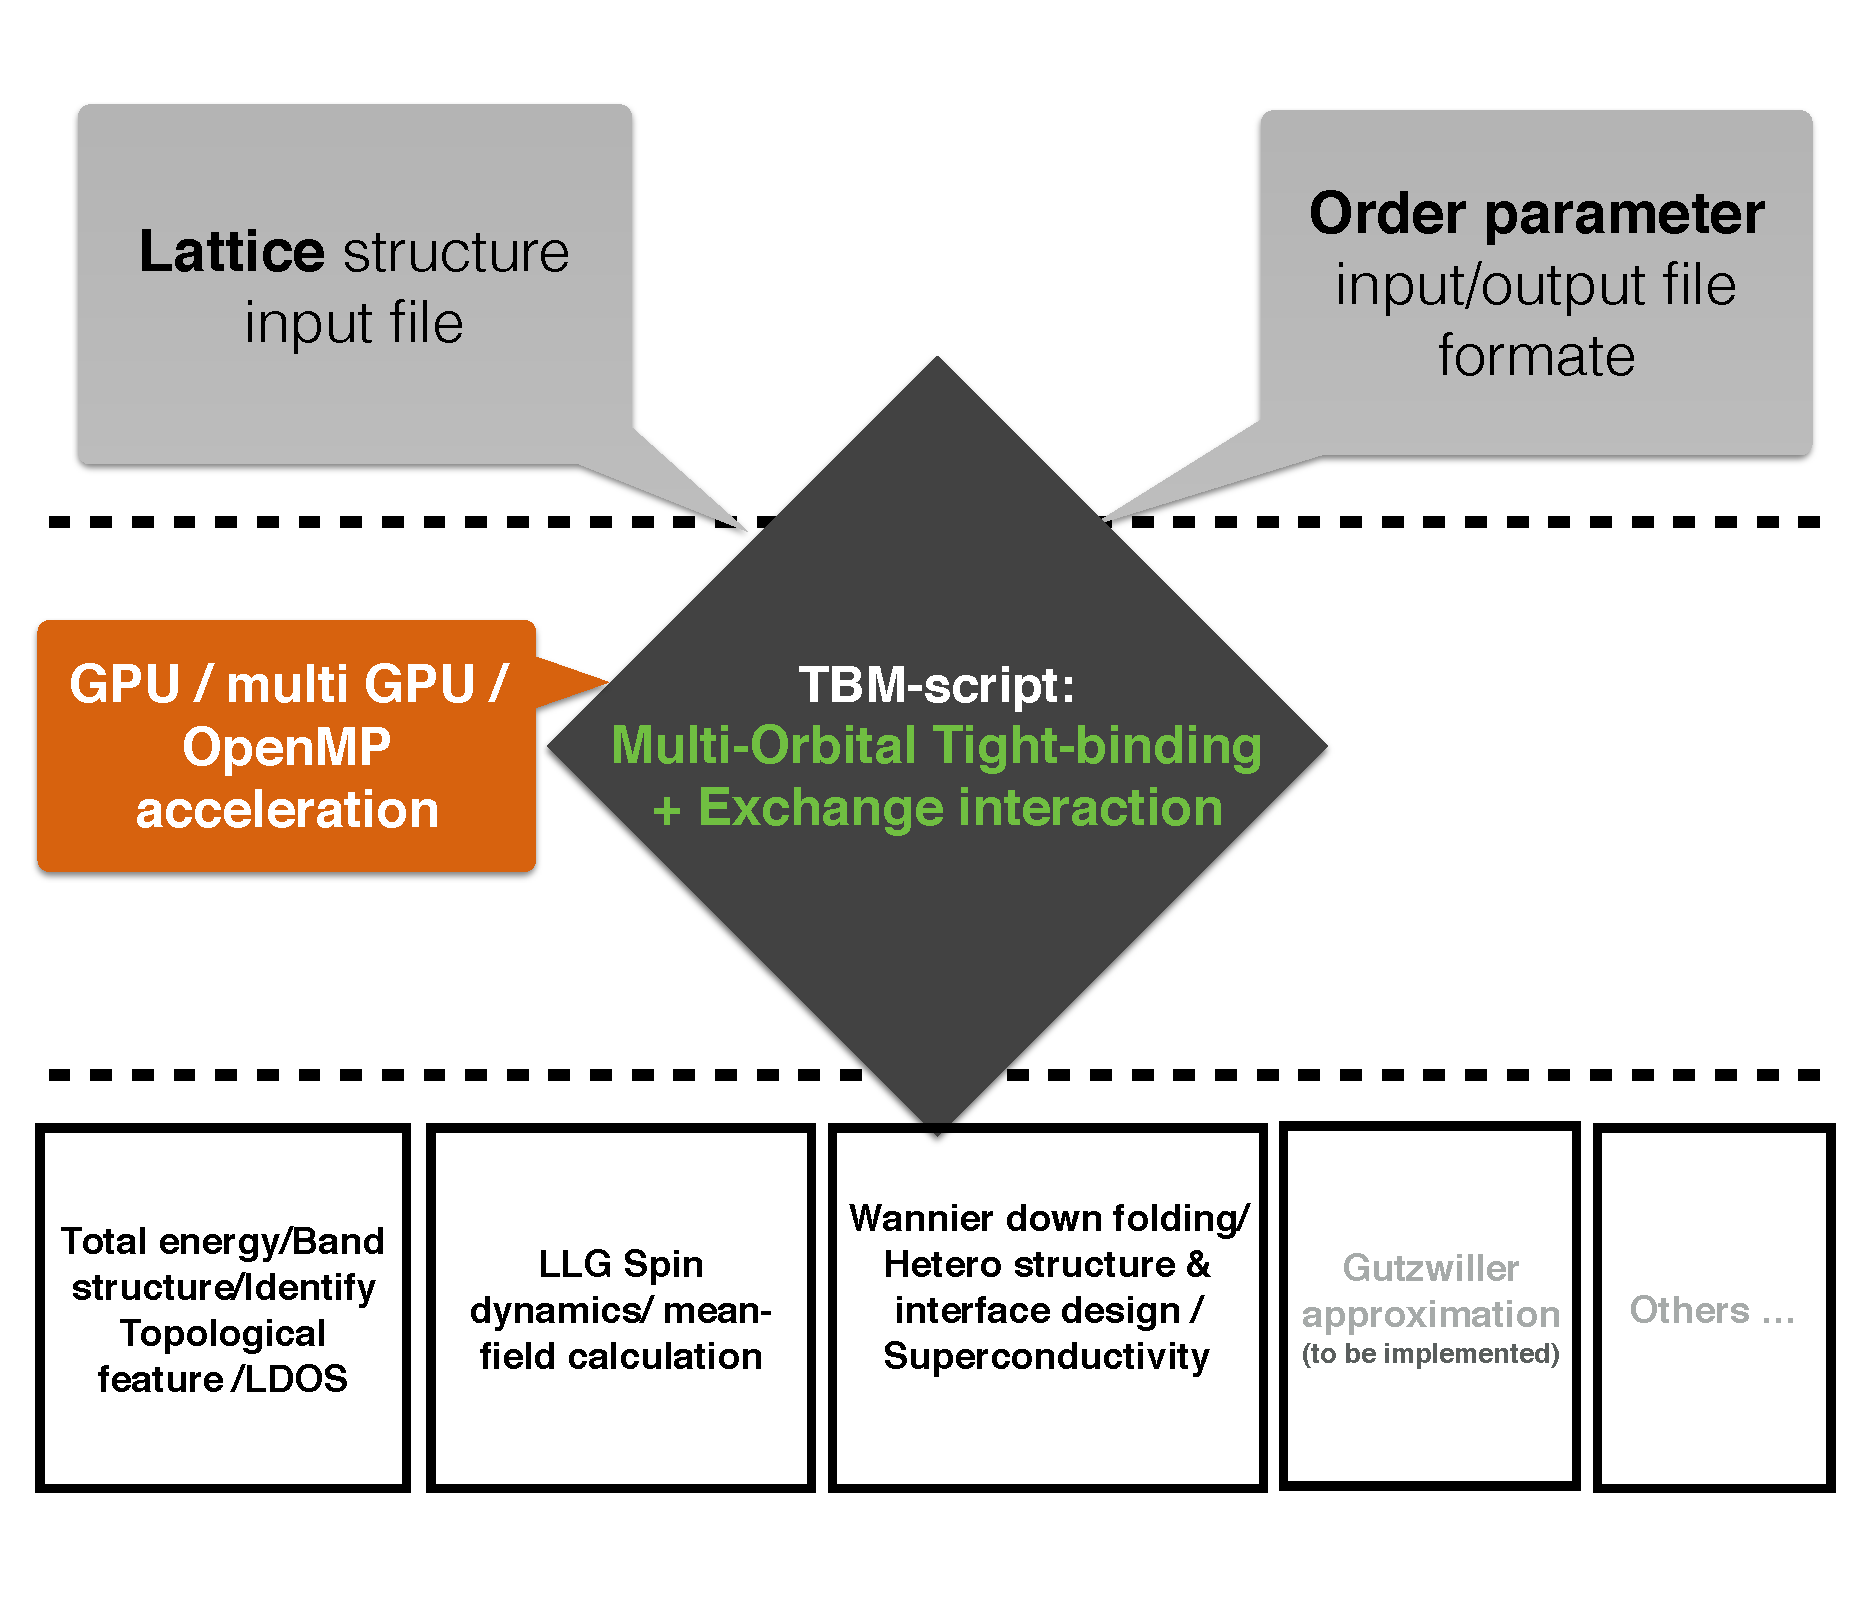
\includegraphics[scale=0.3]{TBMCube.pdf}
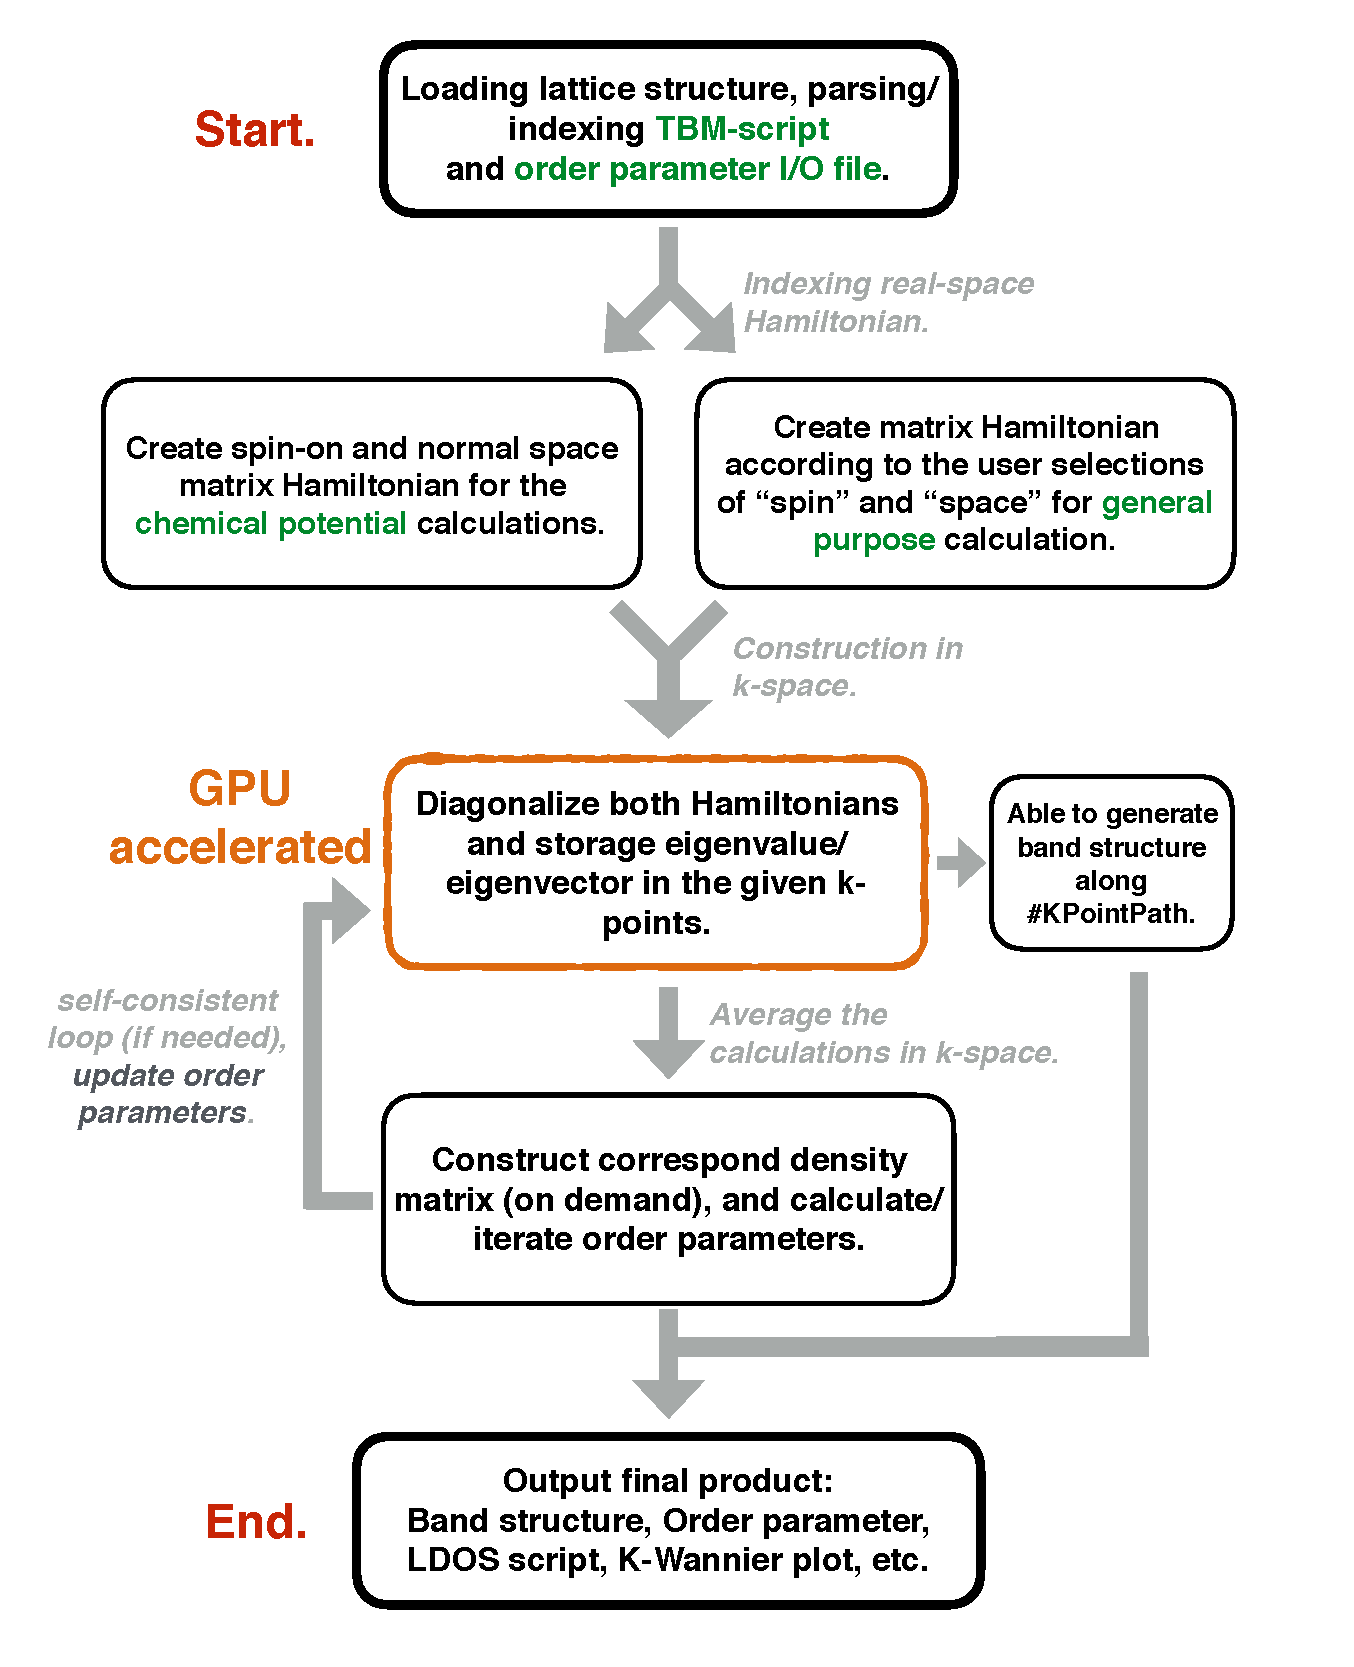
\includegraphics[scale=0.35]{TBMCube-flow.pdf}
\end{center}



\begin{thebibliography}{10}
\bibitem{Philip_book} Philip L. Taylor, \textit{A Quantum Approach to Condensed Matter Physics}, (Cambridge University Press, 2002). 
\bibitem{Cohen2008}Marvin L. Cohen, ``\textit{Essay: Fifty Years of Condensed Matter Physics}", Phys. Rev. Lett. 101 (25) (2008).
\bibitem{Kohn1999}W. Kohn, ``\textit{An essay on condensed matter physics in the twentieth century}", Rev. Mod. Phys. 71 (2): S59. (1999).
\bibitem{Baxter1999}R.J. Baxter, \textit{Exactly solved models in statistical mechanics}, (London, Academic Press, 1982)
\bibitem{BdG}N. N. Bogoliubov, Nuovo Cimento 7, 794 (1958).
\bibitem{BCS} J. Bardeen, L. N. Cooper, J. R. Schrieffer, Physical Review. 106, 162–164. (1957)
\bibitem{Lenz}W. Lenz, Z. Physik 21, 613 (1920)
\bibitem{Ising}E. Ising, Z. Physik 31, 253 (1925)
\bibitem{Bethe}H. Bethe, Z. Physik 71, 205 (1931)
\bibitem{Heisenberg}W. Heisenberg, Z. Physik 49, 619 (1928)
\bibitem{Hubbard}J. Hubbard, Proceedings of the Royal Society of London. 276, 238–257 (1963).
\bibitem{vasp} G. Kresse and J. Hafner, Phys. Rev. B {\bf 47} , 558 (1993); ibid. {\bf 49} , 14 251 (1994).
\bibitem{win} P. Blaha et al., wien2k, Karlheinz Schwarz, Techn. Universit�t Wien, Austria, (2001).
\bibitem{espresso} P. Giannozzi  et al., J.Phys.:Condens.Matter, 21, 395502 (2009)
\bibitem{Jones}
R. O. Jones, \textit{Density functional theory: Its origins, rise to prominence, and future}, Rev. Mod. Phys. 87, 897 (2015)
\bibitem{guziwiller}Claudius Gros ,\textit{Physics of projected wavefunctions}
,Annals of Physics 189, Pages 53-88 (1989) 
\bibitem{dmft1}A. Georges, G. Kotliar, W. Krauth and M. J. Rozenberg, \textit{Dynamical mean-field theory of
strongly correlated fermion systems and the limit of infinite dimensions}, Rev. Mod. Phys.
68, 13 (1996)
\bibitem{dmft2}G. Kotliar, S. Y. Savrasov, K. Haule, V. S. Oudovenko, O. Parcollet and C. A. Marianetti,
\textit{Electronic structure calculations with dynamical mean-field theory}, Rev. Mod. Phys. 78, 865 (2006)
\bibitem{qmc1}L. Pollet, \textit{Recent developments in quantum monte carlo simulations with applications for
cold gases}, Reports on Progress in Physics 75(9), 094501 (2012).
\bibitem{qmc2}W. M. C. Foulkes, L. Mitas, R. J. Needs and G. Rajagopal, \textit{Quantum monte carlo
simulations of solids}, Rev. Mod. Phys. 73, 33 (2001)
\bibitem{cuda} https://developer.nvidia.com/cuda-downloads (the CUDA downlad link).
\bibitem{magma} http://icl.cs.utk.edu/magma/ (the MAGMA download link).
\bibitem{boost} http://www.boost.org (the Boost webpage).
\bibitem{tbm} The code and package of TBM$^3$ is under review, the downloadable link, https://github.com/TDIV/TBM3, will be visible in the near future.
\bibitem{gramat} https://github.com/Anrris/Gramat (the Gramat github repo.).

\bibitem{YYTai01}Yuan-Yen Tai and Jian-Xin Zhu, arXiv:1603.03107 (2016).
\bibitem{HChen01}Hua Chen, Yuan-Yen Tai, C. S. Ting, Matthias J. Graf, Jianhui Dai and Jian-Xin Zhu, Phys. Rev. B {\bf 88}, 184509 (2013).
\bibitem{Haldane88}F. D. Haldane, Phys. Rev. Lett. 61, 2015 (1988).
\bibitem{Thouless82} D. J. Thouless, M. Kohmoto, M. P. Nightingale, and M. den Nijs, Phys. Rev. Lett. {\bf 49}, 405 (1982).
\bibitem{Kane04}C. L. Kane and E. J. Mele, Phys. Rev. Lett. {\bf 95}, 226801 (2004).
\bibitem{Kane05}C. L. Kane and E. J. Mele, Phys. Rev. Lett. {\bf 95}, 146802 (2005).
\bibitem{XLQi2011} X. L. Qi, Phys. Rev. Lett. {\bf 107}, 126803 (2011).
\bibitem{XDai2011} R. Yu, X. L. Qi, A. Bernevig, Z. Fang, and X. Dai, Phys. Rev. B 84, 075119 (2011).
\bibitem{Vanderbilt2011}A. A. Soluyanov and D. Vanderbilt, Phys. Rev. B 83, 035108 (2011).
\bibitem{W90-1}N. Marzari and D. Vanderbilt, Phys. Rev. B 56, 12847 (1997)
\bibitem{W90-2}I. Souza, N. Marzari and D. Vanderbilt, Phys. Rev. B 65, 035109 (2002)
\bibitem{W2W}J.Kunes, R.Arita, P.Wissgott, A.Toschi, H.Ikeda, K.Held, Comp.Phys.Commun. 181, 1888 (2010) 

\bibitem{JXZhuBook} Jian-Xin Zhu, \textit{Bogoliubov-de Gennes Method and Its Applications}, (Springer International Publishing Switzerland, 2016).




\end{thebibliography}

\end{document}



